\chapter[Analysis]{\r Analysis (rethink title)}\label{chap:analysis}

This chapter constitutes the core of this dissertation. It explains the conducted analysis, beginning with a general overview, followed by an explanation of the samples, triggers, and object definitions. An entire section discusses the meson reconstruction techniques used, which are crucial to the analysis. Subsequently, it covers the criteria applied in event selection and describes how the signal and background have been modelled. Finally, it presents the expected upper limits of the branching ratio for each decay channel. These are $\text{H}\decaysto \phi\gamma$ with further $\phi\decaysto \pi^+\pi^-\pi^0$, $\text{H}\decaysto \omega\gamma$ with further $\omega\decaysto \pi^+\pi^-\pi^0$, $\text{H}\decaysto \text{D}^{*0}\gamma$ with further $\text{D}^{*0}\decaysto \text{D}^{0}\pi^{0}/\gamma$, $\text{D}^{0}\decaysto K^{-}\pi^{+}$ and $\text{H}\decaysto \text{D}^{*0}\gamma$ with further $\text{D}^{*0}\decaysto \text{D}^{0}\pi^{0}/\gamma$, $\text{D}^{0}\decaysto K^{-}\pi^{+}\pi^{0}$.

This analysis represents an initial approach to compute these upper limits, and there are many more steps required to cross-check the methodology before attempting an actual measurement. Therefore, only an estimation using simulated data is computed. The chapter concludes by addressing the steps needed before data unblinding and obtaining the final experimental measurement, as well as suggesting ideas for optimizing and improving the results.

\section{Analysis overview}\label{sec:analysis_overview}

This analysis uses data from proton-proton collisions corresponding to an integrated luminosity of 39.54 fb$^{-1}$ at $\sqrt{s}=$13 TeV, collected by the CMS detector at the LHC in 2018 during Run 2. It does not target any specific production mode of the Higgs boson, but instead considers all production modes, which will be dominated mainly by gluon fusion (ggH) with a minor contribution from vector boson fusion (VBF). Nevertheless, it can be interesting to target specific production modes, as this can reduce background contamination by individually studying and applying dedicated techniques to each mode, and could be part of further extensions of this analysis. The decays under study are of the form H$\decaysto M\gamma$, the mesons $M$ are a $\phi$, $\omega$ and $\text{D}^{*0}$, each further decaying into two charged particles and a third (and fourth) neutral one, as shown in Table \ref{tab:Higgs_rare_decays_three}.
\begin{table}[ht]
    \centering
    \begin{tabular}{ll}
        $\text{H}\decaysto \phi\gamma$ ,& $\phi\decaysto \pi^+\pi^-\pi^0$ \\
        $\text{H}\decaysto \omega\gamma$ ,& $\omega\decaysto \pi^+\pi^-\pi^0$\\
        $\text{H}\decaysto \text{D}^{*0}\gamma$ ,& $\text{D}^{*0}\decaysto \text{D}^{0}\pi^{0}/\gamma,\ \text{D}^{0}\decaysto \text{K}^{-}\pi^{+}$\\
        $\text{H}\decaysto \text{D}^{*0}\gamma$ ,& $\text{D}^{*0}\decaysto \text{D}^{0}\pi^{0}/\gamma,\ \text{D}^{0}\decaysto \text{K}^{-}\pi^{+}\pi^{0}$
    \end{tabular}
    \caption{Higgs rare decays studied in this analysis.}
    \label{tab:Higgs_rare_decays_three}
\end{table}

Therefore, the final states of interest consist of an isolated and energetic photon, a charged meson pair, and photons compatible with a third (and sometimes fourth) neutral particle, with no additional leptons (e$/\mu$). 

The branching fractions of rare Higgs boson decays to a meson and photon can be computed using a factorization approach in QCD. The calculation considers both direct and indirect contributions, as explained in the first chapter and depicted in Figure \ref{fig:Higgs_rare_decay_veritces}. The interference between these components is significant, and in the SM, the indirect component dominates. Then, the Higgs boson couplings to light quarks are probed by searching for modifications in this branching fraction due to interference effects.

As previously explained, given the exotic nature of the decays under study, the theoretical decay widths being so small, and the large hadronic background at the LHC, we cannot aim for precise measurements of the branching fractions. Instead, the end goal of this thesis is to calculate expected upper limits on the branching ratios of the aforementioned Higgs boson decays, using Monte Carlo (MC) samples to model the SM expected signal. To obtain an actual measurement, this initial estimation requires further refinement and improvement, such as considering additional background sources or systematic uncertainties. A more extensive list is provided at the end of this chapter.

It is worth noting that this analysis and the one studying the three decays involving a $\rho^0$, $\phi$ and K$^{*0}$ meson in the upper half of Table \ref{tab:Higgs_rare_decays} are remarkably similar, and only differ by the consideration of neutral particles, which are more challenging to reconstruct than charged ones. The framework used for this analysis builds upon the existing framework for these simpler two-body decays currently under analysis by the CMS collaboration. To extend their study to include three-body decays involving neutral particles, our main focus has been on accurately recovering the missing neutral particles.

\section{Samples and triggers}\label{sec:samples_triggers}

To develop this analysis, the data file format used is one designed by CMS, which is an extended version of \verb+NANOAOD+. It is based on the official \verb+NANOAODv9+ recipe and includes the reconstructed mesons, as described in Section \ref{sec:objects}, as additional objects. The \verb+NANOAOD+ format consists of an Ntuple-like structure used by CMS, which can be read using bare \verb+ROOT+ \cite{CERN:root}, and containing the per-event information that is needed in most generic analyses \cite{CMS:NanoAOD}. This analysis is performed using the \verb+ROOT+ data analysis framework, an open-source data analysis tool commonly used in high energy physics written mainly in C++.

\subsection{Data and triggers}\label{subsec:data_tau_trigger}

Events are selected from proton-proton collision data at a center-of-mass energy of $\sqrt{s}=$13 TeV and a bunch spacing of 25 ns, collected by the CMS experiment during the LHC's Run 2 in 2018, corresponding to a total integrated luminosity of 39.54 fb$^{-1}$. Good run ranges and luminosity blocks are chosen based on criteria encoded in a golden JSON file.

To filter the events, a high-level trigger, named \verb+HLT_Photon35_TwoProngs35+, is employed. This trigger selects a photon with $\pT^{\gamma} > 35\ \GeV$ and a ditrack system with $\pT^{\text{jet}} > 35\ \GeV$, after passing through the L1 trigger, which also imposes rapidity restrictions of $\abs{\eta^{\gamma}}<2.1$ and $\abs{\eta^{\text{jet}}}<2.1$. The trigger is applied to both data and MC. Introduced in 2018, this trigger recorded events enriched in gluon fusion production of the Higgs boson and VBF that were not registered by the dedicated trigger, providing an effective luminosity of 39.54 fb$^{-1}$. The datasets used in gluon fusion analysis, along with their integrated luminosities, are detailed in Table \ref{tab:ggH_datasets}.

\begin{table}[ht]
    \centering
    \begin{tabular}{|c|c|c|}
        \hline
        \multicolumn{1}{|c|}{\cellcolor{lightgray}Year} & \cellcolor{lightgray}Dataset & \cellcolor{lightgray}Integrated luminosity [fb$^{-1}$] \\ \hline
        2018    & \verb+/Tau/Run2018B-UL2018+  & 0.67 \\
        2018    & \verb+/Tau/Run2018C-UL2018+  & 6.94 \\
        2018    & \verb+/Tau/Run2018D-UL2018+  & 31.93 \\ \hline
    \end{tabular}
    \caption{Datasets used in the gluon fusion analysis from the campaign MiniAODv2 of the MINIAOD data tier.}
    \label{tab:ggH_datasets}
\end{table}

\subsection{Background simulation}

The background estimation will ultimately rely solely on data. However, in the early stage of this analysis, simulated samples are used to understand the background processes affecting the different selected final states. The main background process for the gluon fusion production mode is a single photon and jets, denoted as $\gamma$ + jets throughout the analysis.

Every background event is generated at leading order (LO) precision using the MADGRAPH5 generator \verb+MG5_aMC@NLO+ \cite{Alwall:2014hca} and POWHEG \cite{Alioli:2010xd}, while PYTHIA8 \cite{Sjostrand:2014zea} is used for the hadronization. For all simulations, the NNPDF 3.1 \cite{NNPDF:2017mvq} next-to-next-to-leading-order (NNLO) parton distribution functions (PDFs) are used, while the modelling of the underlying event is generated using the CMS Pythia 5 (CP5) tunes \cite{CMS:2019csb}. The Run 2 legacy reconstruction algorithms \cite{Elmetenawee:2020emw} are used for all the MC and data samples. The campaign and global tag used to produce the background and signal MC samples are \verb+RunIISummer20UL18MiniAODv2-106X+ and \verb+upgrade2018_realistic_v16_L1v1+, respectively. Table \ref{tab:MC_samples} summarizes the list of datasets used for the study along with their cross sections \cite{CERN:xsdb}.

\begin{table}[ht]
    \centering
    \begin{tabular}{|l|c|}
        \hline
        \multicolumn{1}{|c|}{\cellcolor{lightgray}Monte Carlo name} & \cellcolor{lightgray}Cross section [pb] \\ \hline
        \verb+GJets_HT-40To100_TuneCP5_13TeV-madgraphMLM-pythia8+  & 18540 (LO) $\times$ 1.26 \\
        \verb+GJets_HT-100To200_TuneCP5_13TeV-madgraphMLM-pythia8+  & 8644 (LO) $\times$ 1.26 \\
        \verb+GJets_HT-200To400_TuneCP5_13TeV-madgraphMLM-pythia8+  & 2183 (LO) $\times$ 1.26 \\
        \verb+GJets_HT-400To600_TuneCP5_13TeV-madgraphMLM-pythia8+  & 260.2 (LO) $\times$ 1.26 \\
        \verb+GJets_HT-600ToInf_TuneCP5_13TeV-madgraphMLM-pythia8+  & 86.58 (LO) $\times$ 1.26 \\ \hline
    \end{tabular}
    \caption{MC samples used to generate the $\gamma$ + jets background. The normalization of $\gamma$ + jets is scaled by 1.26 to account for higher-order contributions \cite{CMS:2018qao}.}
    \label{tab:MC_samples}
\end{table}

\subsection{Signal simulation}

The Higgs boson production modes used, ggH and VBF, are generated at next-to-leading order (NLO) using the POWHEGv2 event generator extended with the MiNLO procedure \cite{Hamilton:2012np}. The production rates and kinematic distributions for the Higgs boson with $m_\text{H}=125\ \GeV$ are assumed throughout. In particular, the cross section for ggH and VBF are computed at NNLO in QCD and NLO in electroweak accuracy, resulting in 48.58 pb and 3.78 pb, respectively, as provided by the LHC Higgs Cross Section Working Group in Ref. \cite{LHCHiggsCrossSectionWorkingGroup:2016ypw}.

The decay of the Higgs boson is handled by Pythia, and it does not simulate direct and indirect effective vertices. The expected SM branching fractions of the Higgs rare decays are previously shown in Table \ref{tab:Higgs_rare_decays_values}.%: $\mathcal{B}(\text{H}\decaysto \phi\gamma) = (2.31 \pm 0.11)\times 10^{-6}$ and $\mathcal{B}(\text{H}\decaysto \omega\gamma) = (1.48 \pm 0.08)\times 10^{-6}$, while $\mathcal{B}(\text{H}\decaysto \text{D}^{*0}\gamma)$ has not yet been computed.
In the analysis, however, the branching ratios are set to
\begin{equation*}
    \mathcal{B}(\text{H}\decaysto \phi\gamma) = \mathcal{B}(\text{H}\decaysto \omega\gamma) = \mathcal{B}(\text{H}\decaysto \text{D}^{*0}\gamma) = 1\ .
\end{equation*}
This is because when computing the upper limit, the obtained value is directly the measured upper limit of the branching ratio itself. If we were to set the branching fractions to the SM values, the measured quantities would be the signal strengths, i.e., the factors by which the observed fractions exceed the SM values. The branching fractions of the meson decays used are also shown in Table \ref{tab:Higgs_rare_decays}, but further detailed in Table \ref{tab:Meson_decay_br}.

\begin{table}[!ht]
    \centering
    \begin{tabular}{|l@{}l|c|}
        \hline
        \multicolumn{2}{|c|}{\cellcolor{lightgray}Meson decay channel} & \multicolumn{1}{c|}{\cellcolor{lightgray} SM $\mathcal{B}$ (\%)} \\ \hline
        $\phi$&$\decaysto \pi^+\pi^-\pi^0$     & $15.4 \pm 0.4$   \\
        $\omega$&$\decaysto \pi^+\pi^-\pi^0$   & $89.2 \pm 0.7$   \\
        $\text{D}^{*0}$&$\decaysto \text{D}^{0}\pi^0$        & $64.7 \pm 0.9$   \\
        $\text{D}^{*0}$&$\decaysto \text{D}^{0}\gamma$       & $35.3 \pm 0.9$   \\
        $\text{D}^{0}$&$\decaysto \text{K}^{-}\pi^{+}$           & $3.947 \pm 0.030$   \\
        $\text{D}^{0}$&$\decaysto \text{K}^{-}\pi^{+}\pi^0$      & $14.4 \pm 0.5$   \\
        \hline
    \end{tabular}
    \caption{Meson decay branching ratios used throughout the analysis, from the PDG \cite{PDG}.}
    \label{tab:Meson_decay_br}
\end{table}

\section{Object definitions}\label{sec:objects}

This analysis primarily relies on photons and charged tracks to extract the final state signature of exclusive hadronic decays, while also making use of other physics objects such as additional leptons (or the lack thereof). All used objects, except the mesons, are discussed in this section, with the next section dedicated solely to meson reconstruction.

\subsection{Primary vertex}
To consider an event, it must contain at least one primary vertex (PV), which is regarded as the vertex of the hard interaction. There should be a minimum of four tracks associated with the selected primary vertex (from the Higgs boson, the photon and the ditrack system). For events with multiple selected vertices, the PV is chosen to be the vertex corresponding to the hardest scattering in the event, determined using tracking information alone, as described in Ref. \cite{Contardo:2015bmq}.

%\subsection{Jets}
%During the reconstruction of a proton-proton (pp) collision, jets are often reconstructed with a $\pT$ that differs from that of the final-state particles within the jet. The jet energy corrections (JEC) adjust the reconstructed jet energy to match the true energy of the final-state particles. The CMS collaboration has developed a factorized approach to these JEC, consisting of multiple levels that correct various physics or detector effects. This approach provides flexibility in the corrections to suit various types of analyses. These correction levels are commonly referred to as L1FastJet, L2Relative, L3Absolute, and L2L3Residual.

%Jets are reconstructed from particle flow (PF) candidates using the anti-$k_\text{T}$ clustering algorithm with a distance parameter of $R = 0.4$ as implemented by FastJet \cite{Cacciari:2011ma}. Jets within this small cone (referred to as AK4 jets for $R = 0.4$) are selected among those with $\pT > 20\ \GeV$ and $\abs{\eta} < 4.7$ for forward tagging. At the LHC, a significant number of pp collisions occur simultaniously during one bunch crossing, with soft ones contaminating the collision of interest. To mitigate this effect, known as \textit{pileup} (PU), charged hadrons not originating from the primary vertex are removed using the charged hadron subtraction (CHS) algorithm \cite{CMS:2014ata, Perloff:2012wpa}. The tight pileup ID criterion is applied to reduce the contamination of jets with $\pT < 50\ \GeV$ initiated by the pileup interactions. Jets are corrected for the response inside the detector, differentially in $\abs{\eta} - \abs{\phi}$, for the pileup contributions, and for data only, the residual difference observed between data and simulation.

%In the current analysis version, the \verb+Summer19UL+ jet energy corrections set is used-%, as well as the DeepJet tagging algorithm with the medium working point to identify b-jets \cite{Bols:2020bkb}.

\subsection{Photons}\label{subsec:photons}
Photon candidates are reconstructed as SuperCluster objects in the ECAL with $\ET > 38\ \GeV$ and $\abs{\eta^{\gamma}} < 2.1$ in both the barrel and endcap regions. In addition, photons have to satisfy the multivariate analysis (MVA) based selection identification (mvaID) criteria following the \verb+Fall17IsoV2+ recipe \cite{CMS:2020uim}. For the production mode used, the mvaID provides 80\% (90\%) signal selection efficiency for the endcap (barrel) region. The mvaID criteria include photon isolation, charged hadron isolation, and require photons to pass shower shape preselection cuts \cite{Rembser:2019ijh}. The photon's ECAL cluster must be inconsistent with charged particle tracks reconstructed in the silicon tracker to reject electrons faking photons, achieved using a conversion safe electron veto. Residual $\ET$ -dependent photon energy scale and smearing corrections are applied. Additional photons with looser requirements ($\ET > 20\ \GeV$ and the WP90 version of the photonID) are also vetoed to reduce the potential contribution of diphotons. Table \ref{tab:photon_selection} summarizes the criteria for photon selection.

\begin{table}[!ht]
    \centering
    \begin{tabular}{|l|c|}
        \hline
            \multicolumn{2}{|c|}{\cellcolor{lightgray}Selection criteria ($\gamma$ from PV)}\\ \hline
            $\pT^{\gamma}$            &$>38$ GeV\\
            $\abs{\eta^{\gamma}}$       &$<2.1$ \\
            mvaID                       &WP90/WP80 \\
            electron Veto               &Yes \\\hline
        \end{tabular}
    \caption{Selection criteria applied to the photon from the primary vertex.}
    \label{tab:photon_selection}
\end{table}

An additional correction was attempted, involving shifting the photon's origin to that of the PV of the meson. This slight adjustment to the initial coordinates led to a minor change in the four-momentum variables of the photon, but it did not consistently reduce the discrepancy with the generation-level particle values. Consequently, it was discarded and not used.

\section{Meson reconstruction}\label{sec:meson_reconstruction}

The $\phi$, $\omega$ and $\text{D}^{*0}$ mesons decay products are reconstructed using charged particle tracks measured in the tracker, as well as energy deposited in the ECAL compatible with neutral particles coming also from the PV. For the $\phi$ and $\omega$ mesons, the targeted charged ditrack is $\pi^\pm\pi^\mp$, while for the $\text{D}^{*0}$ meson the charged ditrack is $\text{K}^{-}\pi^{+}$.

In the following sections, the term \textit{ditrack system} will refer to the system of the two charged tracks. Even though they not form a real particle, notions like ditrack mass will be used (understood as the mass component of the sum of the four-momenta of both tracks). To refer to the meson originating from the PV, namely $\phi$, $\omega$ and $\text{D}^{*0}$, terms like \textit{meson} or \textit{full meson} will be used, emphasizing that the neutral particles have been accounted for. Some considerations have been made to precisely reconstruct the full meson, as described in the following subsections.

\subsection{Track selection}
To be selected, the tracks need to satisfy a ``high purity'' reconstruction criteria, which considers the number of tracker layers with hits, track fit quality, and the impact parameter values relative to their uncertainties. For a detailed description of the algorithm, refer to Ref. \cite{CMS:2014pgm}.

\subsection{Meson decay vertex}
The meson decay vertex is determined using the standard CMSSW \cite{CMSSW} kinematic vertex fitting package, as described in Ref. \cite{Prokofiev:2005zz}. Using the candidate's decay vertex and its associated momentum, a newly fitted transient track is constructed to represent the meson candidate. Then, for each primary vertex, the track is extrapolated to the nearest point in 3D space. The meson vertex's longitudinal distance is required to be within 24 cm from the centre of the detector.

\subsection{Isolation}
To ensure good track selection, a dedicated isolation criterion of the candidate based on the tracks is used. This dimensionless isolation parameter (Iso) is determined from the meson's momentum and other tracks within a cone of radius $\Delta R = 0.3$ around the ditrack system's direction. Only tracks with $\pT > 0.9\ \GeV$ associated with the same meson vertex are considered, excluding the charged-hadron candidates that define the ditrack. The definition is as follows:
\begin{equation*}
    \text{Iso} = \frac{\pT^{\text{meson}}}{\pT^{\text{meson}}+\sum_{\text{trk}}{\abs{\pT^{\text{trk}}}}}
\end{equation*}
A high isolation value will be required to consider a meson candidate (over 0.9).

\subsection{Photons from the neutral particle decays}\label{subsec:photons_neutral}
For each selected ditrack, up to two photons with $\pT > 5 \ \GeV$ are recovered in a small cone of $\Delta R = 0.05$ ($\Delta R = 0.10$ for $\text{D}^{*0}$ three-body channel) around the ditrack direction. These photons account for the recovery of neutral particles, as $\pi^{0}\decaysto\gamma\gamma$ in $\sim 98.8\%$ with $c\tau=25$ nm \cite{PDG}, so their origin can be considered the same as that of the meson decay. Generation-level MC reveals that photons coming from neutral particle decays that in turn come from the three-body decays are very collimated with the ditrack system. In the case of the $\phi$/$\omega$ channels and the $\text{D}^{*0}$ channel when $\text{D}^{0}$ decays into three bodies, these photons directly originate from the $\pi^0$ of the three-body decay. In the case of the $\text{D}^{*0}$ channel, additional photons come either directly from $\text{D}^{*0}\decaysto \text{D}^{0}\gamma$ or from the decay of the $\pi^0$ from $\text{D}^{*0}\decaysto \text{D}^{0}\pi^0$. Unlike the photons described in Section \ref{subsec:photons}, these photons are not corrected for discrepancies between data and MC. This adjustment is necessary for precise measurements.

\subsection{Ditrack mass hypothesis}
The invariant mass of the refitted ditrack system is also used to reduce contamination from background events. The mass of the pair, assuming the charged-pion hypothesis for the two tracks, is coherent with the charged components of the $\phi$ and $\omega$ mesons. Since the ditrack system is not a real resonance, its mass is very wide but consistent and useful for reducing background events. In the case of the $\text{D}^{*0}$ channel, two scenarios are considered. On the one hand, when $\text{D}^{0}$ decays into a pair of charged particles (kaon-pion) the ditrack system's invariant mass is a real narrow resonance (i.e., $\text{D}^{0}$) consistent with the mass of that meson. On the other hand, when $\text{D}^{0}$ decays into a pair of charged particles and a neutral pion, one finds the same scenario as for the $\phi$/$\omega$ decay channels.

The exact used selection criteria will be presented at the end of this section, but it is worth noting that for the $\phi$/$\omega$ three-body decays involving a $\pi^0$, the mass of the ditrack is approximately two-thirds of the full meson's mass (each pion carries roughly a third of the energy).

Furthermore, instead of recovering the ditrack invariant mass by only retrieving the mass component of the sum of both four-momenta, the CMSSW \cite{CMSSW} kinematic fit has been employed. To study the performance of this fit, it is useful to define the \textit{residual} as the difference between the reconstructed values and the corresponding generation-level ones. Figure \ref{fig:kinematic_fit_residuals} displays the residual of the ditrack invariant mass reconstruction with (red) and without (blue) the kinematic fits with vertex constraint for the decay modes involving $ \phi$ or D$^{*0}$ mesons.
\begin{figure}[!ht]
    \captionsetup[subfigure]{labelformat=empty}
    \vspace*{-0.2cm}
    \centering
    \setlength{\mylength}{\textwidth}
    \begin{subfigure}[t]{0.50\mylength}
            \centering
            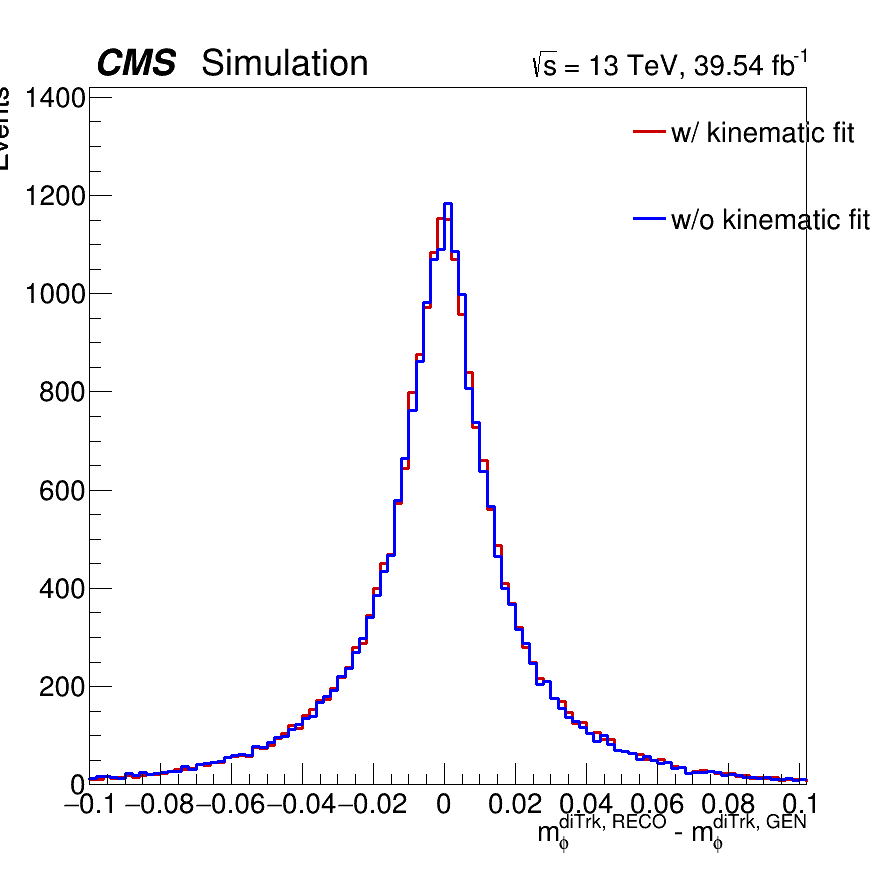
\includegraphics[width=0.49\mylength]{resources/plots/Phi3_kinematic_fit_residual.png}
            \vspace*{-0.2cm}
            \caption{\footnotesize (a)}
    \end{subfigure}%
    %\begin{subfigure}[t]{0.50\mylength}
    %        \centering
    %        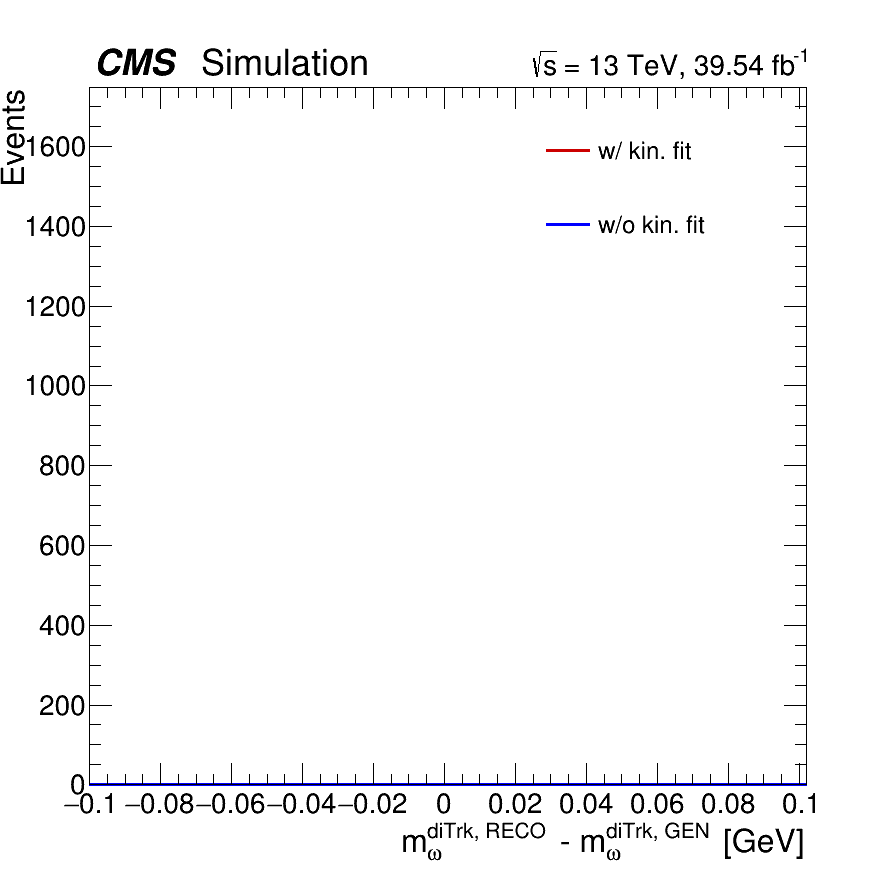
\includegraphics[width=0.49\mylength]{resources/plots/Omega_kinematic_fit_residual.png}
    %\vspace*{-0.2cm}
    %        \caption{\footnotesize (b)}
    %\end{subfigure}%\begin{subfigure}[t]{0.50\mylength}\baselineskip
    \vskip\baselineskip
    \vspace*{-0.5cm}
    \begin{subfigure}[t]{0.50\mylength}
            \centering
            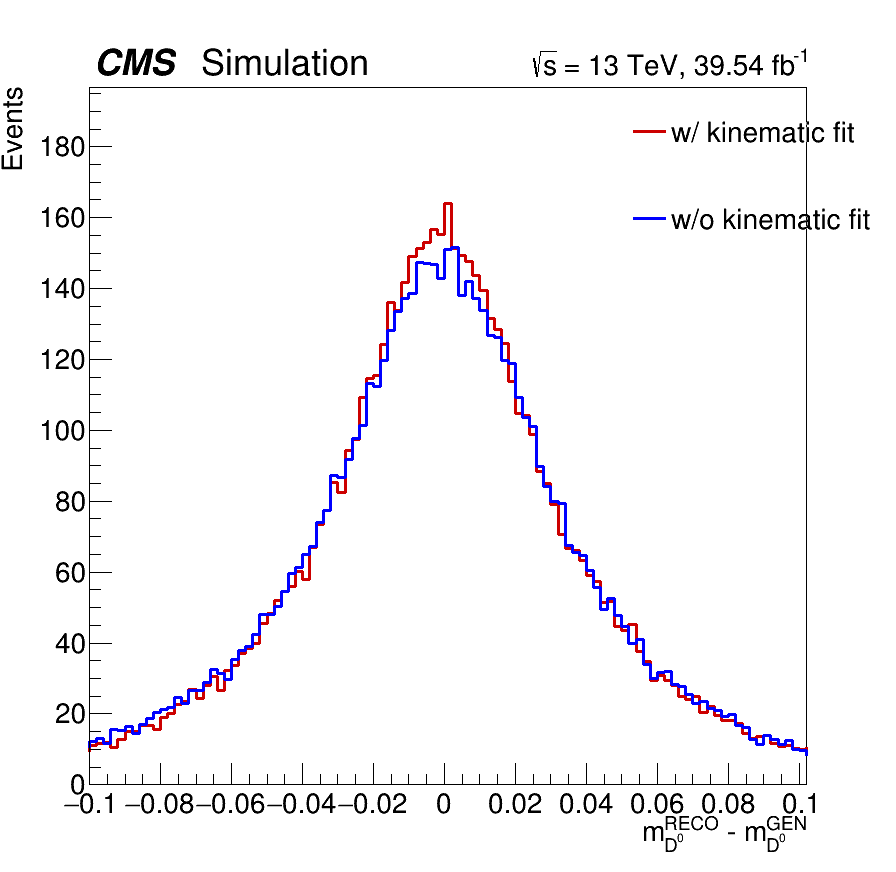
\includegraphics[width=0.49\mylength]{resources/plots/D0Star_2body_kinematic_fit_residual.png}
            \vspace*{-0.2cm}
            \caption{\footnotesize (b)}
    \end{subfigure}%\begin{subfigure}[t]{0.50\mylength}
    \begin{subfigure}[t]{0.50\mylength}
            \centering
            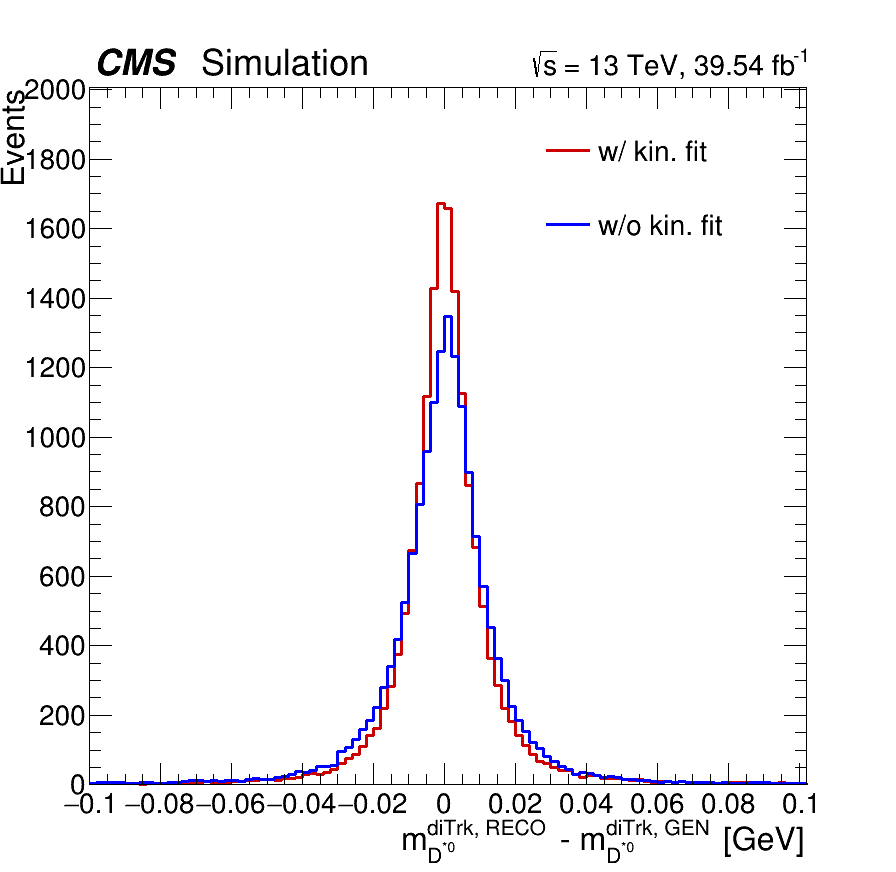
\includegraphics[width=0.49\mylength]{resources/plots/D0Star_3body_kinematic_fit_residual.png}
            \vspace*{-0.2cm}
            \caption{\footnotesize (c)}
    \end{subfigure}%
    \vspace*{-0.0cm}
    \caption{Ditrack mass residuals with (red) and without (blue) kinematic fits for the different decay channels. (a) is for $\phi$, (b) is for $\text{D}^{*0}$ 2-body, and (c) is for $\text{D}^{*0}$ 3-body.}
    \label{fig:kinematic_fit_residuals}
    \vspace*{-0.0cm}
\end{figure}
Table \ref{tab:kinematic_fit_RMSE} shows the root mean squared errors (RMSE) with respect to generation-level, both with and without the kinematic fit, for each channel involving $ \phi$ or D$^{*0}$ mesons. Applying the kinematic fit improves the reconstructed ditrack invariant mass values for all channels. The $\omega$ decay channel behaves identically to the $\phi$ channel.
\begin{table}[!ht]
    \centering
    \begin{tabular}{|l|c|C{2.9cm}@{}c|}
        \hline
        \cellcolor{lightgray}Decay channel & \cellcolor{lightgray}RMSE without kinematic fit & \multicolumn{2}{c|}{\cellcolor{lightgray}RMSE with kinematic fit} \\ \hline
        $\phi$          &36.7 MeV   &33.4 MeV  & (-9\%)   \\
        %\r$\omega$        &\r xx.x MeV   & x\r x.x MeV &\r (-x\%)  \\
        $\text{D}^{*0}$ 2-body &52.0 MeV   &50.1 MeV  & (-4\%)     \\
        $\text{D}^{*0}$ 3-body &51.7 MeV   &42.1 MeV  & (-19\%)    \\
        \hline
        \end{tabular}
    \caption{Root mean squared errors (RMSE) with and without the kinematic fit for each decay mode. In all decay modes the kinematic fit improves the reconstructed ditrack mass value.}
    \label{tab:kinematic_fit_RMSE}
\end{table}

\subsection{Meson mass hypothesis}
The simplest way to reconstruct the four-momentum of the full meson is by summing the four-momenta of the ditrack system and those from the photons compatible with the decay of neutral particles. This approach was initially used for all channels. Nevertheless, for the $\phi$, $\omega$ and $\text{D}^{*0}$ 3-body decay channels, additional corrections were applied.

Consider that the photons in the $\Delta R$ cone come from the $\pi^{0}\decaysto\gamma\gamma$ decay. When only one photon is recovered, either both photons ended up in the same ECAL crystal, or that one of them was too soft to be measured ($\pT < 5\ \GeV$) and therefore only one is detected. Following the first hypothesis, one can interpret the energy deposited in the same ECAL cell as the energy from the full pion. To account for this, whenever only one photon is recovered, we assign this object a non-zero mass (the pion's mass) before adding the four-momenta. This correction is of very low energy, and thus the changes in $\pT$, $\eta$ or $\phi$ of the full meson are imperceptible, but its mass is visibly affected. Figure \ref{fig:full_meson_mass_residuals} and Table \ref{tab:full_meson_mass_residuals_RMSE} show the residual of the full meson invariant mass reconstruction and the RMSE, respectively, with (red) and without (blue) the $\pi^0$ mass correction for the $\phi$ and $\omega$ decay modes.
\begin{figure}[!ht]
    \captionsetup[subfigure]{labelformat=empty}
    \vspace*{-0.2cm}
    \centering
    \setlength{\mylength}{\textwidth}
    \begin{subfigure}[t]{0.50\mylength}
            \centering
            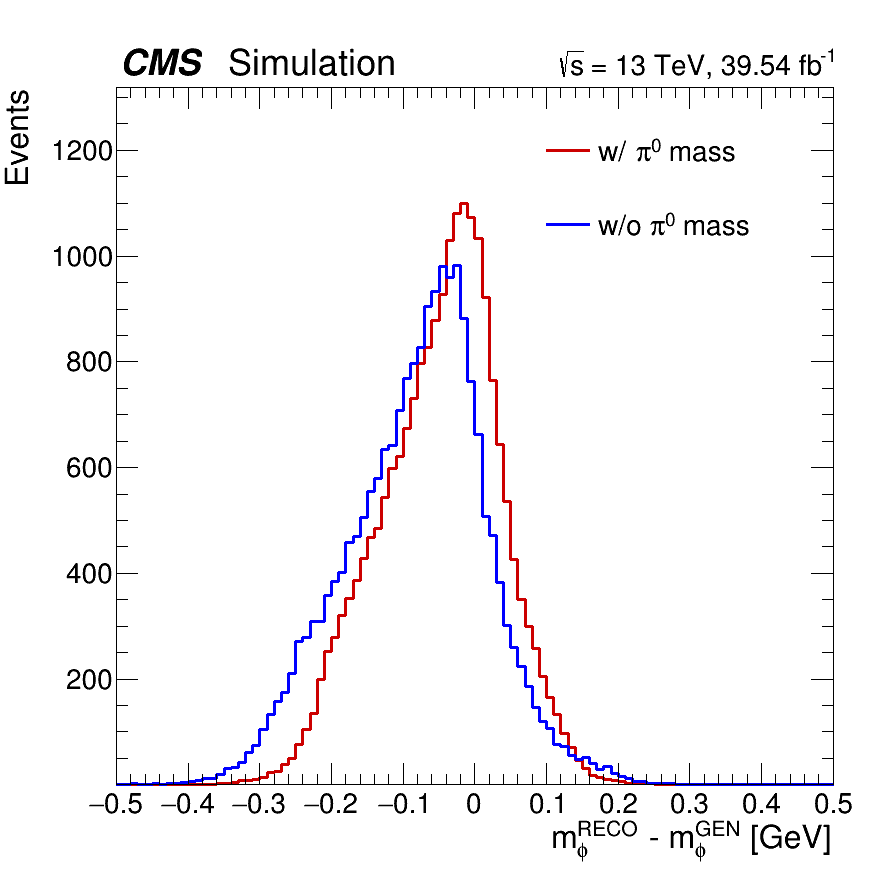
\includegraphics[width=0.49\mylength]{resources/plots/Phi3_fullmeson_mass_residual.png}
            \vspace*{-0.2cm}
            \caption{\footnotesize (a)}
    \end{subfigure}%
    \begin{subfigure}[t]{0.50\mylength}
            \centering
            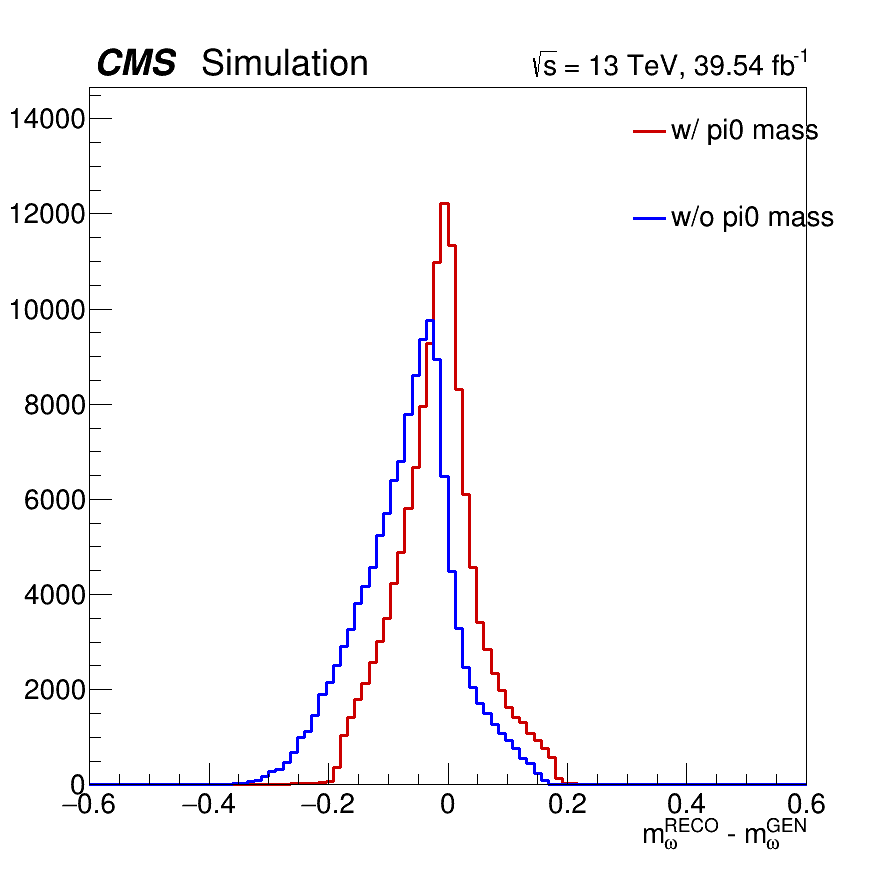
\includegraphics[width=0.49\mylength]{resources/plots/Omega_fullmeson_mass_residual.png}
            \vspace*{-0.2cm}
            \caption{\footnotesize (b)}
    \end{subfigure}%\begin{subfigure}[t]{0.50\mylength}\baselineski
    \caption{Full meson mass residuals for the different decay channels. (a) is for $\phi$, (b) is for $\omega$. The residuals shown in red are including the $\pi^0$ mass, and in blue without the correction.}
    \label{fig:full_meson_mass_residuals}
    \vspace*{-0.0cm}
\end{figure}

This slight improvement will enable us to narrow the selection cuts and reduce more background events, ultimately improving the final result. It will also contribute to the modelling of the signal, as explained in Section \ref{sec:modelling}, where the mass of the full meson will play a pivotal role.
\begin{table}[!ht]
    \centering
    \begin{tabular}{|l|c|C{3.2cm}@{}c|}
        \hline
        \cellcolor{lightgray}Decay channel & \cellcolor{lightgray}RMSE without $m_{\pi^0}$ correction& \multicolumn{2}{c|}{\cellcolor{lightgray}RMSE with $m_{\pi^0}$ correction} \\ \hline
        $\phi$          &98.7 MeV   &84.3 MeV  & (-15\%)   \\
        $\omega$        &100.7 MeV   &63.3 MeV  & (-37\%)   \\
        $\text{D}^{*0}$ 3-body &147.7 MeV   &127.8 MeV  & (-14\%)    \\
        \hline
        \end{tabular}
    \caption{Root mean squared errors with and without the $m_{\pi^0}$ correction for the $\phi$ and $\omega$ decay modes.}
    \label{tab:full_meson_mass_residuals_RMSE}
\end{table}

An additional correction was attempted. The idea was to reconstruct the neutral particle by summing the recovered photons, and then forcing the reconstructed neutral particle to have the $\pi^0$'s mass while maintaining the energy and direction ($\eta$ and $\phi$) unchanged. This required a slight modification of the neutral particle's transverse momenta, as given by
\begin{equation*}
    \pT = \sqrt{(E^2 - m^2)(1-\tanh^2\eta)}\ .
\end{equation*}
When adding this neutral particle to the ditrack, the full meson's $\pT$ remained effectively unchanged, and the full meson's mass was very similar (and slightly worse) compared to using the previous technique. Therefore, this adjustment was not used.

\subsection{Full meson transverse momentum}

To calculate the upper limits of the branching ratios of the decays, the Higgs boson invariant mass $m^{\text{H}}_{\gamma, M}$ is computed. This is done by extracting the mass component of the sum of the four momenta of the photon and the full meson. If $m^{\text{H}}_{\gamma, M}$ exhibits a narrow peak around the Higgs boson mass ($m_\text{H} = 125$ GeV), it is a strong indication that these particles were produced from the Higgs boson. To achieve a good resolution on $m^{\text{H}}_{\gamma, M}$, it is crucial to recover the two involved objects, i.e., the photon and the full meson, with utmost precision.

There are seven variables in play: the components of the four-momenta, four of which belong to the meson and three to the photon. The accuracy of the Higgs boson's invariant mass relies mainly on the accuracy of the transverse momenta of both particles involved. The other five variables ($\eta$ and $\phi$ of both particles and the mass of the full meson) are either already well measured or, in the case of the mass, too low in energy to significantly impact the computation. The corrections on the photon's transverse momentum of the photon are already discussed in Section \ref{subsec:photons}. Thus, the main emphasis should be on recovering the $\pT$ of the full meson as precisely as possible.
\begin{figure}[!ht]
    \captionsetup[subfigure]{labelformat=empty}
    \vspace*{-0.2cm}
    \centering
    \setlength{\mylength}{\textwidth}
    \begin{subfigure}[t]{0.50\mylength}
            \centering
            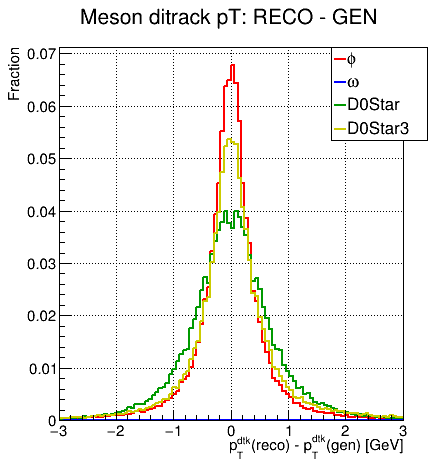
\includegraphics[width=0.49\mylength]{resources/plots/ditrack_residuals_pt.png}
            \vspace*{-0.2cm}
            \caption{\footnotesize (a)}
    \end{subfigure}%
    \begin{subfigure}[t]{0.50\mylength}
            \centering
            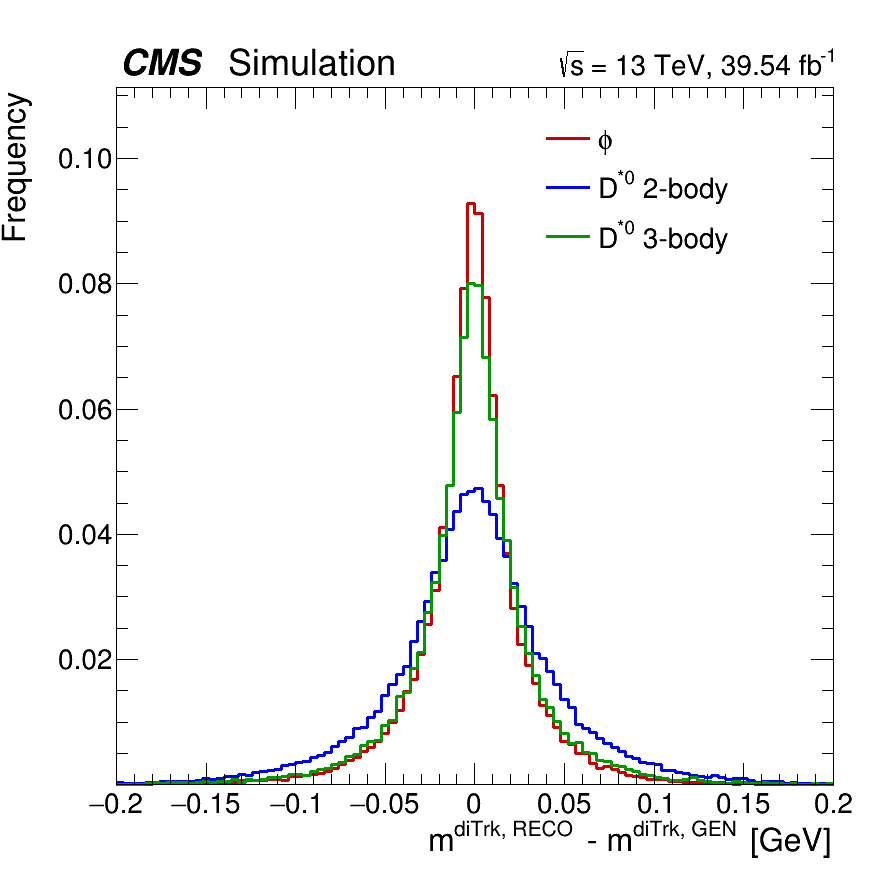
\includegraphics[width=0.49\mylength]{resources/plots/ditrack_residuals_mass.png}
            \vspace*{-0.2cm}
            \caption{\footnotesize (b)}
    \end{subfigure}%\begin{subfigure}[t]{0.50\mylength}\baselineskip
    \vskip\baselineskip
    \vspace*{-0.5cm}
    \begin{subfigure}[t]{0.50\mylength}
            \centering
            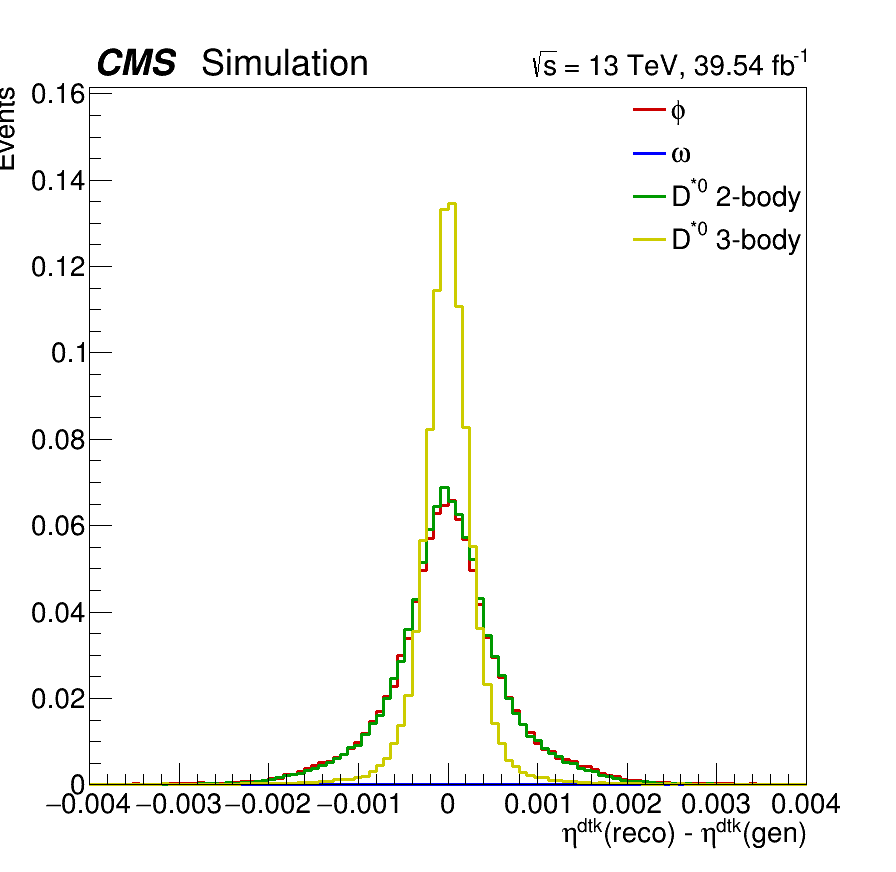
\includegraphics[width=0.49\mylength]{resources/plots/ditrack_residuals_eta.png}
            \vspace*{-0.2cm}
            \caption{\footnotesize (c)}
    \end{subfigure}%\begin{subfigure}[t]{0.50\mylength}
    \begin{subfigure}[t]{0.50\mylength}
            \centering
            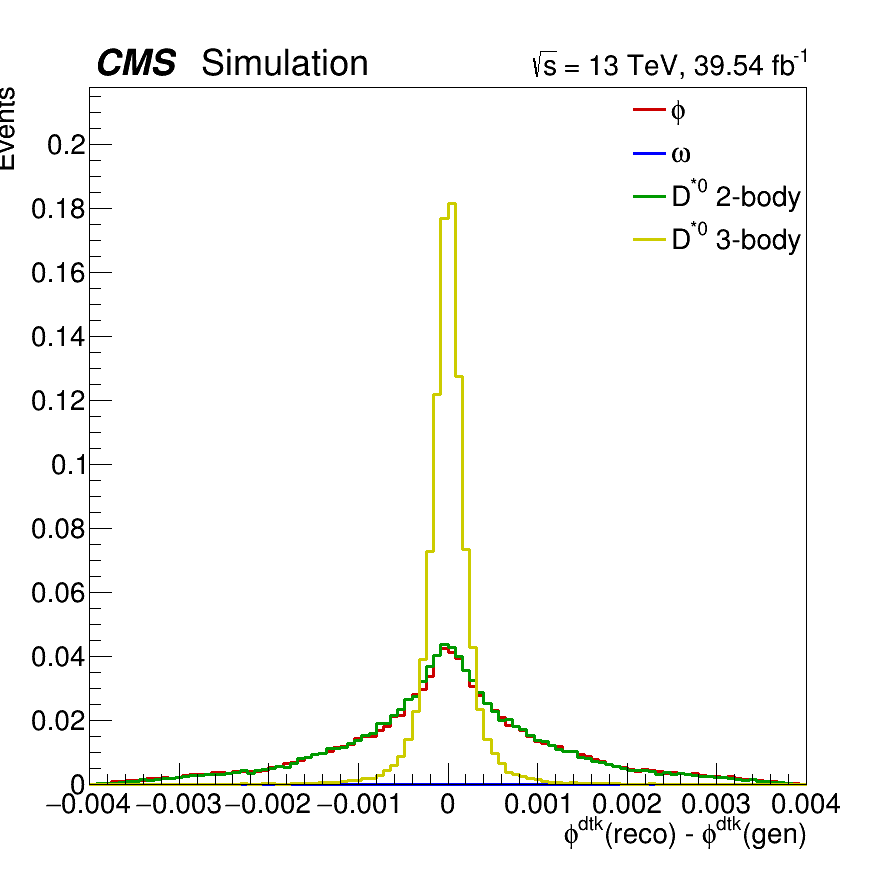
\includegraphics[width=0.49\mylength]{resources/plots/ditrack_residuals_phi.png}
            \vspace*{-0.2cm}
            \caption{\footnotesize (d)}
    \end{subfigure}%
    \vspace*{-0.0cm}
    \caption{Ditrack residuals for the different four-momentum components of each decay channel. (a) is for $\pT$, (b) is for the ditrack mass, (c) is for $\eta$, and (d) is for $\phi$. Three decay modes are shown: the $\phi$ in red, the D$^{*0}$ 2-body in blue, and the D$^{*0}$ 3-body in green. The $\omega$ ditrack residuals behave the same as the $\phi$ channel. All the residuals have been normalized to the same area to ease the comparison.}
    \label{fig:ditrack_residuals}
    \vspace*{-0.0cm}
\end{figure}

In each decay channel, the ditrack system variables are measured with remarkable accuracy. Figure \ref{fig:ditrack_residuals} displays the residuals of the ditrack transverse momentum, mass, $\eta$ and $\phi$ with respect to their generation-level MC value for every decay mode.

All histograms are normalized to the same area for comparing the various channels. It is worth noting that, as the ditrack consists of a pair of charged tracks that can be precisely determined thanks to the silicon tracker, the direction -- $\eta$ and $\phi$ -- is accurately measured for all channels.

The initial approach to reconstruct the full meson's transverse momentum is to sum the four-momenta of the ditrack system and those from the photons compatible with the decay of neutral particles. The main source of discrepancy between the full meson's transverse momenta and their generation-level MC values arises from the poorly reconstructed neutral particles. Given that the pions decay into softer photons that are hard to recover, many events exhibit missing energy, resulting in the full meson's $\pT$ being generally less energetic than expected. Figure \ref{fig:fullmeson_residuals_pt} shows the residuals of the full meson's transverse momentum with respect to their generation-level MC value for each decay mode.
\begin{figure}[!ht]
    \captionsetup[subfigure]{labelformat=empty}
    \vspace*{-0.2cm}
    \centering
    \setlength{\mylength}{\textwidth}
    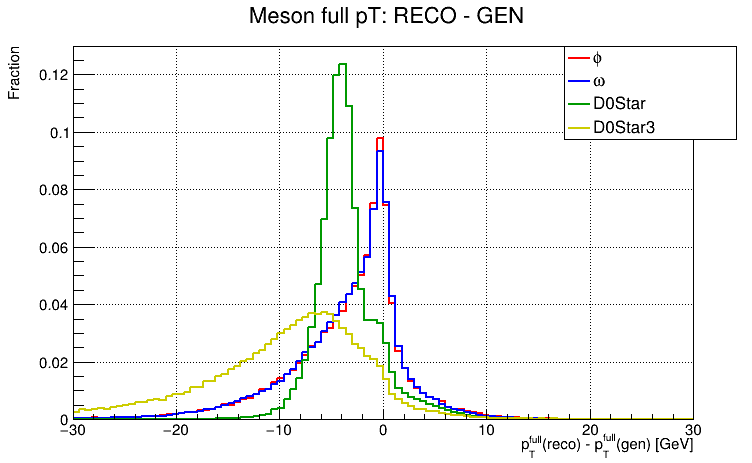
\includegraphics[width=0.49\mylength]{resources/plots/fullmeson_residuals_pt.png}
    \caption{Transverse momentum residuals for the full meson for each decay channel. All studied decay modes are shown: the $\phi$ in red, the $\omega$ in blue, the D$^{*0}$ 2-body in green, and the D$^{*0}$ 3-body in yellow. All the residuals have been normalized to the same area to ease the comparison.}
    \label{fig:fullmeson_residuals_pt}
    \vspace*{-0.0cm}
\end{figure}
Both the $\phi$ and $\omega$ channels exhibit an asymmetric left shoulder, consistent with the hypothesis of missing energy from the neutral particle. The $\text{D}^{*0}$ 2-body, on the other hand, is more symmetric but displaced about 5 GeV, since the soft $\pi^{0}/\gamma$ from $\text{D}^{*0}\decaysto \text{D}^{0}\pi^{0}/\gamma$ typically carries around $\sim5$ GeV in energy. The right shoulder results from events in which one photon compatible with this missing neutral particle is reconstructed, which is only around $\sim 13\%$ of events. The $\text{D}^{*0}$ 3-body combines characteristics from all previous channels, and since it is missing two neutral particles, it is noticeably shifted towards the lower end of the axis.

\subsection{\r BDTs to correct the full meson's momentum}

To address this issue, dedicated Boosted Decision Trees (BDTs) have been implemented for each channel using the Toolkit for Multivariate Data Analysis for \verb+ROOT+ \cite{CERN:root}, also known as \verb+TMVA+ \cite{TMVA:2007ngy}. This machine learning (ML) technique will correct for the full meson's $\pT$. A boosted decision tree is a ML binary classifier or regressor algorithm based on a flowchart-like structure in which each internal node represents a test on an attribute, each branch signifies the test's outcome, and each leaf node denotes a class level. For more detailed information, refer to Refs. \cite{TMVA:2007ngy, Coadou:2022nsh}.

The variables used in all models are presented in Table \ref{tab:model_variables}.
\begin{table}[!ht]
    \centering
    \begin{tabular}{|c|c|c|}
        \hline
        \multicolumn{3}{|c|}{\cellcolor{lightgray} Regression input variables} \\ \hline
        \cellcolor{lightgray}Dimensionless  &\cellcolor{lightgray}Dimensionful  &\cellcolor{lightgray}Normalised            \\\hline
        $\Delta R^{\gamma_1, \text{diTrk}}$             &$\pT^{\gamma_1}$           &$\pT^{\text{meson}}/\pT^{\gamma}$          \\
        $\Delta R^{\gamma_2, \text{diTrk}}$ ($^{*}$)   &$\pT^{\gamma_2}$ ($^{*}$) &$\pT^{\text{meson}}/\pT^{\text{diTrk}}$    \\
        $\eta^{\text{diTrk}}$                           &$m^{\text{diTrk}}$         &       \\
        $\Delta R^{\text{diTrk}}$                       &$m^{\text{meson}}$ ($^{**}$)  &       \\
        $\Delta(\eta^{\gamma_{\text{H}}}, \eta^{\text{diTrk}})$    & & \\
        $\Delta(\phi^{\gamma_{\text{H}}}, \phi^{\text{diTrk}})$    & & \\
        \hline
    \end{tabular}
    \caption{Input variables for the BDTs. $\gamma_1$ and $\gamma_2$ represent photons from neutral particle decay, $\gamma_{\text{H}}$ stands for the Higgs boson decay photon. The single asterisk denotes exclusion for the $\phi/\omega$ decay channels. The double asterisk denotes exclusion for the $\text{D}^{*0}$ 2-body decay channel.}
    \label{tab:model_variables}
\end{table}
The variables labelled by $\gamma_1$ and $\gamma_2$ refer to the recovered photons compatible with the decay of the neutral particles, while $\gamma_{\text{H}}$ refers to the photon originating in the Higgs boson decay. The dimensionless variables $\Delta R^{\gamma_1, \text{diTrk}}$ and $\Delta R^{\gamma_2, \text{diTrk}}$ reference the angular separation between each photon and the ditrack system. $\Delta R^{\text{diTrk}}$ is the angular separation within the track pair. It is worth defining $\Delta(\eta^{\gamma_{\text{H}}}, \eta^{\text{diTrk}})$ and $\Delta(\phi^{\gamma_{\text{H}}}, \phi^{\text{diTrk}})$,
\begin{equation*}
    \begin{aligned}
    \Delta(\eta^{\gamma_{\text{H}}}, \eta^{\text{diTrk}}) &= \eta^{\text{diTrk}} - \eta^{\gamma_{\text{H}}} \\
    \Delta(\phi^{\gamma_{\text{H}}}, \phi^{\text{diTrk}}) &= (\phi^{\text{diTrk}} - \phi^{\gamma_{\text{H}}}) \modu 2\pi \in[0, 2\pi)\ .
    \end{aligned}
\end{equation*}
The definition of $\Delta(\phi^{\gamma_{\text{H}}}, \phi^{\text{diTrk}})$ takes this form due to the periodic nature of the angular variable $\phi$. The single asterisk ($^{*}$) next to the variables related to the $\gamma_2$ indicates that they are not used for the $\phi/\omega$ decay channels, as the required selection criteria for these decay modes specify only one photon. Similarly, the double asterisk ($^{**}$) next to the full meson's mass indicates that this variable is not included for the $\text{D}^{*0}$ 2-body decay, as in this channel, $m^{\text{meson}}$ is not very precisely determined. The variables in Table \ref{tab:model_variables} have been selected after many model iterations, ensuring low correlation between them and with the Higgs boson invariant mass, while maintaining reasonable predictive power.

All the models have been trained to predict not the correct value of the full meson's transverse momentum, but a scale factor $\pT^{\text{meson, GEN}}/\pT^{\text{meson, RECO}}$ instead. This scale factor represents the adjustment needed for the reconstructed $\pT$ to match its generation-level MC value. The motivation for this approach is to avoid biasing the model by predicting a dimensionless variable.

We implemented the BDTs using the \verb+TMVA+ framework, specifically the
\begin{small}
\vspace*{-6pt}
\begin{verbatim}
TMVA::Factory.BookMethod(dataloader, TMVA::Types::kBDT, "modelName", "<options>");
\end{verbatim}
\vspace*{-6pt}
\end{small}
method, with the ML regressor \verb+TMVA::Types::kBDT+. To prevent overtraining, we employed cross-validation by rotating the training and testing samples. Specifically, the signal MC was divided into three subsets: A, B, and C. Three models with identical hyperparameters were trained on A+B (B+C / C+A) and tested on C (A / B). This approach ensures all the available data is used to train the models, while testing them on signal MC that was not used for training. To recover all the signal events, these three models were then applied to their respective testing subsets. Afterward, all the subsets were combined once more, resulting in a complete set of events.

\begin{figure}[!ht]
    \captionsetup[subfigure]{labelformat=empty}
    \vspace*{-0.2cm}
    \centering
    \setlength{\mylength}{\textwidth}
    \begin{subfigure}[t]{0.50\mylength}
        \centering
        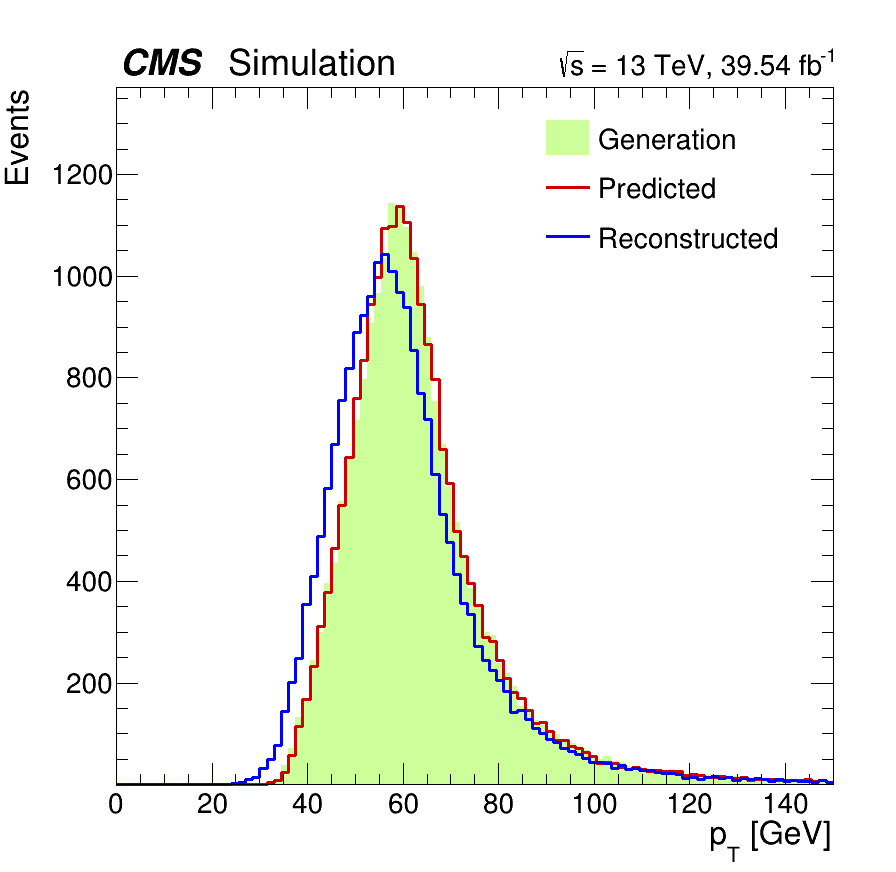
\includegraphics[width=0.49\mylength]{resources/plots/Phi3_model_pt.png}
        \vspace*{-0.2cm}
        \caption{\footnotesize (a)}
    \end{subfigure}%
    \begin{subfigure}[t]{0.50\mylength}
        \centering
        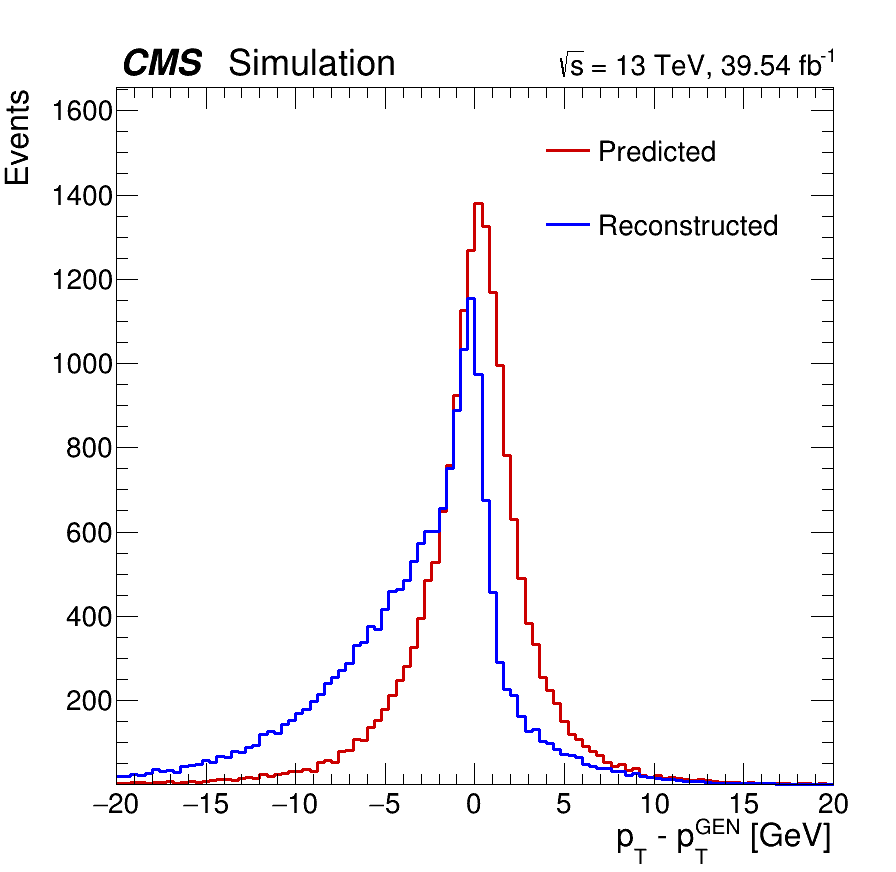
\includegraphics[width=0.49\mylength]{resources/plots/Phi3_model_pt_residuals.png}
        \vspace*{-0.2cm}
        \caption{\footnotesize (b)}
    \end{subfigure}%\begin{subfigure}[t]{0.50\mylength}\baselineskip
    \vskip\baselineskip
    \vspace*{-0.5cm}
    \begin{subfigure}[t]{0.50\mylength}
        \centering
        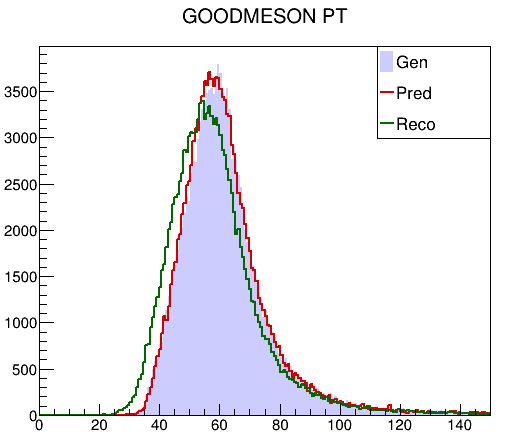
\includegraphics[width=0.49\mylength]{resources/plots/Omega_model_pt.png}
        \vspace*{-0.2cm}
        \caption{\footnotesize (c)}
    \end{subfigure}%
    \begin{subfigure}[t]{0.50\mylength}
        \centering
        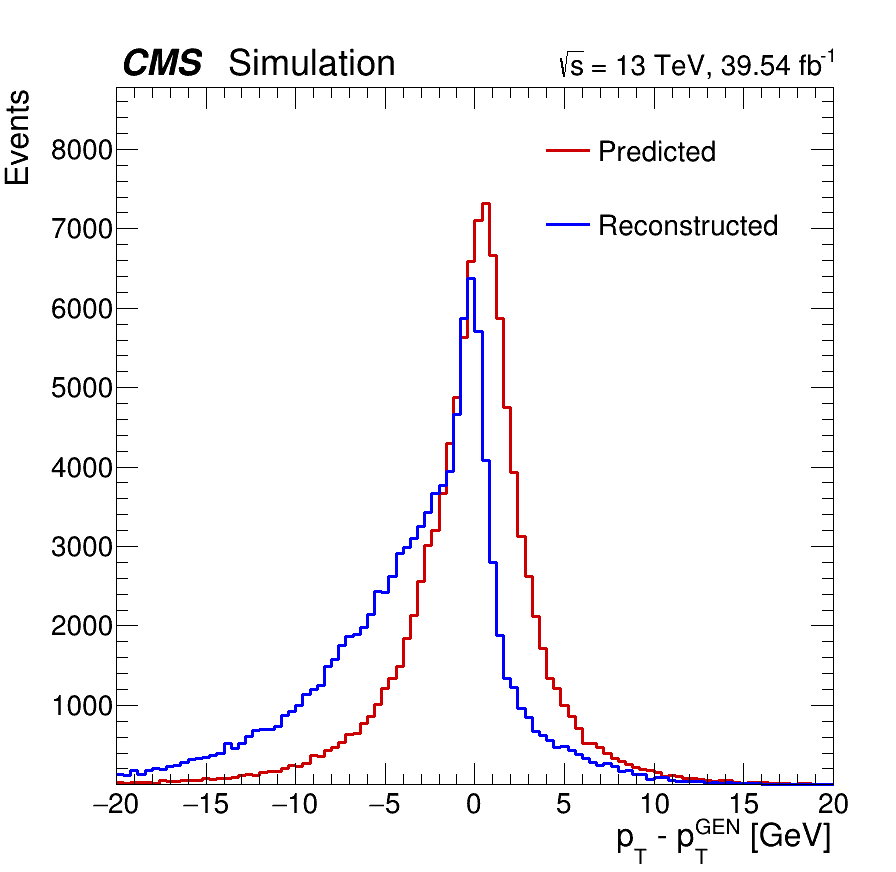
\includegraphics[width=0.49\mylength]{resources/plots/Omega_model_pt_residuals.png}
        \vspace*{-0.2cm}
        \caption{\footnotesize (d)}
    \end{subfigure}%\begin{subfigure}[t]{0.50\mylength}\baselineskip
\caption{Transverse momentum of the $\phi$ and $\omega$ mesons. (a/c) Display the generation-level MC transverse momenta in green, the prediction by the BDT in red, and the recovery by the initial approach in blue, for the $\phi/\omega$ mesons, respectively. (b/d) Show the residuals with (red) and without (green) the BDT prediction, for the $\phi/\omega$ mesons, respectively.}
\label{fig:pt_residuals_model_omega_phi}
    \vspace*{-0.0cm}
\end{figure}

The hyperparameters for each model are available in Table \ref{tab:hyperparameters_models} in the Appendix. Figures \ref{fig:pt_residuals_model_omega_phi} and \ref{fig:pt_residuals_model_d0star} compare the generation-level MC transverse momentum with the reconstruction values, both with and without regression, and show the residuals for each channel.
\begin{figure}[!ht]
    \captionsetup[subfigure]{labelformat=empty}
    \vspace*{-0.2cm}
    \centering
    \setlength{\mylength}{\textwidth}
    \begin{subfigure}[t]{0.50\mylength}
        \centering
        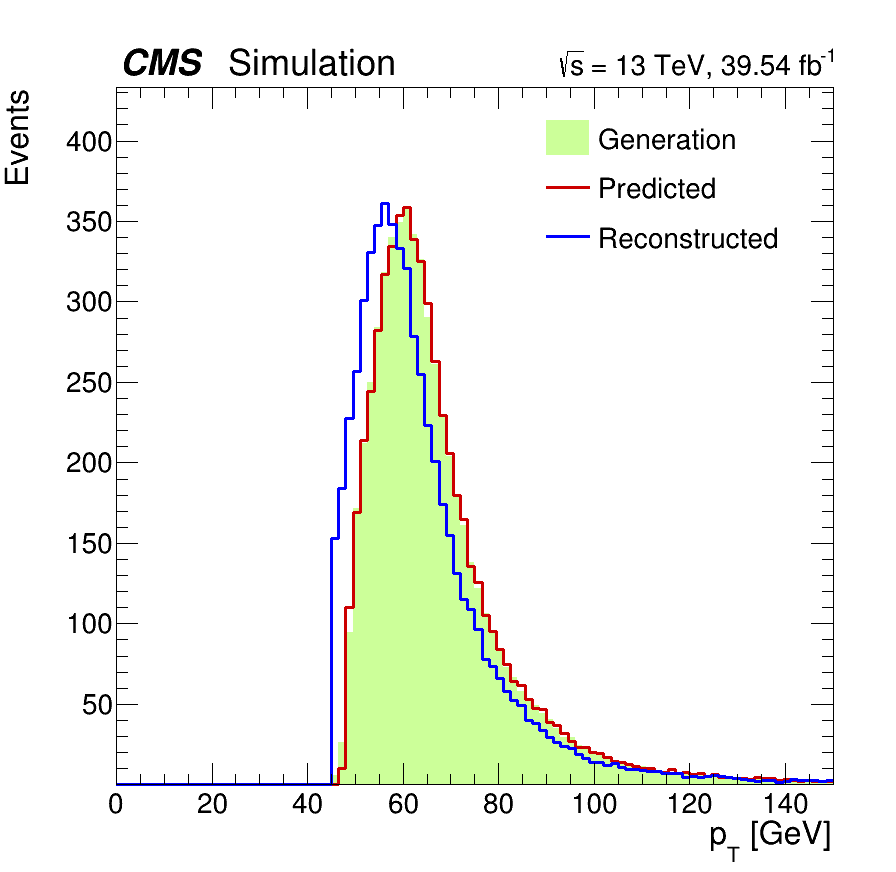
\includegraphics[width=0.49\mylength]{resources/plots/D0Star_2body_model_pt.png}
        \vspace*{-0.2cm}
        \caption{\footnotesize (a)}
    \end{subfigure}%
    \begin{subfigure}[t]{0.50\mylength}
        \centering
        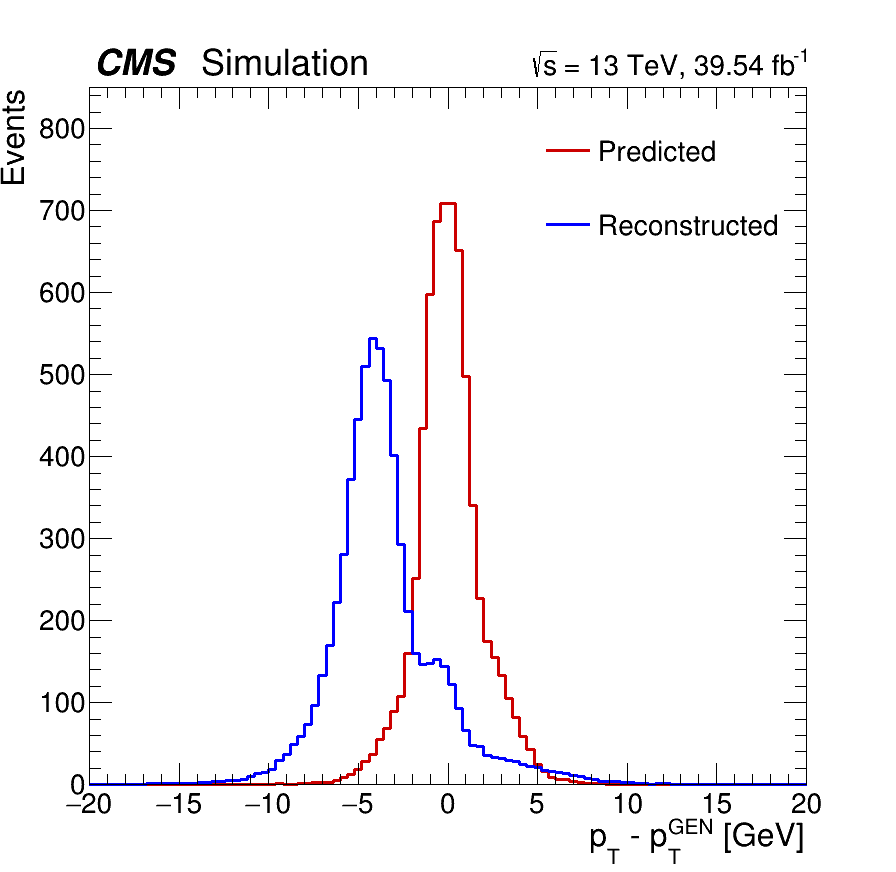
\includegraphics[width=0.49\mylength]{resources/plots/D0Star_2body_model_pt_residuals.png}
        \vspace*{-0.2cm}
        \caption{\footnotesize (b)}
    \end{subfigure}%\begin{subfigure}[t]{0.50\mylength}\baselineskip
    \vskip\baselineskip
    \vspace*{-0.5cm}
    \begin{subfigure}[t]{0.50\mylength}
        \centering
        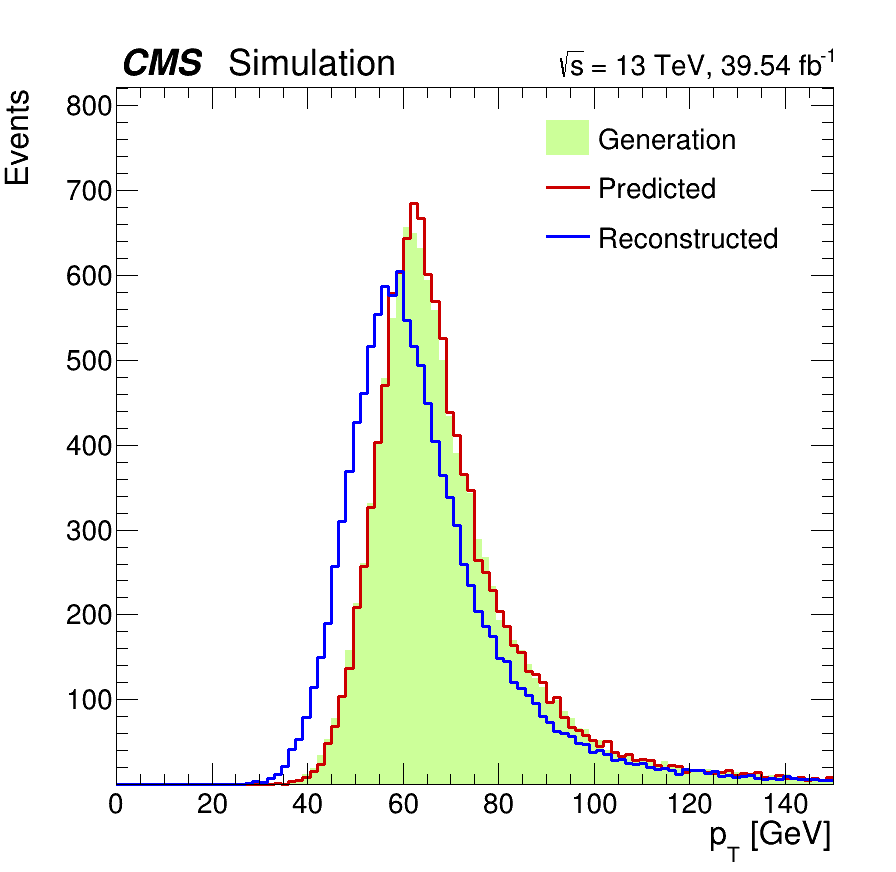
\includegraphics[width=0.49\mylength]{resources/plots/D0Star_3body_model_pt.png}
        \vspace*{-0.2cm}
        \caption{\footnotesize (c)}
    \end{subfigure}%
    \begin{subfigure}[t]{0.50\mylength}
        \centering
        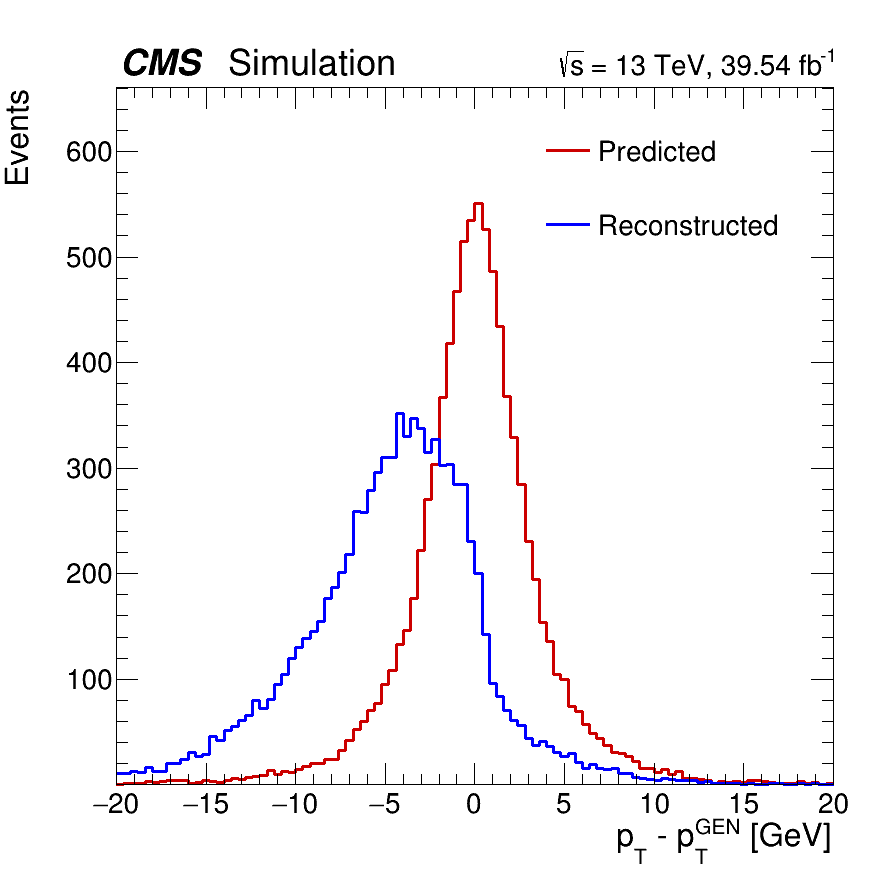
\includegraphics[width=0.49\mylength]{resources/plots/D0Star_3body_model_pt_residuals.png}
        \vspace*{-0.2cm}
        \caption{\footnotesize (d)}
    \end{subfigure}%\begin{subfigure}[t]{0.50\mylength}\baselineskip
\caption{Transverse momentum of the $\text{D}^{*0}$ meson in both the 2-body and 3-body decay channels. (a/c) Display the generation-level MC transverse momenta in green, the prediction by the BDT in red, and the recovery by the initial approach in blue, for the 2/3-body decay channel, respectively. (b/d) Show the residuals with (red) and without (green) the BDT prediction, for the 2/3-body decay channel, respectively.}
\label{fig:pt_residuals_model_d0star}
    \vspace*{-0.0cm}
\end{figure}

Both $\phi$/$\omega$ channels displayed in Figure \ref{fig:pt_residuals_model_omega_phi} are quite similar. For both full mesons, the predicted transverse momentum spectrum aligns well with the generation-level one. Additionally, the residuals for the predicted values are centred around the origin and symmetric, indicating that the predicted $\pT$ no longer exhibits missing energy. They are also higher around the origin than the reconstructed residuals, meaning that the predicted values are closer to the generation-level ones than the reconstructed $\pT$'s. The 2-body decay channel presented in Figure \ref{fig:pt_residuals_model_d0star} shows that the model accurately shifts the full meson transverse momentum by around 5 GeV, as the residuals are narrow around 0 GeV instead of around -5 GeV, and it is also more symmetric than the initially reconstructed $\pT$. The 3-body decay channel shown in Figure \ref{fig:pt_residuals_model_d0star} has the poorest transverse momentum reconstruction before the BDT, but shows a significant improvement after applying the regression. Similar to the other channels, the residuals are centred, symmetric and with a higher maximum near the origin.

Table \ref{tab:models_pt_RMSE} quantifies these improvements and shows the root mean squared errors with respect to generation-level transverse momentum, both with and without the BDT regression, for each channel. Applying the transverse momenta regression noticeably improves the $\pT$ values and reduces the error for all channels by around 20\% - 40\%.
\begin{table}[!ht]
    \centering
    \begin{tabular}{|l|c|C{3.1cm}@{}c|}
        \hline
        \cellcolor{lightgray}Decay channel & \cellcolor{lightgray}RMSE without $\pT$ regression & \multicolumn{2}{c|}{\cellcolor{lightgray}RMSE with $\pT$ regression} \\ \hline
        $\phi$          &4.900 GeV   &3.580 GeV  & (-27\%)  \\
        $\omega$        &5.029 GeV   &4.038 GeV  & (-20\%)  \\
        $\text{D}^{*0}$ 2-body &3.170 GeV   &1.897 GeV  & (-40\%)  \\
        $\text{D}^{*0}$ 3-body &5.126 GeV   &3.711 GeV  & (-28\%)  \\
        \hline
        \end{tabular}
    \caption{Root mean squared errors of the full meson's transverse momentum with and without the BDT regression for each decay mode.}
    \label{tab:models_pt_RMSE}
\end{table}
The applied BDTs not only significantly reduce the error in the transverse momentum of the full meson for every channel but also restore the symmetric residual shape of the variable. This indicates that the estimated $\pT$ values are as likely to be underestimated as to be overestimated, accounting for the missing energy from the undetected neutral particles. This reduction in the width of the residuals will directly lead to an improved, lower upper limit on the Higgs boson branching fraction.

A crucial consideration in developing any ML model is overtraining, and this case is no exception. This is the primary reason a dimensionless scale factor was predicted rather than the direct value of the momentum. In this situation, overtraining can be directly detected by examining the background shape after applying the regression. If the model learns that, regardless of the input, the predicted value should lead to a peak around 125 GeV when constructing the Higgs invariant mass variable, we know it is overtrained and biased and needs to be rejected. To address this potential issue, a \textit{background shaping function (BSF)} was introduced, providing a dimensionless metric that increases as the model becomes more biased. The developed BSF for measuring each model is defined to be
\begin{equation*}
    BSF \propto -A\log{(\mu-125)^2} + B N + C \sqrt{b}\ ,
\end{equation*}
where $A$, $B$, and $C$ are constants, $\mu$ is the peak of a fitted double-sided Crystal Ball\footnote{A double-sided Crystal Ball function, named after the Crystal Ball Collaboration \cite{A2:CB}, is a probability density function (PDF) commonly used in high-energy physics (HEP). It is built from a Gaussian centre and two asymmetric tails modelled by power-law functions. Additional details about this PDF and its implementation in \verb+ROOT+ can be found in Ref. \cite{CERN:root_CB}.} (CB) to the Higgs boson's invariant mass constructed from background MC events, $N$ is the normalization constant of the Crystal Ball, and $b$ is the number of events in the interval $(117, 133)$ GeV of the Higgs boson's invariant mass. Note that the BSF depends only on background events, more particularly in reconstructing the Higgs boson's invariant mass. The first factor penalizes the model more when the background Higgs boson's invariant mass shape peaks around $m_\text{H}=125\ \GeV$, because the background should be flat or asymptotically falling near that value. The remaining two factors account for the number of background events near the expected signal peak. More background events result in a smaller and thus worse signal-to-background ratio, a quantity to maximize for improving the computation of upper limits.

Figure \ref{fig:BSF_vs_RMSE_phi} shows the BSF as a function of the RMSE of different models applied to reconstruct the transverse momentum of the $\phi$ meson.
\begin{figure}[!ht]
    \captionsetup[subfigure]{labelformat=empty}
    \vspace*{-0.2cm}
    \centering
    \setlength{\mylength}{\textwidth}
    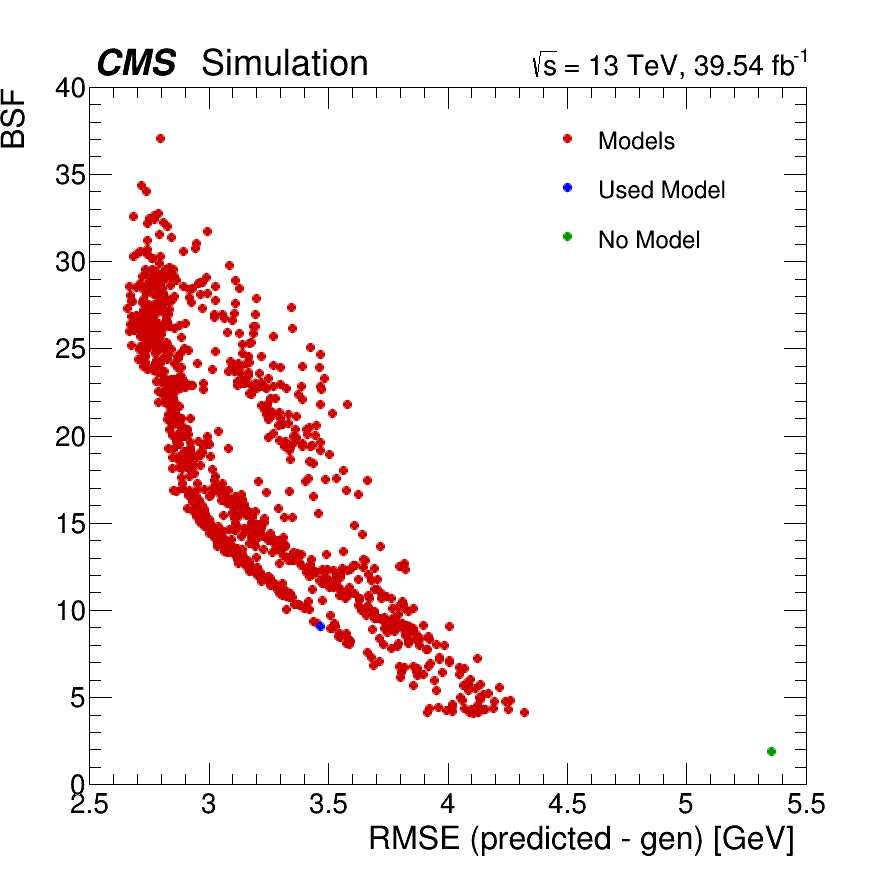
\includegraphics[width=0.49\mylength]{resources/plots/BSF_vs_RMSE_phi.png}
    \caption{Background shaping function (BSF) as a function of the root mean squared error (RMSE) of the $\pT$ for various models of the $\phi$ decay channel. The reconstructed and the explored and used model's values are shown in blue, green and red, respectively. The explored models follow an expected trend: as the BSF increases (the model becomes more biased), the RMSE decreases, a sign of overtraining.}
    \label{fig:BSF_vs_RMSE_phi}
    \vspace*{-0.0cm}
\end{figure}
The studied models follow an expected trend: as the BSF increases, and consequently, the model becomes more biased, the RMSE decreases. All decay channels have a similar behaviour, so only the $\phi$ channel is shown. To select one model from the many tens of thousands that were tested, compromises must be made, as there is a trade-off between not shaping the background and significantly improving the error. Different BSF thresholds for each decay channel were identified, considering that each decay involves a different number of events, directly related to the BSF values. Thus, it is not meaningful to compare BSF values across channels; it is only relevant to compare them within a single channel. For the $\phi$ decay channel, a value of around 8 was found to be optimal by directly examining the shape of the background Higgs boson's invariant mass.

\subsection{Meson selection criteria}\label{subsec:meson_selection}

After having presented all the techniques for reconstructing the meson, some selection cuts can be applied. These aim to preserve the maximum number of signal events while rejecting as many background events. Tables \ref{tab:meson_selection_1} and \ref{tab:meson_selection_2} summarize the meson candidate selection criteria used for each decay channel, where $\gamma^{\text{diTrk}}$ are the photons from neutral particle decays, and $\gamma_\text{H}$ refers to the photon originating from the Higgs boson decay.
\begin{table}[!ht]
    \centering
    \begin{tabular}{|l|c|c|}
        \hline
        \cellcolor{lightgray}Variable & \cellcolor{lightgray}$\phi(\pi^{\pm}\pi^{\mp}\pi^{0})$ & \cellcolor{lightgray}$\omega(\pi^{\pm}\pi^{\mp}\pi^{0})$ \\ \hline
        Meson mass                                              &$0.80-1.15$ GeV  &$0.60-0.90$ GeV    \\
        Ditrack mass                                            &$0.34-0.84$ GeV  &$0.32-0.62$ GeV      \\
        $\pT^{\text{diTrk}}$                                    &$>15$ GeV        &$>20$ GeV              \\
        $\pT^{\text{leadTrk}}$                                  &$>12$ GeV        &$>12$ GeV               \\
        $\pT^{\text{subLeadTrk}}$                               &$>3$ GeV         &$>3$ GeV           \\
        $\#\gamma^{\text{diTrk}}$                               &$>0$             &$>0$                   \\
        $\Delta(\phi^{\text{diTrk}}, \phi^{\gamma_\text{H}})$   &$\pi\pm2.3$      &$\pi\pm2.3$        \\
        $\Delta(\eta^{\text{diTrk}}, \eta^{\gamma_\text{H}})$   &$0\pm1.9$        &$0\pm1.9$              \\
        Iso                                                     &$>0.95$          &$>0.95$                \\
        \hline
        \end{tabular}
    \caption{Selection criteria applied to the $\phi$ and $\omega$ mesons used in the analysis.}
    \label{tab:meson_selection_1}
\end{table}

\begin{table}[!ht]
    \centering
    \begin{tabular}{|l|c|c|}
        \hline
        \cellcolor{lightgray}Variable & \cellcolor{lightgray}$\text{D}^{*0}(\text{K}^{-}\pi^{+}{\scriptstyle(\pi^{0}/\gamma)})$ & \cellcolor{lightgray}$\text{D}^{*0}(\text{K}^{-}\pi^{+}\pi^{0}{\scriptstyle(\pi^{0}/\gamma)})$ \\ \hline
        Meson mass                                              &                   &$1.50-2.10$ GeV  \\
        Ditrack mass                                            &$1.805-1.925$ GeV  &$0.65-1.70$ GeV  \\
        $\pT^{\text{diTrk}}$                                    &$>42$ GeV          &$>20$ GeV           \\
        $\pT^{\text{leadTrk}}$                                  &$>22$ GeV          &$>12$ GeV           \\
        $\pT^{\text{subLeadTrk}}$                               &$>10$ GeV          &$>3$ GeV           \\
        $\#\gamma^{\text{diTrk}}$                               &                   &$>0$               \\
        $\Delta(\phi^{\text{diTrk}}, \phi^{\gamma_\text{H}})$   &$\pi\pm2.3$        &$\pi\pm2.3$        \\
        $\Delta(\eta^{\text{diTrk}}, \eta^{\gamma_\text{H}})$   &$0\pm1.9$          &$0\pm1.9$           \\
        Iso                                                     &$>0.90$            &$>0.95$             \\
        \hline
        \end{tabular}
    \caption{Selection criteria applied to each channel of the $\text{D}^{*0}$ meson decay used in the analysis.}
    \label{tab:meson_selection_2}
\end{table}

In most of the events the full meson and the photon are back-to-back, so $\Delta(\phi^{\text{diTrk}}, \phi^{\gamma_\text{H}})$ is centred around $\pi$. We select highly isolated particles as this significantly reduces background contribution.

\section{Event selection}\label{sec:event_selection}

The analysis described here searches for the Higgs boson decaying to a photon and to either a $\phi$, $\omega$ or $\text{D}^{*0}$ meson. The signal features narrow peaks in the ditrack's mass (for the $\text{D}^{*0}$ 2-body decay), the full meson's mass (for the $\phi$, $\omega$ and $\text{D}^{*0}$ 3-body decays), and the photon-meson invariant mass $m^{\text{H}}_{\gamma, M}$ distributions over the SM backgrounds. These resonances can be fully reconstructed thanks to the excellent resolution of the CMS detector in measuring of the photon energy and track momentum. Nevertheless, the accuracy of these three-body decays is not as good as in other exotic Higgs boson decays of the same type, but where the vector meson decays only into a pair of charged tracks.

The $\phi\gamma$, $\omega\gamma$ and $\text{D}^{*0}\gamma$ exclusive final states are very similar. Meson candidates are paired with photon candidates to form $M\gamma$ candidates. When multiple photon candidates meeting the selection criteria outlined in Section \ref{sec:objects} are present, the one with the highest transverse momentum is chosen. Similarly, when multiple meson candidates satisfying the selection criteria described in Section \ref{subsec:meson_selection} are found, the one with a mass closest to the theoretical mass value of the meson is chosen.

The $\phi\gamma$ and $\omega\gamma$ channels in particular closely resemble each other, both decaying into $\pi^{+}\pi^{-}\pi^0$ and having similar masses and decay widths. The $\text{D}^{*0}$ 2-body decay can effectively be treated as a three-body decay, $\text{D}^{*0}\decaysto \text{K}^{-}\pi^{+}\pi^0/\gamma$, due to its short lifetime. The main difference between this channel and the $\phi/\omega$ channel is that in the $\phi/\omega$ case, the three pions carry, on average, approximately the same energy, while for $\text{D}^{*0}$ the neutral particle is very soft, carrying only around 5 GeV. Finally, the $\text{D}^{*0}$ 3-body decay can effectively be treated as a 4-body decay for the same reason, with 2 charged tracks, one soft neutral particle, and one neutral pion. This last case shares similarities with the previous ones.

To reduce the number of background events while maintaining a lot of events from ggH and VBF, only the lepton veto was applied, discarding events with additional charged leptons with $\pT$ > 10 GeV.% Events with two or more jets having $\pT$ > 30 GeV and $\abs{\eta} < 4.7$, exhibiting a significant pseudorapidity gap ($\abs{\Delta\eta_{jj}} > 3$), and with an invariant mass $m_{jj} > 300\ \GeV$, are excluded from this category. Jets should not overlap with the meson and photon forming the Higgs boson candidate and must meet the criteria mentioned in Section \ref{sec:objects}.
% Table \ref{tab:triggers} summarizes the selection criteria for this production mode, which must additionally satisfy the selection rules of the tau-like trigger described in Section \ref{subsec:data_tau_trigger}.
%\begin{table}[!ht]
%    \centering
%    \begin{tabular}{|c|c|c|c|}
%    \hline
%    \cellcolor{lightgray}Target signal   & \cellcolor{lightgray}Trigger & \cellcolor{lightgray}Selection & \cellcolor{lightgray}Integrated luminosity (fb$^{-1}$)\\ \hline
%    \multirow{1}{*}{ggH}&\multirow{1}{*}{tau-like}  &no e/$\mu$ with $\pT$ > 10 GeV & \multirow{1}{*}{39.54 (2018)}\\
%    \hline
%    \end{tabular}
%    \caption{Selection criteria used for the ggH production mode, alongside the integrated luminosity provided by CMS compatible with these criteria.}
%    \label{tab:triggers}
%\end{table}

Table \ref{tab:selection_efficiency} reports the signal cut flow. The product of signal selection efficiency and acceptance ($\epsilon$A) corresponds to the fraction of MC simulated signal events that pass the selection.
\begin{table}[!ht]
    \centering
    \begin{tabular}{|c|c|c|c|c|}
        \hline
        \cellcolor{lightgray}Selection &\cellcolor{lightgray}$\text{H}\decaysto \phi\gamma$ &\cellcolor{lightgray}$\text{H}\decaysto \omega\gamma$ &\cellcolor{lightgray}$\text{H}\decaysto D^{*0}\gamma$ {\scriptsize(2-body)}&\cellcolor{lightgray}$\text{H}\decaysto D^{*0}\gamma$ {\scriptsize(3-body)}\\ \hline
        trigger                                     & 24\%  & 23\%  & 17\%  & 19\% \\
        1 good $\gamma$                             & 89\%  & 90\%  & 89\%  & 90\% \\
        1 good meson                                & 33\%  & 36\%  & 55\%  & 25\% \\
        0 leptons                                   & 99\%  & 98\%  & 99\%  & 99\% \\ \hline
        Cumulative $\epsilon$A                      & 7.0\%  & 7.4\%  & 8.2\%  & 4.2\% \\
        \hline
        \end{tabular}
    \caption{Signal selection efficiency for all decay channels.}
    \label{tab:selection_efficiency}
\end{table}
The efficiencies for the $\phi$ and $\omega$ channels are consistently similar throughout the selection flow. It can be observed that the high-level trigger is less efficient for the $\text{D}^{*0}$ decay mode compared to the other channels, resulting in a lower cumulative acceptance.

These strict cuts (selecting approximately only one in eleven signal events) will eliminate most of the background events, which for the ggH enriched channel, it dominantly consists of $\gamma$ + multijet process, with a smaller contribution arising from QCD multijet. The 2-body $\text{D}^{*0}$ decay is expected to have less background compared to the $\phi$, $\omega$ and 3-body $\text{D}^{*0}$ decays, as in the 2-body case the very well-measured ditrack is a real resonance with a narrow width. Additionally, the $\omega$ channel is expected to have also less background than the $\phi$ and 3-body $\text{D}^{*0}$ decays due to its sharper decay width.

\section{MC-data comparison}

This section will provide a comparison between the signal MC, the background MC, and real data of the most important kinematic variables involved in these processes. The MC signal in all figures has been normalized to the same area as the data to improve the visualization. Each figure also provides the ratio between data and MC background, which consists of $\gamma$ + jets. In all plots, the MC background underestimates the data as it only considers the dominant contribution (i.e., $\gamma$ + jets) at LO, and thus the number of background events from real data is a factor of around 30\% larger than MC. This is not a concern, since the estimated limits are ultimately calculated using the data for the background fit. The MC background serves the purpose of helping us comprehend the behaviour of the involved processes.

Figure \ref{fig:ditrack_mass_data} displays the invariant mass of the ditrack system. For the $\phi$, $\omega$ and D$^{*0}$ 3-body decay channels, depicted in Figure \ref{fig:ditrack_mass_data} (a), (b), and (d), respectively, the ditrack mass is very wide, since the ditrack system does not form a real particle. In contrast, the ditrack mass for the D$^{*0}$ 2-body decay channel, shown in Figure \ref{fig:ditrack_mass_data} (c), exhibits a sharper resonance around 1.86 GeV. This is because in this case, the ditrack system is a real $\text{D}^{0}$ meson. This distinctive feature will be exploited when modelling the signal. Moreover, it is seen that the MC background is consistent with the data across all decay modes.
\begin{figure}[!ht]
    \captionsetup[subfigure]{labelformat=empty}
    \vspace*{-0.2cm}
    \centering
    \setlength{\mylength}{\textwidth}
    \begin{subfigure}[t]{0.50\mylength}
        \centering
        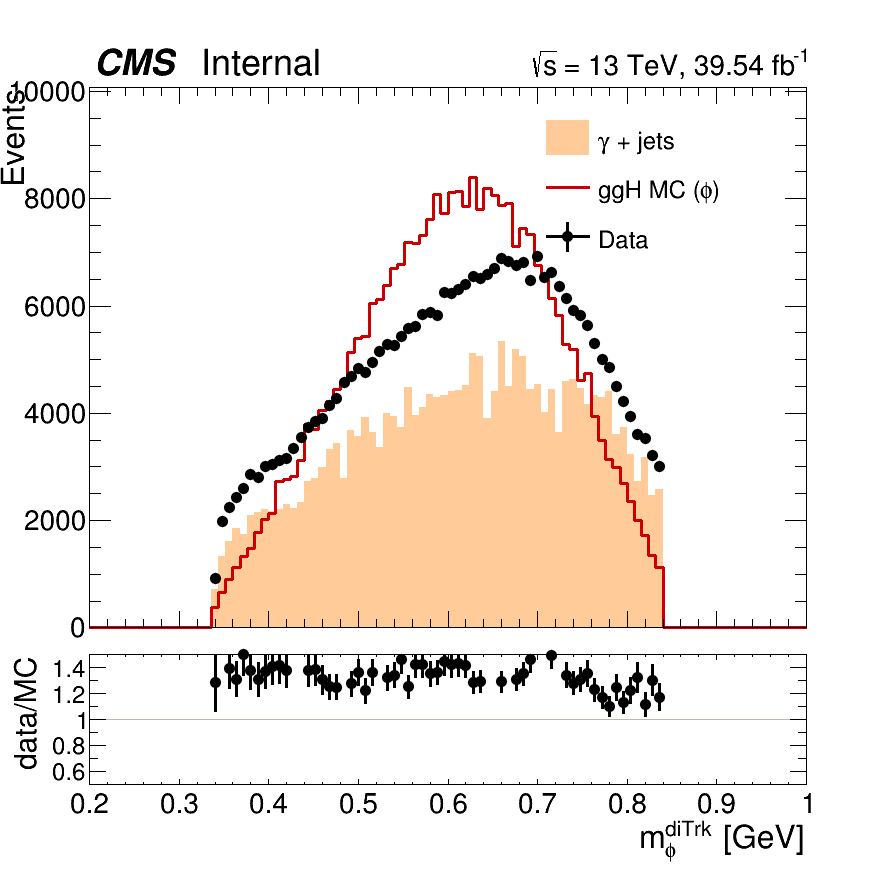
\includegraphics[width=0.49\mylength]{resources/plots/Phi3_ditrk_mass.png}
        \vspace*{-0.2cm}
        \caption{\footnotesize (a)}
    \end{subfigure}%
    \begin{subfigure}[t]{0.50\mylength}
        \centering
        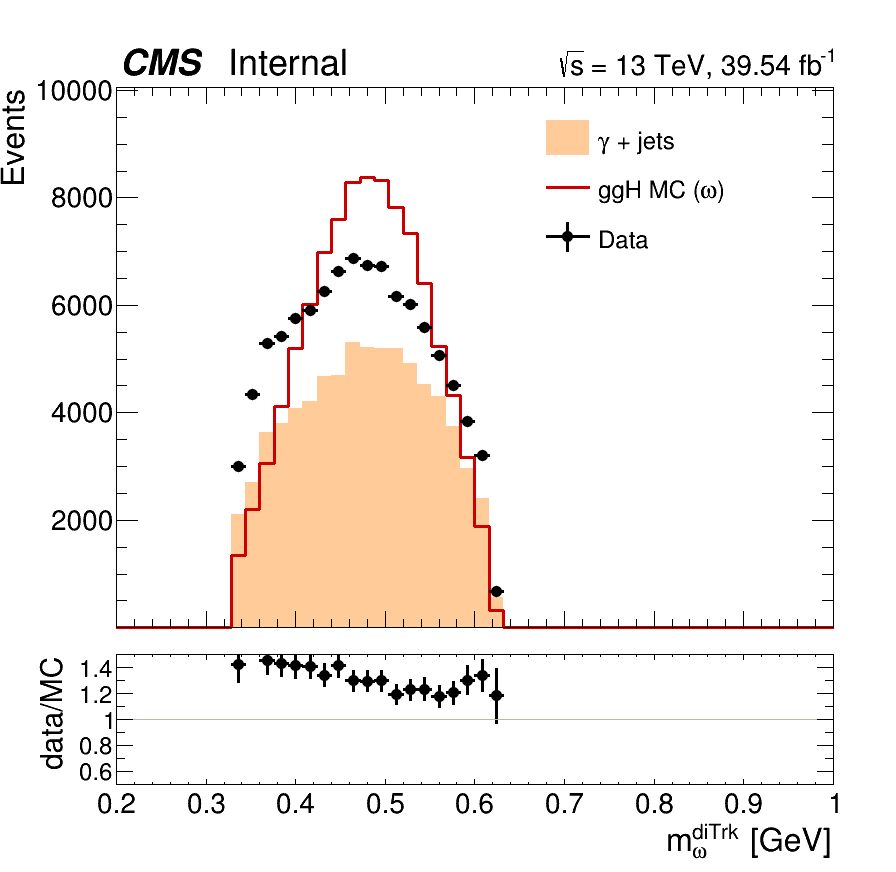
\includegraphics[width=0.49\mylength]{resources/plots/Omega_ditrk_mass.png}
        \vspace*{-0.2cm}
        \caption{\footnotesize (b)}
    \end{subfigure}%\begin{subfigure}[t]{0.50\mylength}\baselineskip
    \vskip\baselineskip
    \vspace*{-0.5cm}
    \begin{subfigure}[t]{0.50\mylength}
        \centering
        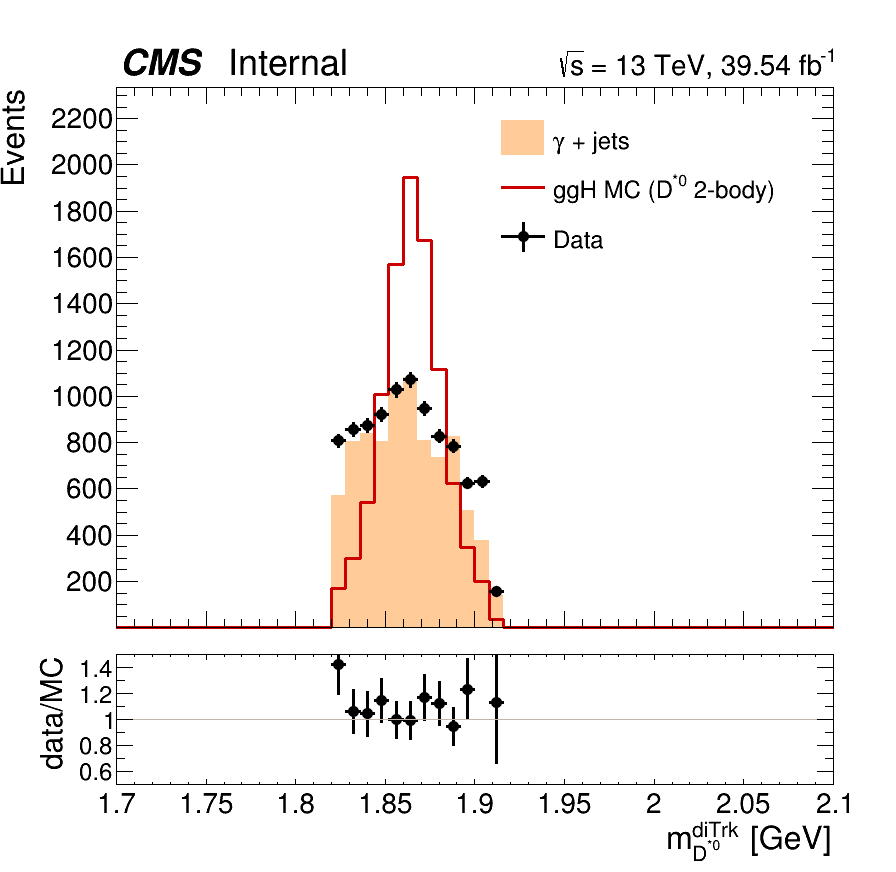
\includegraphics[width=0.49\mylength]{resources/plots/D0Star_2body_ditrk_mass.png}
        \vspace*{-0.2cm}
        \caption{\footnotesize (c)}
    \end{subfigure}%
    \begin{subfigure}[t]{0.50\mylength}
        \centering
        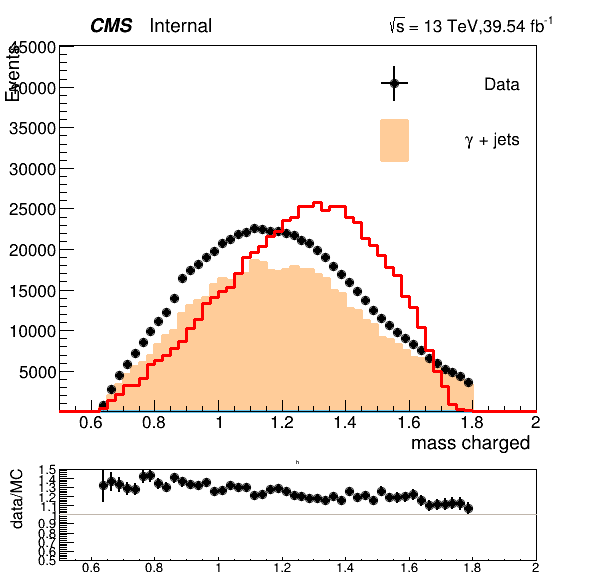
\includegraphics[width=0.49\mylength]{resources/plots/D0Star_3body_ditrk_mass.png}
        \vspace*{-0.2cm}
        \caption{\footnotesize (d)}
    \end{subfigure}%\begin{subfigure}[t]{0.50\mylength}\baselineskip
\caption{Ditrack mass of the different studied decay modes. (a) $\phi$ channel, (b) $\omega$ channel, (c) $\text{D}^{*0}$ 2-body channel, and (d) $\text{D}^{*0}$ 3-body channel. The MC background is shown in orange, scatter points represent real data, and the signal, in red, is normalized to the data for better visualization.}
\label{fig:ditrack_mass_data}
    \vspace*{-0.0cm}
\end{figure}

\newpage

Figure \ref{fig:full_mass_data} displays the mass of the full meson. This variable is sharper than the ditrack system's mass in all channels because it consists of a real meson. However, for the $\text{D}^{*0}$ 2-body decay mode, it is not well reconstructed.
\begin{figure}[!ht]
    \captionsetup[subfigure]{labelformat=empty}
    \vspace*{-0.2cm}
    \centering
    \setlength{\mylength}{\textwidth}
    \begin{subfigure}[t]{0.50\mylength}
        \centering
        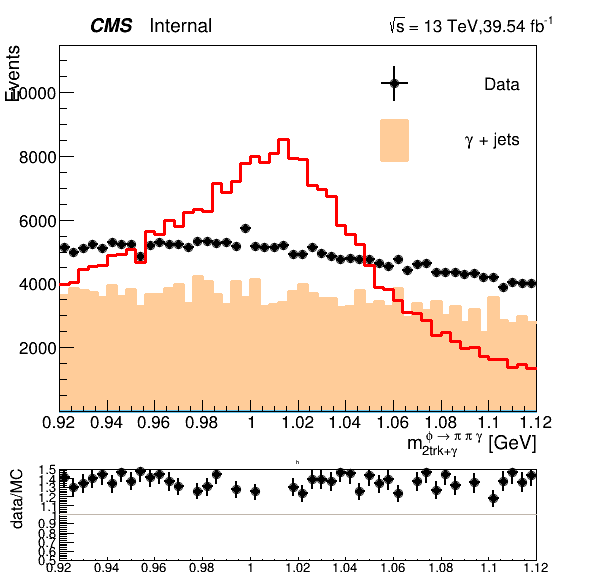
\includegraphics[width=0.49\mylength]{resources/plots/Phi3_mass.png}
        \vspace*{-0.2cm}
        \caption{\footnotesize (a)}
    \end{subfigure}%
    \begin{subfigure}[t]{0.50\mylength}
        \centering
        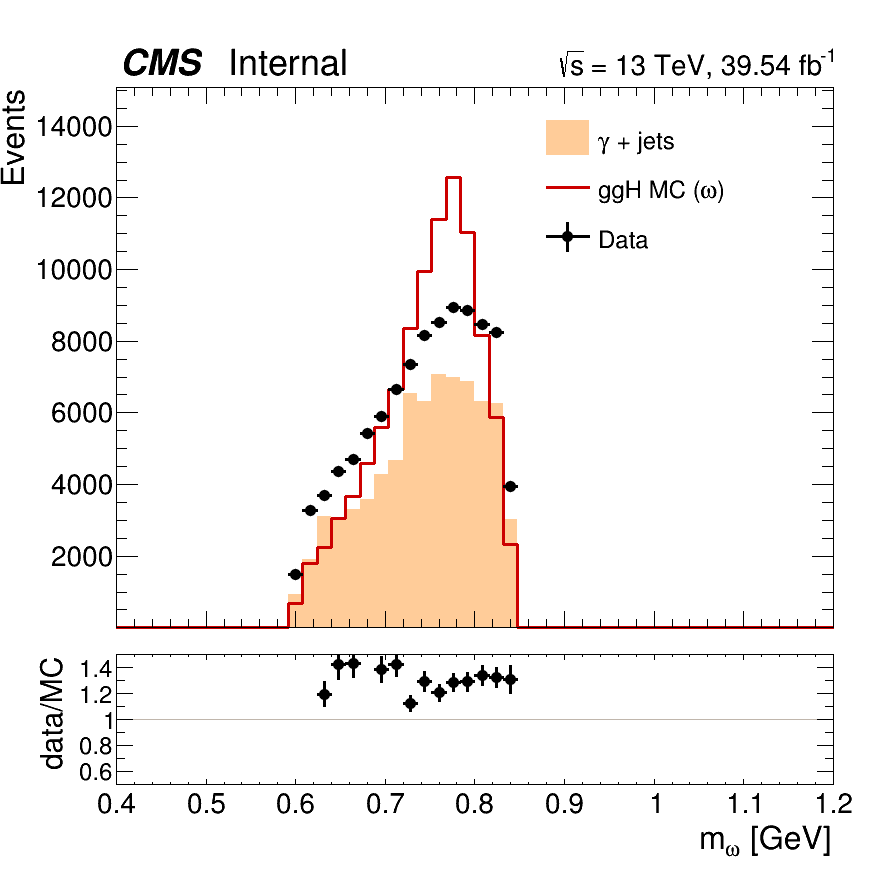
\includegraphics[width=0.49\mylength]{resources/plots/Omega_mass.png}
        \vspace*{-0.2cm}
        \caption{\footnotesize (b)}
    \end{subfigure}%\begin{subfigure}[t]{0.50\mylength}\baselineskip
    \vskip\baselineskip
    \vspace*{-0.5cm}
    \begin{subfigure}[t]{0.50\mylength}
        \centering
        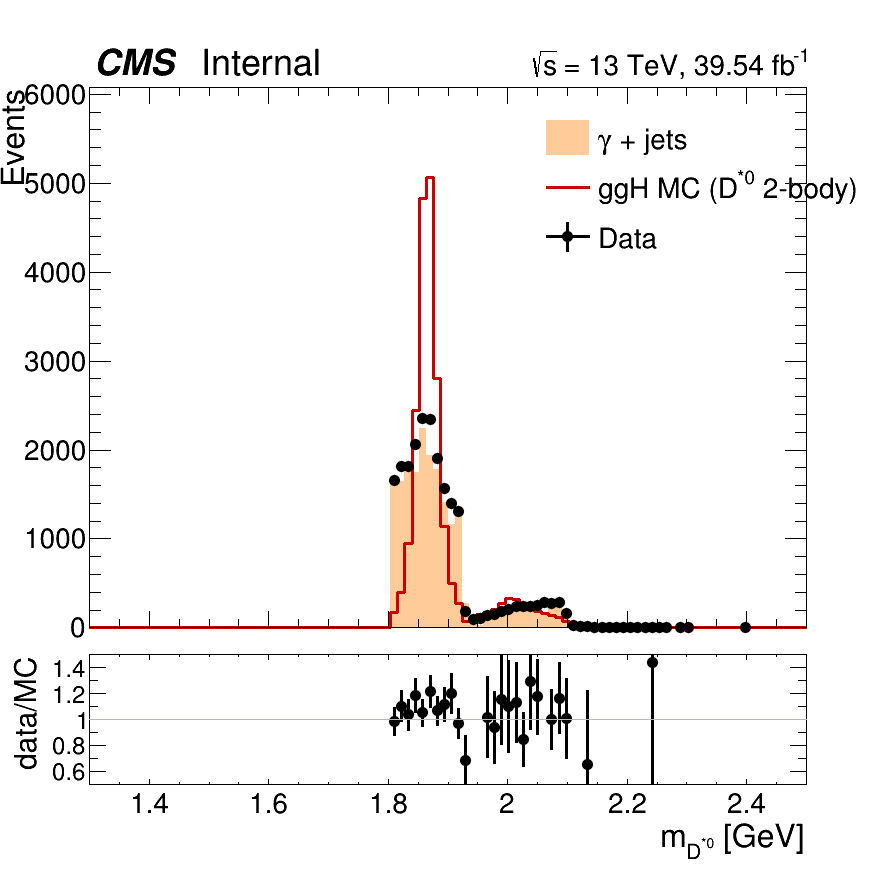
\includegraphics[width=0.49\mylength]{resources/plots/D0Star_2body_mass.png}
        \vspace*{-0.2cm}
        \caption{\footnotesize (c)}
    \end{subfigure}%
    \begin{subfigure}[t]{0.50\mylength}
        \centering
        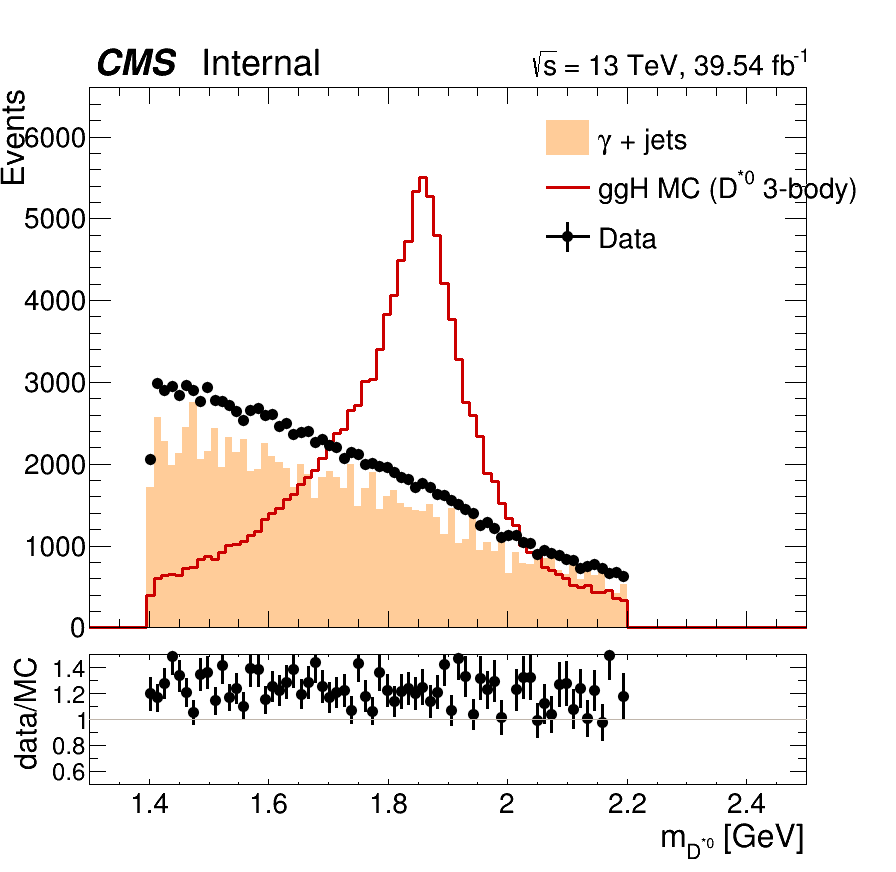
\includegraphics[width=0.49\mylength]{resources/plots/D0Star_3body_mass.png}
        \vspace*{-0.2cm}
        \caption{\footnotesize (d)}
    \end{subfigure}%\begin{subfigure}[t]{0.50\mylength}\baselineskip
\caption{Full meson's mass of the different studied decay modes. (a) $\phi$ channel, (b) $\omega$ channel, (c) $\text{D}^{*0}$ 2-body channel, and (d) $\text{D}^{*0}$ 3-body channel. The MC background is shown in orange, scatter points represent real data, and the signal, in red, is normalized to the data for better visualization.}
\label{fig:full_mass_data}
    \vspace*{-0.0cm}
\end{figure}
Figure \ref{fig:full_mass_data} (c) presents two peaks, one around 1.86 GeV, and another much more sublte around 2 GeV. This is because in approximately $\sim 87\%$ of events, no photon compatible with the decay of a neutral particle is recovered, and therefore the computed full mass of the $\text{D}^{*0}$ is the same as the ditrack system's mass. This is why this variable is not used in the BDT for regressing the transverse momentum (see Section \ref{sec:meson_reconstruction}). All other channels full meson mass, shown in Figures \ref{fig:full_mass_data} (a), (b) and (d), consist of one sharp asymmetric peak. This asymmetric left shoulder is a sign of missing energy. It is worth noting that for the $\text{D}^{*0}$ 3-body decay mode, the peak of the full meson's mass is around 1.85 GeV instead of around the theoretical value of the $\text{D}^{*0}$'s mass, which is 2.007 GeV. The reason for this is that in most of the events, the recovered photons are from the decay of the more energetic $\pi^0$ of the decay $\text{D}^{0}\decaysto \text{K}^{-}\pi^{+}\pi^0$. Therefore, the full meson reconstructed mass resembles more the $\text{D}^{0}$'s mass rather than the $\text{D}^{*0}$'s mass. These singular peaks, that differ from the shape of the background, will also be exploited when modelling the signal, as done for the $\text{D}^{*0}$ 2-body decay mode with its ditrack mass. Additionally, the MC background is consistent with the data across all decay modes.

It is worth noting that the background and data also show subtle peaks in the same position as the signal for certain mass variables, as seen in Figure \ref{fig:ditrack_mass_data} (c) and Figure \ref{fig:full_mass_data} (a) and (b). These peaks arise from real mesons present in the background, unrelated to the signal under study. In future analysis iterations, they could be accounted for by making the background model more complex, as explained in Section \ref{sec:future_improvements}.

\newpage

Figure \ref{fig:photon_pt_data} presents the transverse momentum of the primary photon originating directly from the Higgs boson decay. The signal peaks at around 60 GeV for all channels, which is roughly half of the Higgs boson's mass. This is consistent with Figure \ref{fig:full_pt_data}, which shows the transverse momentum of each meson. In every channel, the signal also peaks around 60 GeV, which with the transverse momentum of the photon adds up to the 125 GeV of the Higgs boson's mass. In these two figures, the MC background is compatible with the data across all decay modes.
\begin{figure}[!ht]
    \captionsetup[subfigure]{labelformat=empty}
    \vspace*{-0.2cm}
    \centering
    \setlength{\mylength}{\textwidth}
    \begin{subfigure}[t]{0.50\mylength}
        \centering
        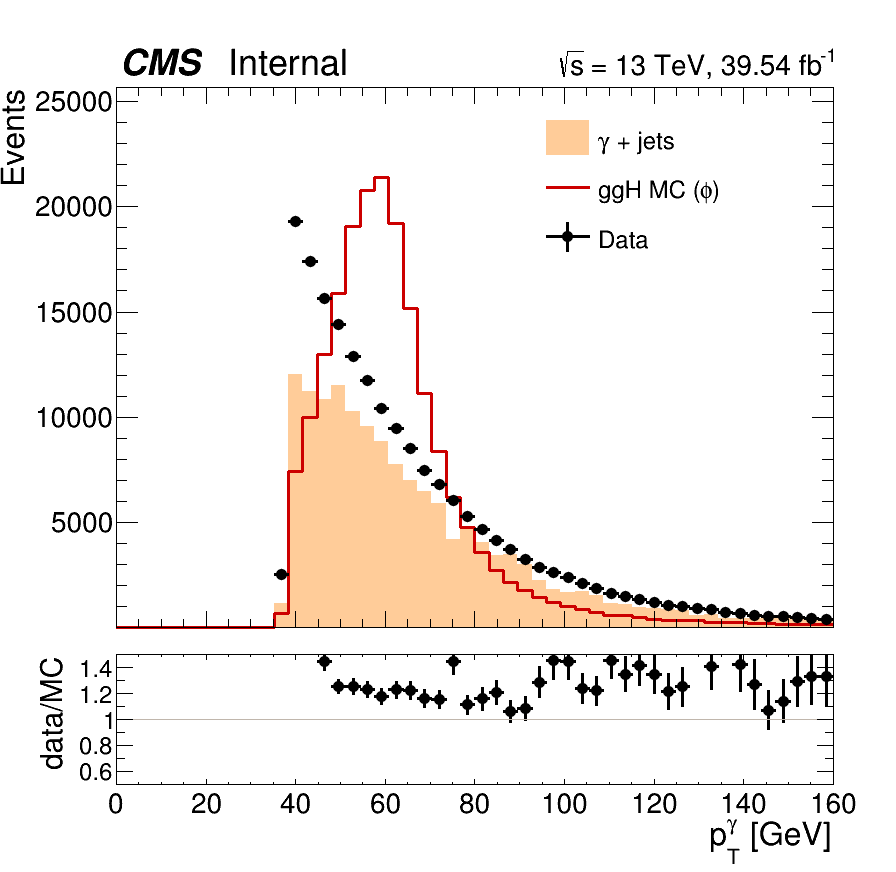
\includegraphics[width=0.49\mylength]{resources/plots/Phi3_photon_pt.png}
        \vspace*{-0.2cm}
        \caption{\footnotesize (a)}
    \end{subfigure}%
    \begin{subfigure}[t]{0.50\mylength}
        \centering
        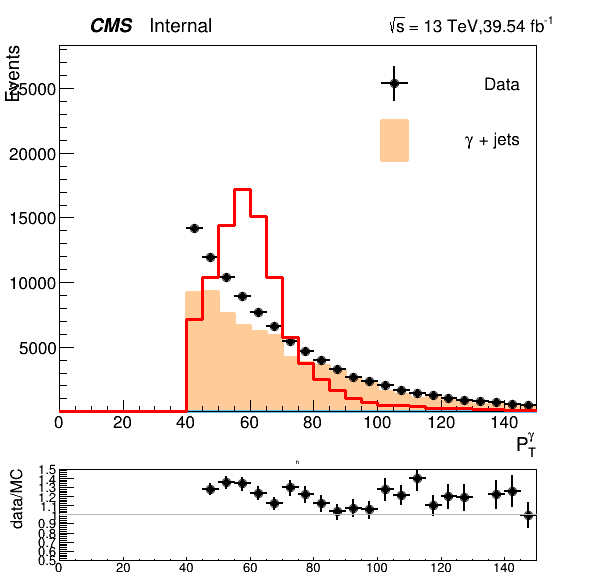
\includegraphics[width=0.49\mylength]{resources/plots/Omega_photon_pt.png}
        \vspace*{-0.2cm}
        \caption{\footnotesize (b)}
    \end{subfigure}%\begin{subfigure}[t]{0.50\mylength}\baselineskip
    \vskip\baselineskip
    \vspace*{-0.5cm}
    \begin{subfigure}[t]{0.50\mylength}
        \centering
        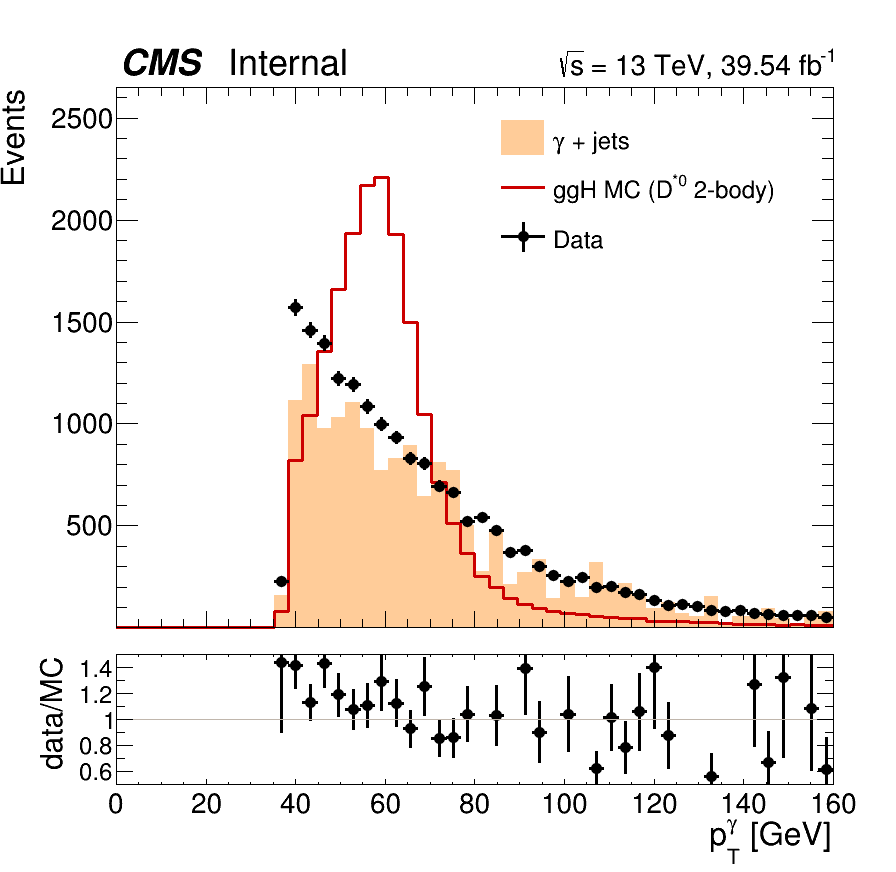
\includegraphics[width=0.49\mylength]{resources/plots/D0Star_2body_photon_pt.png}
        \vspace*{-0.2cm}
        \caption{\footnotesize (c)}
    \end{subfigure}%
    \begin{subfigure}[t]{0.50\mylength}
        \centering
        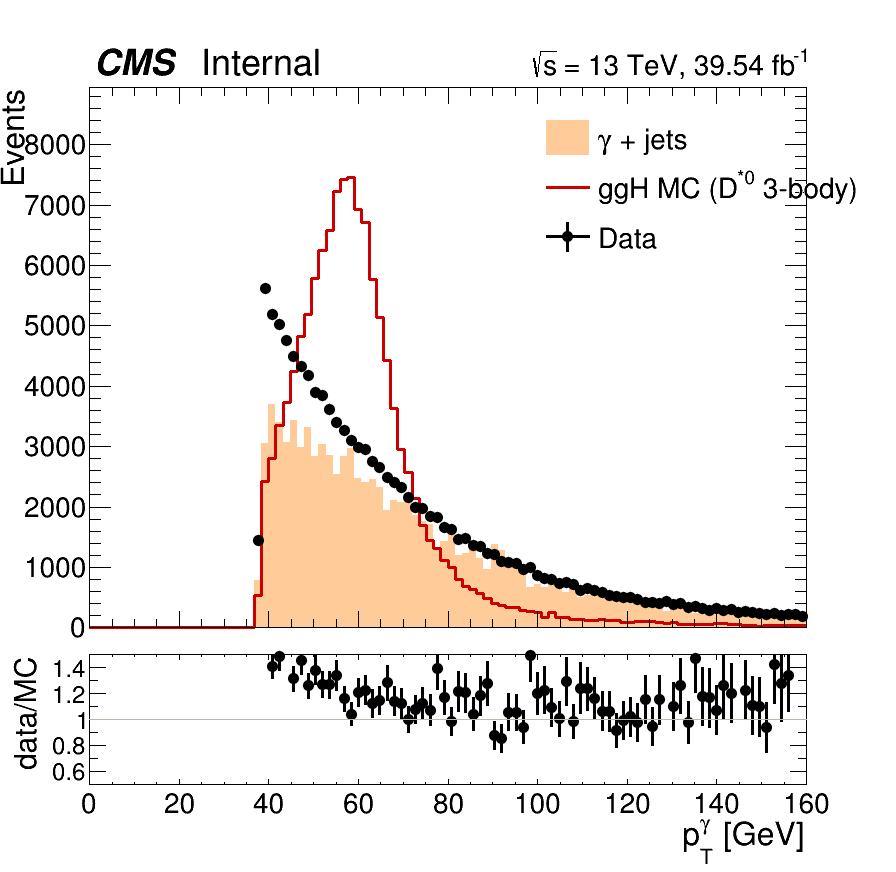
\includegraphics[width=0.49\mylength]{resources/plots/D0Star_3body_photon_pt.png}
        \vspace*{-0.2cm}
        \caption{\footnotesize (d)}
    \end{subfigure}%\begin{subfigure}[t]{0.50\mylength}\baselineskip
\caption{Transverse momentum $\pT$ of the primary photon from the Higgs boson decay, for the different studied decay modes. (a) $\phi$ channel, (b) $\omega$ channel, (c) $\text{D}^{*0}$ 2-body channel, and (d) $\text{D}^{*0}$ 3-body channel. The MC background is shown in orange, scatter points represent real data, and the signal, in red, is normalized to the data for better visualization.}
\label{fig:photon_pt_data}
    \vspace*{-0.0cm}
\end{figure}

\begin{figure}[!ht]
    \captionsetup[subfigure]{labelformat=empty}
    \vspace*{-0.2cm}
    \centering
    \setlength{\mylength}{\textwidth}
    \begin{subfigure}[t]{0.50\mylength}
        \centering
        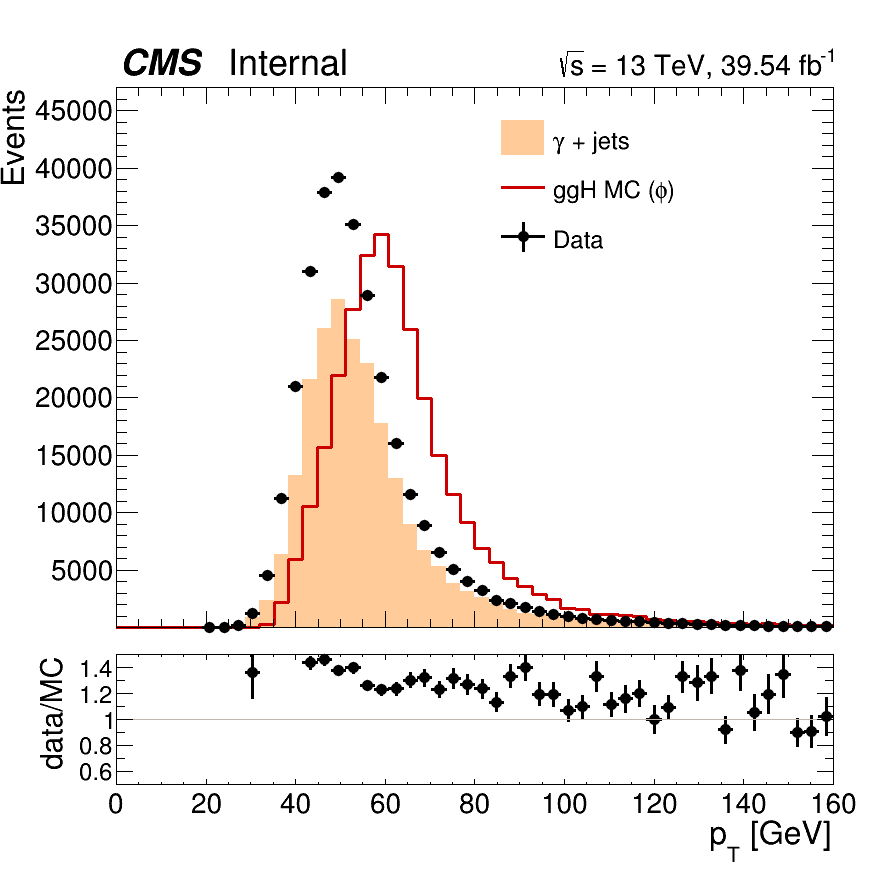
\includegraphics[width=0.49\mylength]{resources/plots/Phi3_pt.png}
        \vspace*{-0.2cm}
        \caption{\footnotesize (a)}
    \end{subfigure}%
    \begin{subfigure}[t]{0.50\mylength}
        \centering
        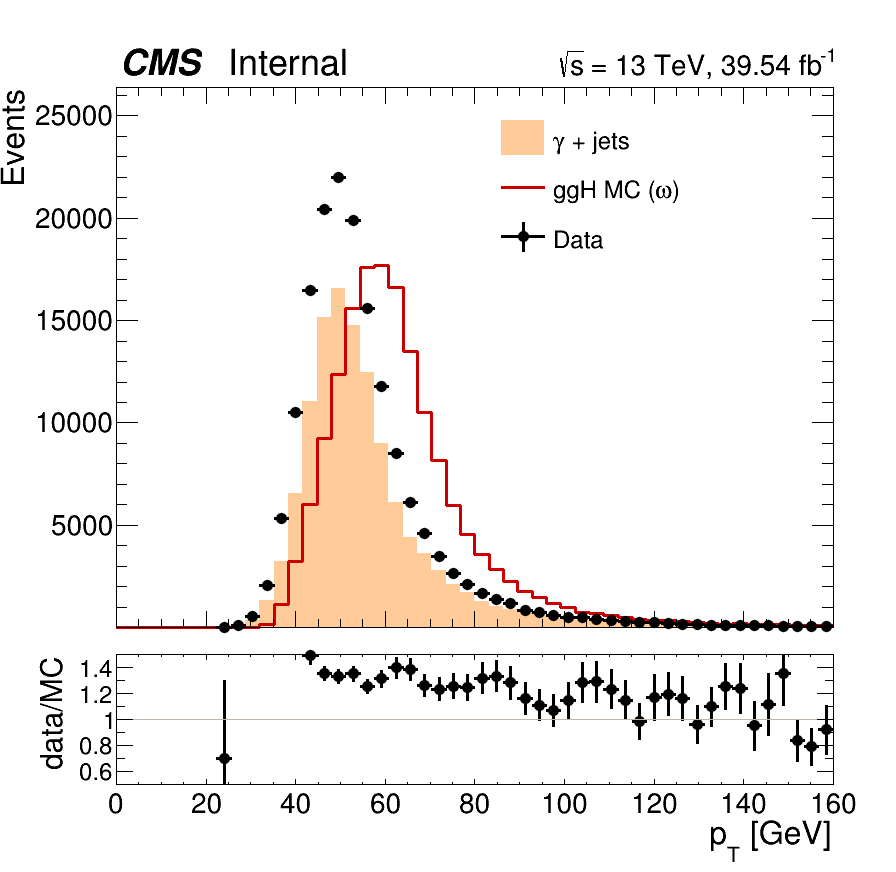
\includegraphics[width=0.49\mylength]{resources/plots/Omega_pt.png}
        \vspace*{-0.2cm}
        \caption{\footnotesize (b)}
    \end{subfigure}%\begin{subfigure}[t]{0.50\mylength}\baselineskip
    \vskip\baselineskip
    \vspace*{-0.5cm}
    \begin{subfigure}[t]{0.50\mylength}
        \centering
        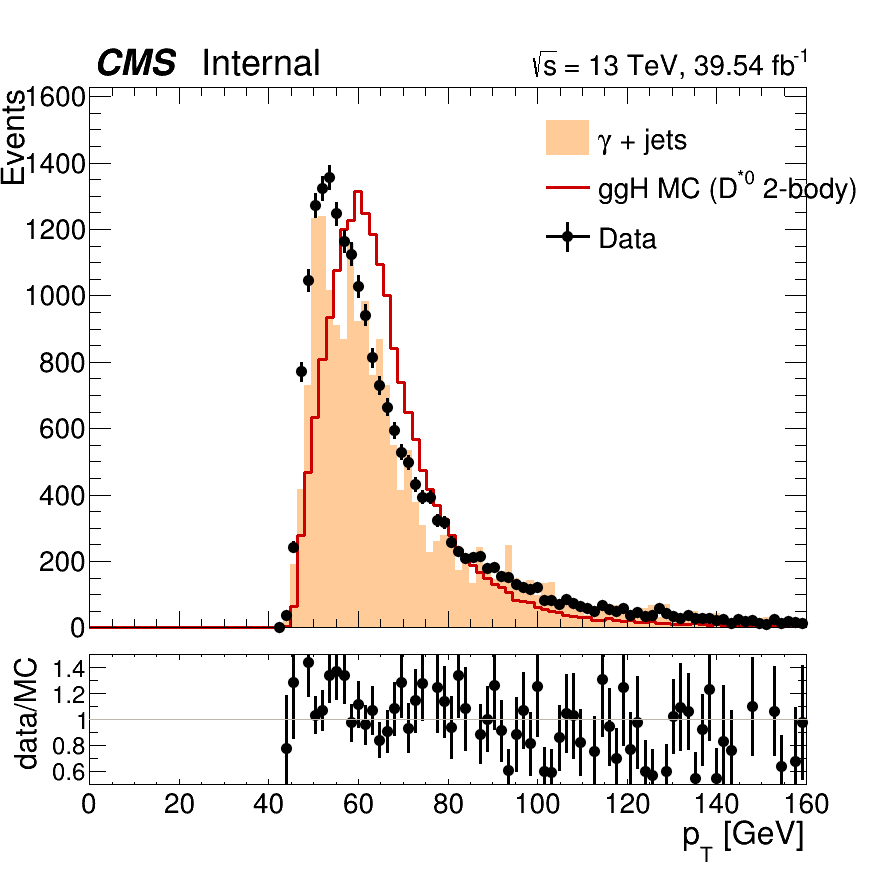
\includegraphics[width=0.49\mylength]{resources/plots/D0Star_2body_pt.png}
        \vspace*{-0.2cm}
        \caption{\footnotesize (c)}
    \end{subfigure}%
    \begin{subfigure}[t]{0.50\mylength}
        \centering
        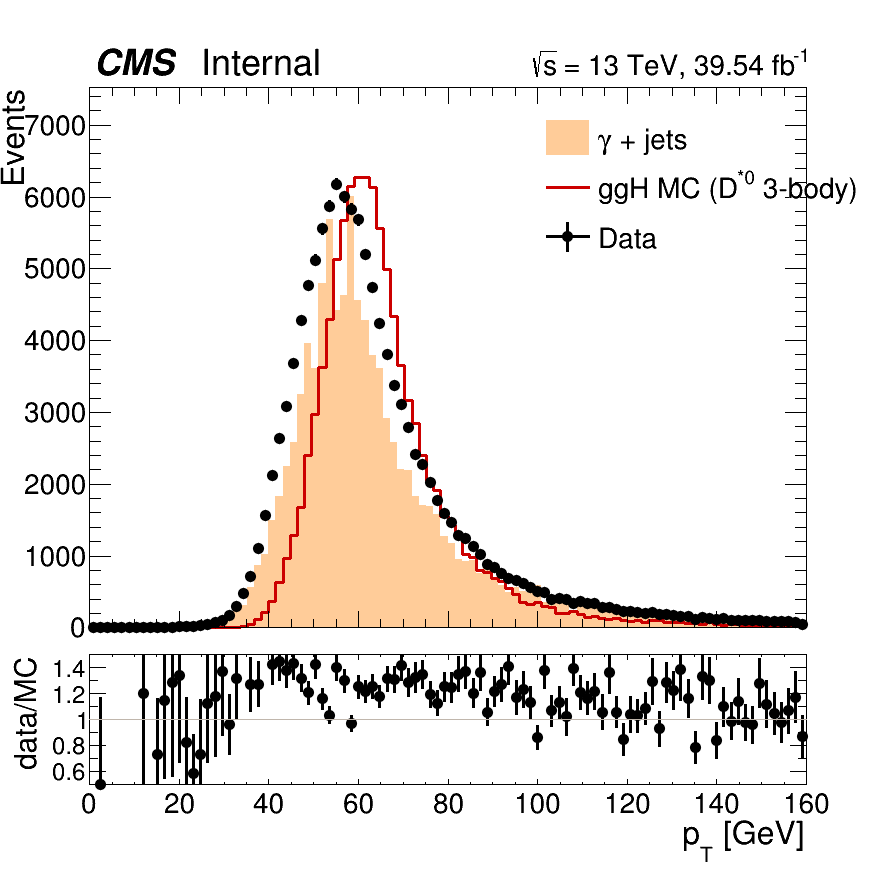
\includegraphics[width=0.49\mylength]{resources/plots/D0Star_3body_pt.png}
        \vspace*{-0.2cm}
        \caption{\footnotesize (d)}
    \end{subfigure}%\begin{subfigure}[t]{0.50\mylength}\baselineskip
\caption{Transverse momentum $\pT$ of the full meson for the different studied decay modes. (a) $\phi$ channel, (b) $\omega$ channel, (c) $\text{D}^{*0}$ 2-body channel, and (d) $\text{D}^{*0}$ 3-body channel. The MC background is shown in orange, scatter points represent real data, and the signal, in red, is normalized to the data for better visualization.}
\label{fig:full_pt_data}
    \vspace*{-0.0cm}
\end{figure}

\newpage

\clearpage

Figures \ref{fig:lead_pt_data} and \ref{fig:sublead_pt_data} illustrate the transverse momentum of the charged leading and subleading tracks for each decay mode. All channels show a similar shape for the signal. However, it is worth noting that in the $\text{D}^{*0}$ 2-body decay, both the leading and subleading tracks are more energetic, as this is the only scenario where $\text{D}^{0}$ decays into just two charged tracks (the neutral particle from $\text{D}^{*0}\decaysto \text{D}^{0}\pi^{0}/\gamma$ typically carries around $\sim5$ GeV in energy). As with all other figures in this section, the data-MC background comparison appears compatible across all decay modes.

\begin{figure}[!ht]
    \captionsetup[subfigure]{labelformat=empty}
    \vspace*{-0.2cm}
    \centering
    \setlength{\mylength}{\textwidth}
    \begin{subfigure}[t]{0.50\mylength}
        \centering
        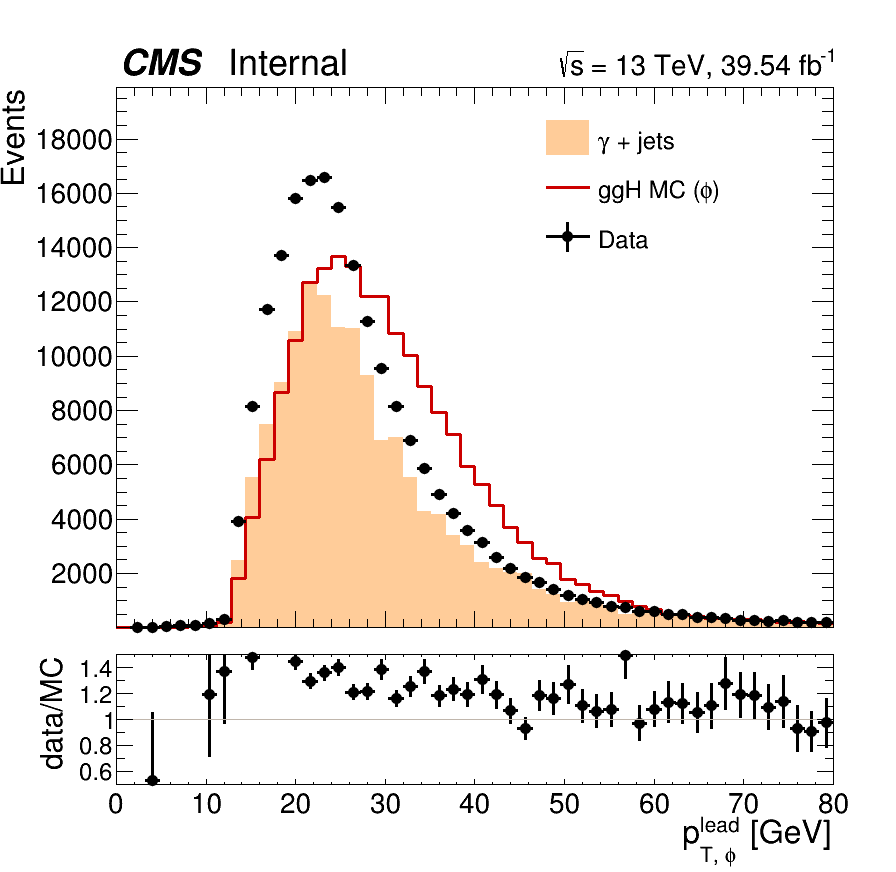
\includegraphics[width=0.49\mylength]{resources/plots/Phi3_lead_pt.png}
        \vspace*{-0.2cm}
        \caption{\footnotesize (a)}
    \end{subfigure}%
    \begin{subfigure}[t]{0.50\mylength}
        \centering
        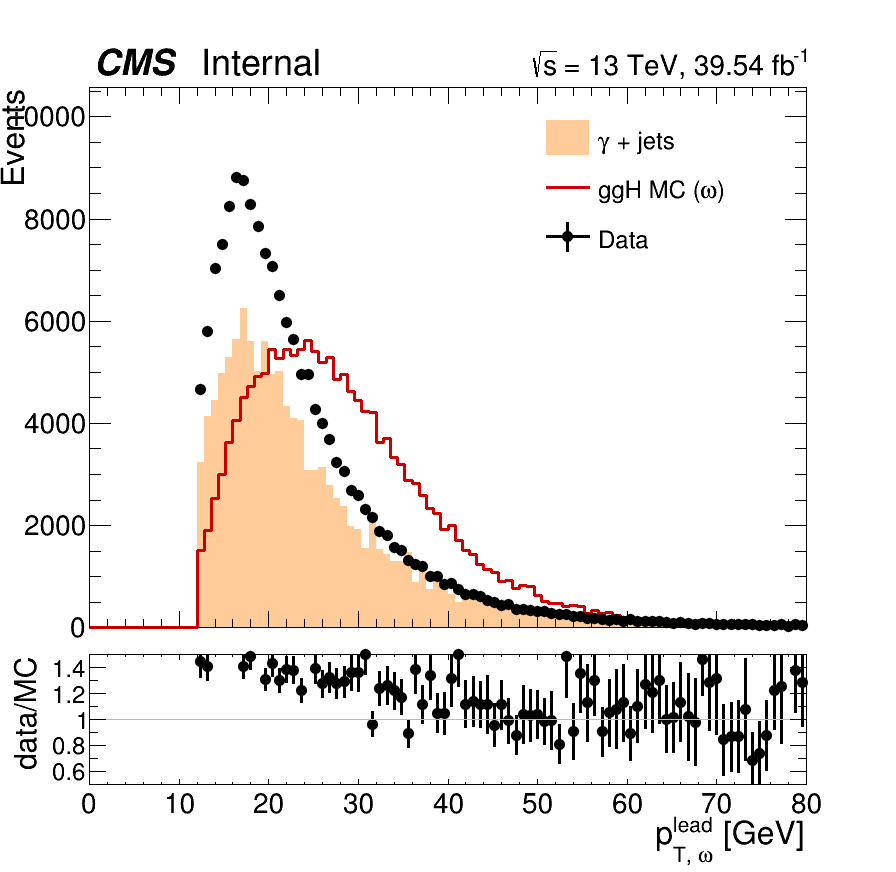
\includegraphics[width=0.49\mylength]{resources/plots/Omega_lead_pt.png}
        \vspace*{-0.2cm}
        \caption{\footnotesize (b)}
    \end{subfigure}%\begin{subfigure}[t]{0.50\mylength}\baselineskip
    \vskip\baselineskip
    \vspace*{-0.5cm}
    \begin{subfigure}[t]{0.50\mylength}
        \centering
        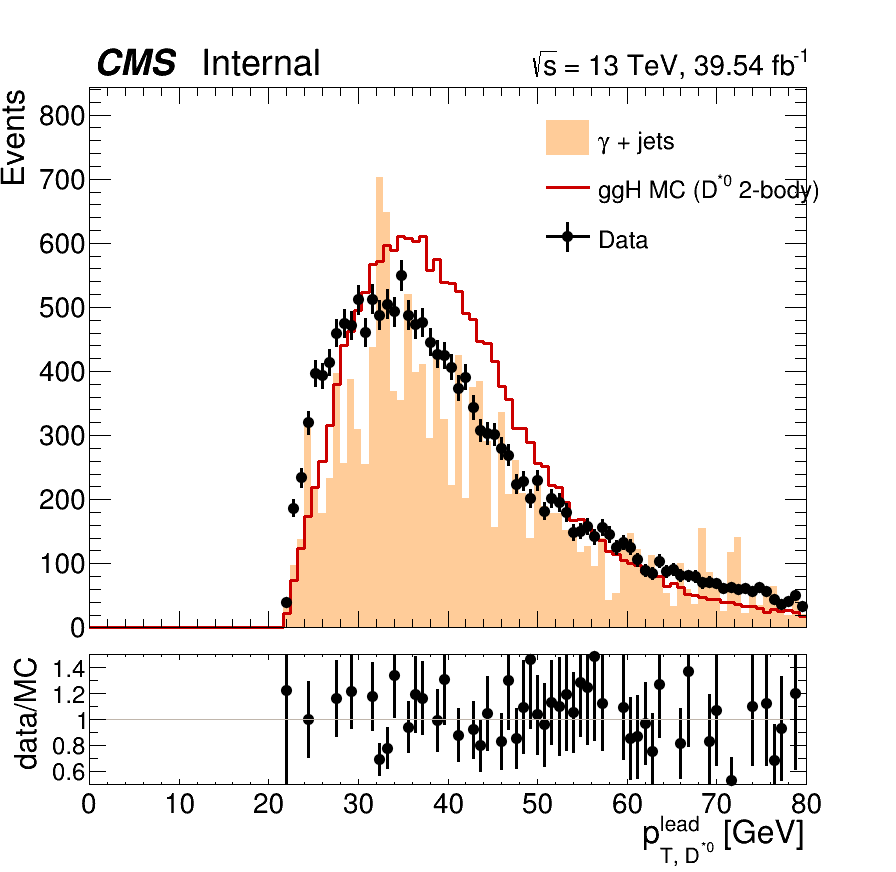
\includegraphics[width=0.49\mylength]{resources/plots/D0Star_2body_lead_pt.png}
        \vspace*{-0.2cm}
        \caption{\footnotesize (c)}
    \end{subfigure}%
    \begin{subfigure}[t]{0.50\mylength}
        \centering
        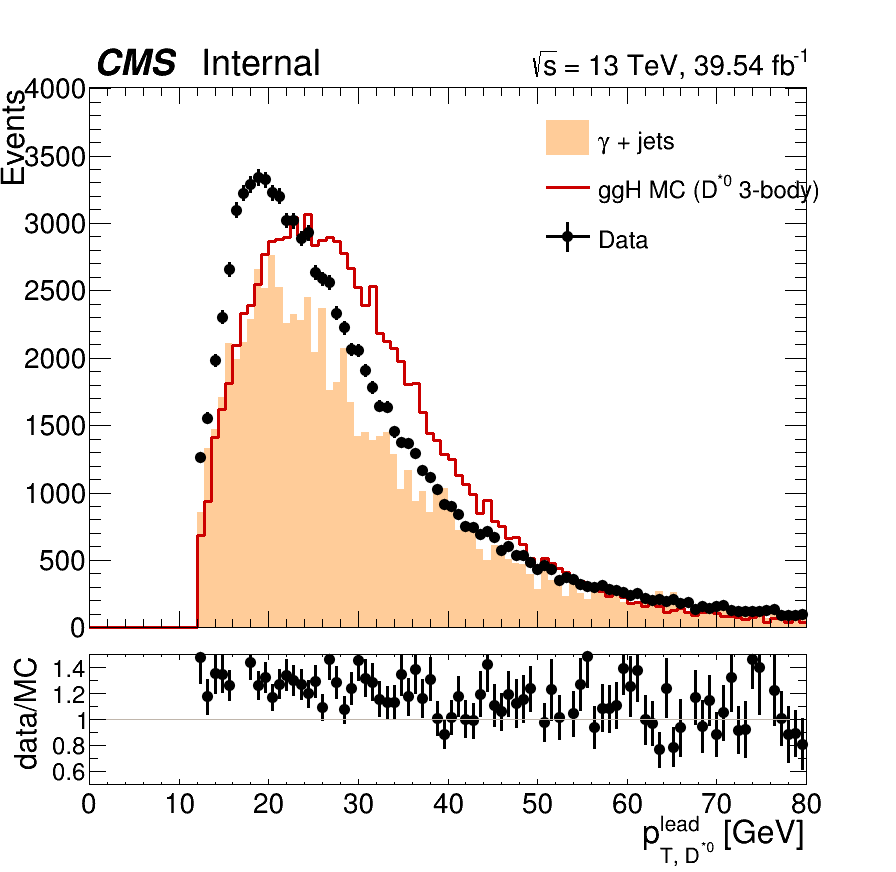
\includegraphics[width=0.49\mylength]{resources/plots/D0Star_3body_lead_pt.png}
        \vspace*{-0.2cm}
        \caption{\footnotesize (d)}
    \end{subfigure}%\begin{subfigure}[t]{0.50\mylength}\baselineskip
\caption{Transverse momentum $\pT$ of the leading charged track for the different studied decay modes. (a) $\phi$ channel, (b) $\omega$ channel, (c) $\text{D}^{*0}$ 2-body channel, and (d) $\text{D}^{*0}$ 3-body channel. The MC background is shown in orange, scatter points represent real data, and the signal, in red, is normalized to the data for better visualization.}
\label{fig:lead_pt_data}
    \vspace*{-0.0cm}
\end{figure}

\begin{figure}[!ht]
    \captionsetup[subfigure]{labelformat=empty}
    \vspace*{-0.2cm}
    \centering
    \setlength{\mylength}{\textwidth}
    \begin{subfigure}[t]{0.50\mylength}
        \centering
        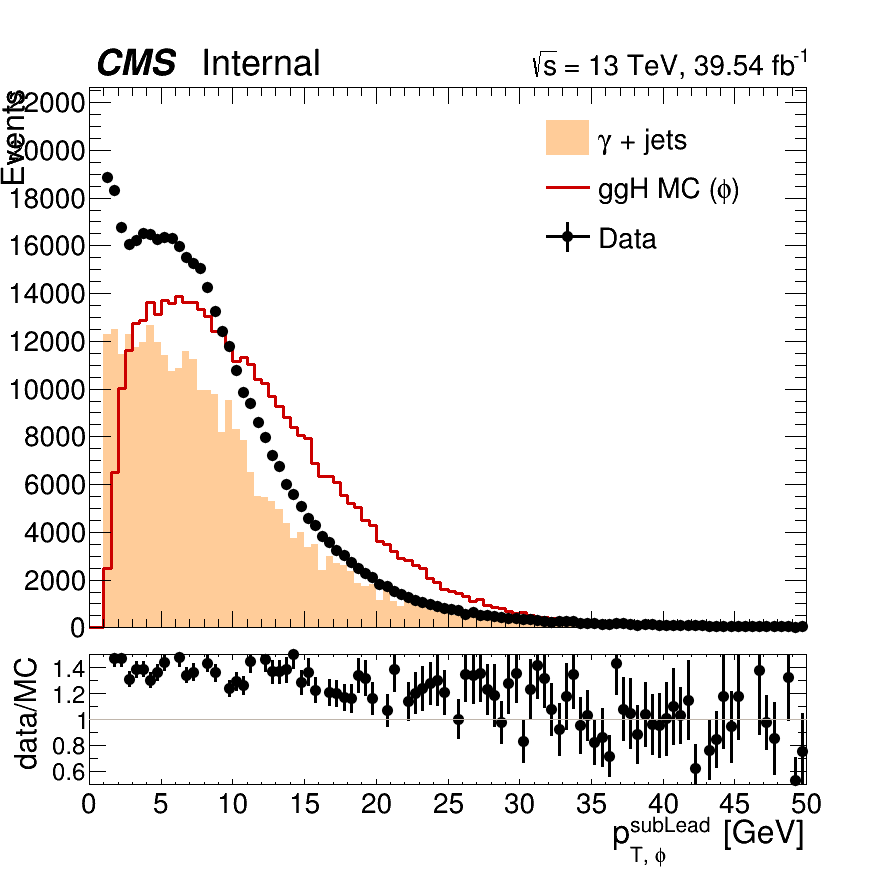
\includegraphics[width=0.49\mylength]{resources/plots/Phi3_sublead_pt.png}
        \vspace*{-0.2cm}
        \caption{\footnotesize (a)}
    \end{subfigure}%
    \begin{subfigure}[t]{0.50\mylength}
        \centering
        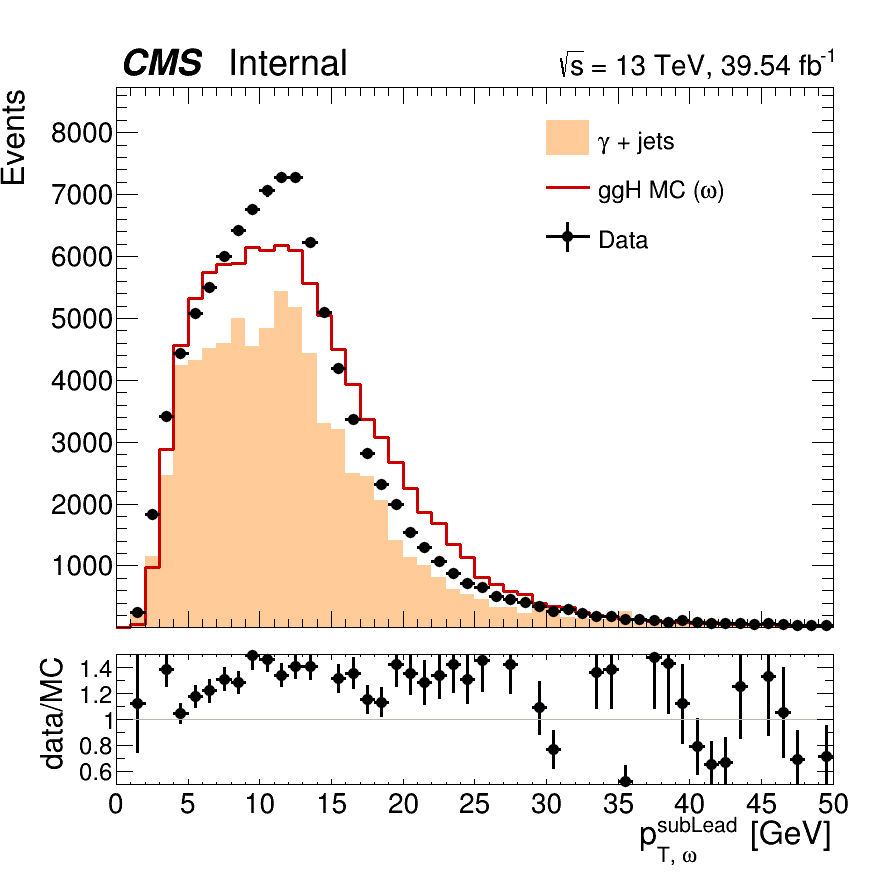
\includegraphics[width=0.49\mylength]{resources/plots/Omega_sublead_pt.png}
        \vspace*{-0.2cm}
        \caption{\footnotesize (b)}
    \end{subfigure}%\begin{subfigure}[t]{0.50\mylength}\baselineskip
    \vskip\baselineskip
    \vspace*{-0.5cm}
    \begin{subfigure}[t]{0.50\mylength}
        \centering
        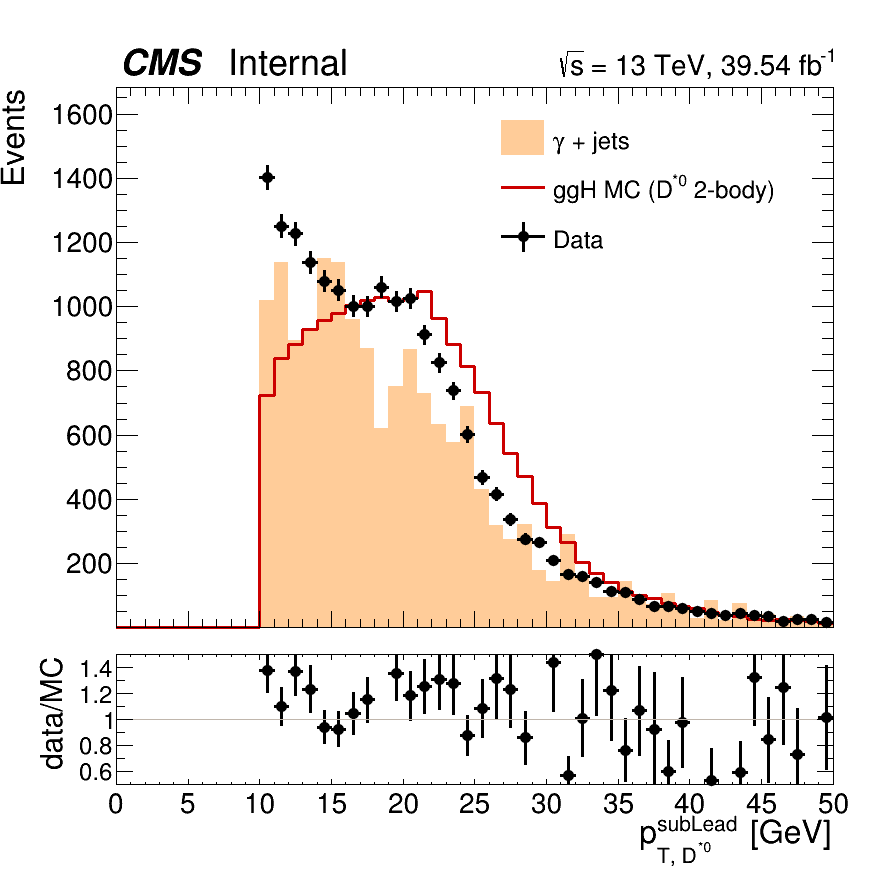
\includegraphics[width=0.49\mylength]{resources/plots/D0Star_2body_sublead_pt.png}
        \vspace*{-0.2cm}
        \caption{\footnotesize (c)}
    \end{subfigure}%
    \begin{subfigure}[t]{0.50\mylength}
        \centering
        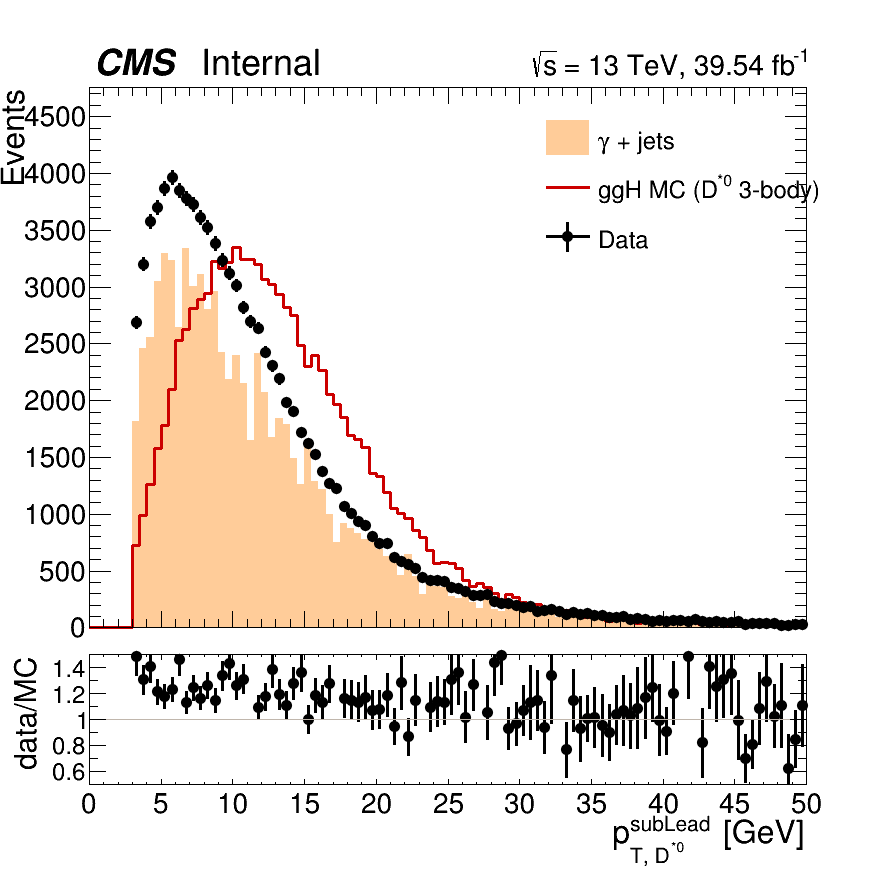
\includegraphics[width=0.49\mylength]{resources/plots/D0Star_3body_sublead_pt.png}
        \vspace*{-0.2cm}
        \caption{\footnotesize (d)}
    \end{subfigure}%\begin{subfigure}[t]{0.50\mylength}\baselineskip
\caption{Transverse momentum $\pT$ of the subleading charged track for the different studied decay modes. (a) $\phi$ channel, (b) $\omega$ channel, (c) $\text{D}^{*0}$ 2-body channel, and (d) $\text{D}^{*0}$ 3-body channel. The MC background is shown in orange, scatter points represent real data, and the signal, in red, is normalized to the data for better visualization.}
\label{fig:sublead_pt_data}
    \vspace*{-0.0cm}
\end{figure}

\clearpage

\section{Signal and background modelling}\label{sec:modelling}

The first approach to extract the potential Higgs boson signal is done by fitting the invariant mass distribution $m^{\text{H}}_{\gamma, M}$ for each decay mode separately, since the signal is expected to show a peak over a monotonous background. Both the signal and background are directly estimated from MC (signal) or data (background) by fitting the photon-meson invariant mass spectrum with analytical functions in the region $100 < m^{\text{H}}_{\gamma, M} < 160$ GeV. The RooFit framework \cite{CERN:root_roofit}, a toolkit provided within the \verb+ROOT+ module for modelling the expected event distribution, is used for this purpose, and a binned maximum likelihood fit is conducted.

\begin{figure}[!ht]
    \captionsetup[subfigure]{labelformat=empty}
    \vspace*{-0.2cm}
    \centering
    \setlength{\mylength}{\textwidth}
    \begin{subfigure}[t]{0.50\mylength}
        \centering
        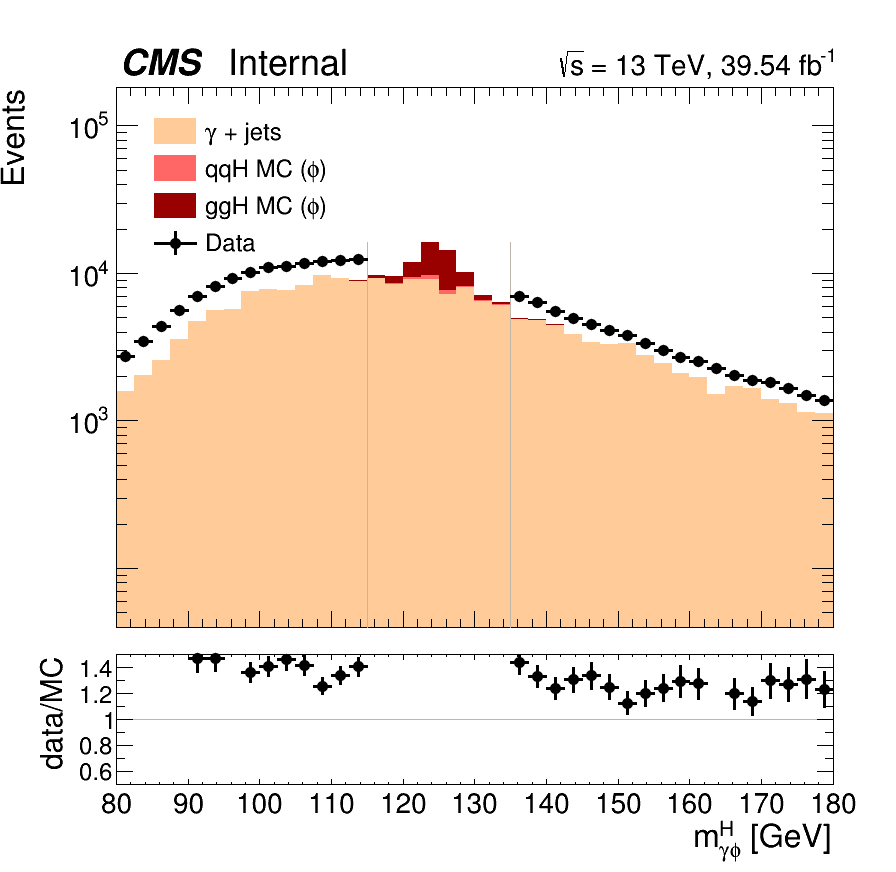
\includegraphics[width=0.49\mylength]{resources/plots/Phi3_HiggsMass.png}
        \vspace*{-0.2cm}
        \caption{\footnotesize (a)}
    \end{subfigure}%
    \begin{subfigure}[t]{0.50\mylength}
        \centering
        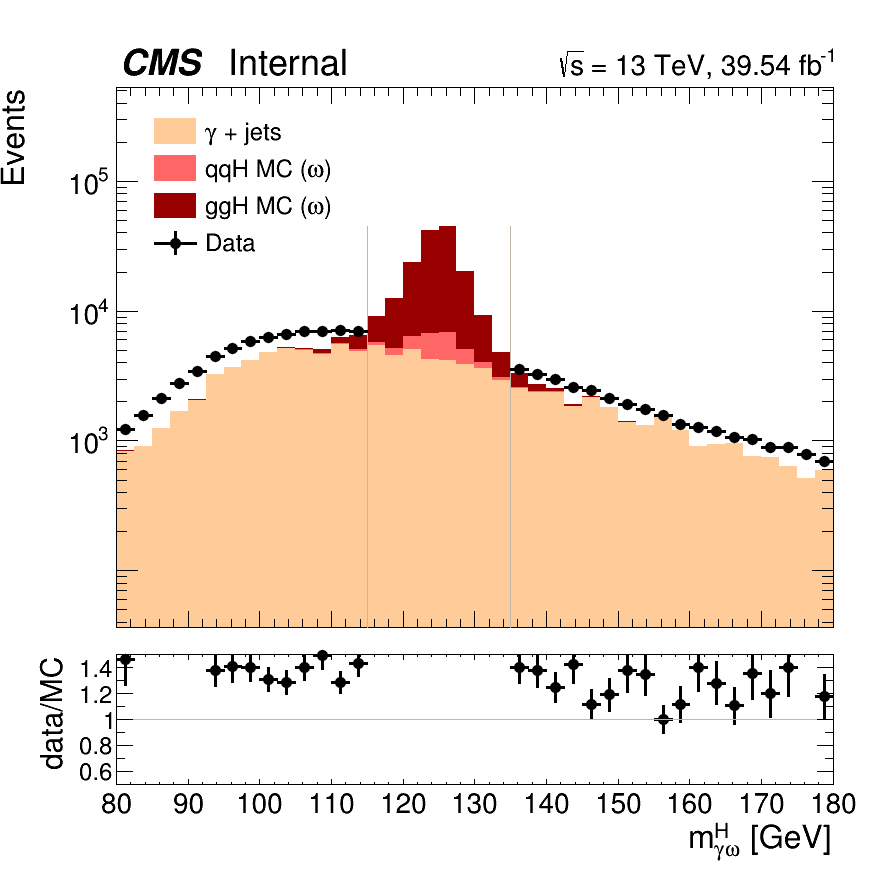
\includegraphics[width=0.49\mylength]{resources/plots/Omega_HiggsMass.png}
        \vspace*{-0.2cm}
        \caption{\footnotesize (b)}
    \end{subfigure}%\begin{subfigure}[t]{0.50\mylength}\baselineski
    \vskip\baselineskip
    \vspace*{-0.5cm}
    \begin{subfigure}[t]{0.50\mylength}
        \centering
        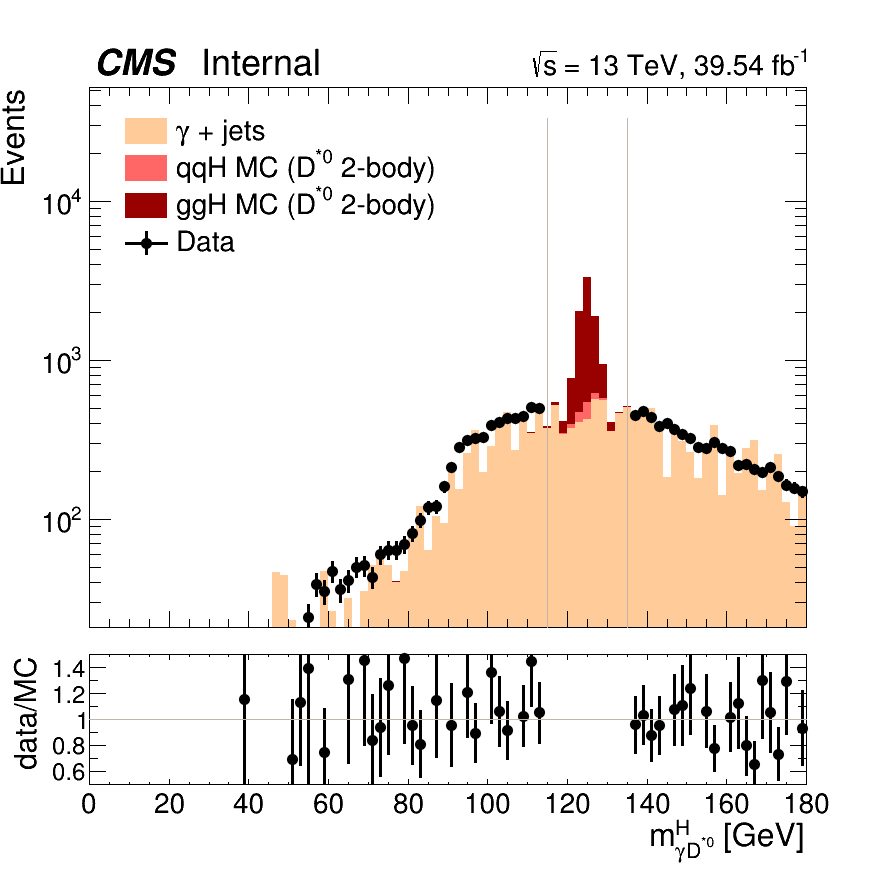
\includegraphics[width=0.49\mylength]{resources/plots/D0Star_2body_HiggsMass.png}
        \vspace*{-0.2cm}
        \caption{\footnotesize (c)}
    \end{subfigure}%
    \begin{subfigure}[t]{0.50\mylength}
        \centering
        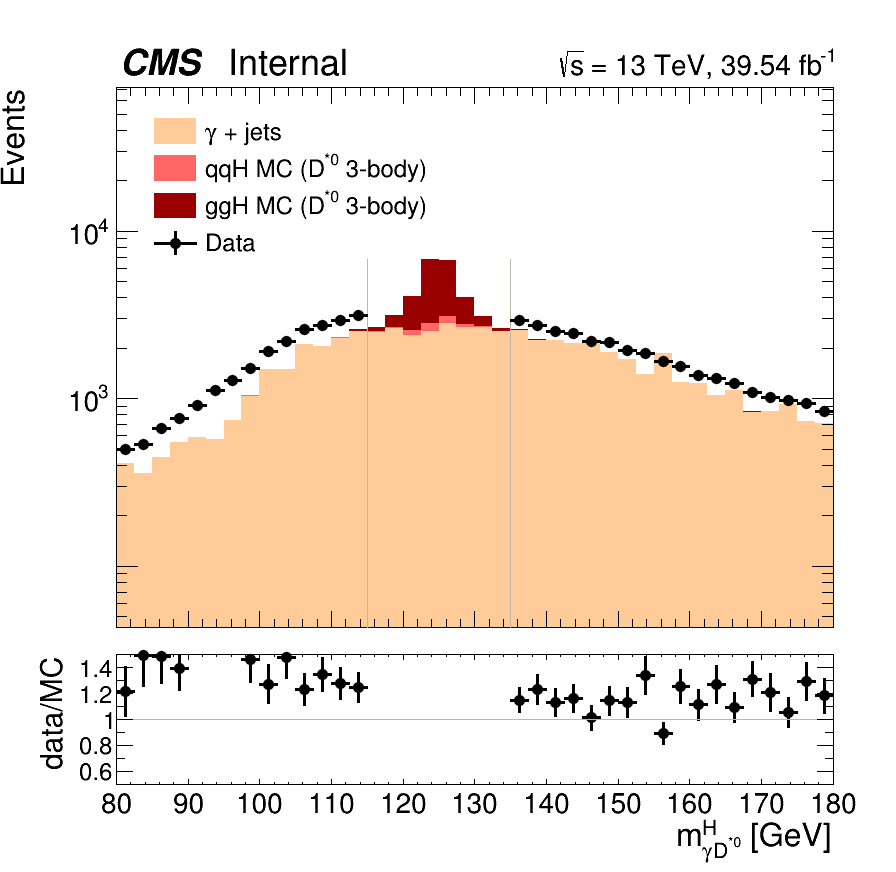
\includegraphics[width=0.49\mylength]{resources/plots/D0Star_3body_HiggsMass.png}
        \vspace*{-0.2cm}
        \caption{\footnotesize (d)}
    \end{subfigure}%\begin{subfigure}[t]{0.50\mylength}\baselineskip
\caption{Higgs invariant mass distribution $m^{\text{H}}_{\gamma, M}$ for the different studied decay modes. (a) $\phi$ channel, (b) $\omega$ channel, (c) $\text{D}^{*0}$ 2-body channel, and (d) $\text{D}^{*0}$ 3-body channel. The MC $\gamma$ + jets background is shown in orange, scatter points represent real data, the ggH MC signal in crimson and the qqH MC signal in light coral. The total MC signal is scaled so that $\mathcal{B}(\text{H}\protect\decaysto \phi\gamma)$, $\mathcal{B}(\text{H}\protect\decaysto \omega\gamma)$ or $\mathcal{B}(\text{H}\protect\decaysto \text{D}^{*0}\gamma)$ is set to 1 for better visualization. The data is blinded in the region of interest.}
\label{fig:Higgs_mass_data}
    \vspace*{-0.0cm}
\end{figure}
Figure \ref{fig:Higgs_mass_data} displays the photon-meson invariant mass distribution $m^{\text{H}}_{\gamma, M}$ for each channel. The data in the region of interest is not shown, it is still \textit{blinded}. Only after completing the full analysis and ensuring the consistency of the techniques used can the data be unblinded to enable actual measurements. This approach is commonly employed in high-energy physics to maintain an unbiased study.

Based on the earlier discussed selection criteria, the shape of the data and background exhibit a turn-on structure in $m^{\text{H}}_{\gamma, M}$. This turn-on varies for each decay mode due to the kinematic constraints of the events and the imposed selection cuts.

As shown in Figure \ref{fig:Higgs_mass_data}, for all decay modes, the signal presents a sharp peak around the mass of the Higgs boson, $m_{\text{H}}=125$ GeV, while the background is either flat or monotonically decreasing. The primary contribution comes from ggH, but VBF (also denoted as qqH) shows a non-negligible contribution. By not focusing on a single production mode, events from both ggH and VBF are reconstructed, enhancing the signal-to-background ratio.

After performing this one-dimensional fit to $m^{\text{H}}_{\gamma, M}$, a two-dimensional fit has been considered. This 2D model simultaneously fits both the photon-meson invariant mass $m^{\text{H}}_{\gamma, M}$ and the full meson mass $m_{M}$. In the case of the $\text{D}^{*0}$ 2-body decay mode, the ditrack mass $m^{\text{diTrk}}_{M}$ is used instead of the full meson mass, due to the incomplete recovery of the latter. This strategy is the one ultimately adopted.

\subsection{Signal modelling}\label{subsec:sgn_modelling}

Although previously discussed, it is worth emphasizing that the analysis sensitivity relies on the resolution of the photon-meson mass $m^{\text{H}}_{\gamma, M}$, which strongly depends on the kinematics, especially the transverse momentum of the photon and meson.

The first natural iteration of the two-dimensional fit is to consider the two variables as uncorrelated and independent. Under this assumption, the two-dimensional PDF becomes the product of two one-dimensional PDFs. Figure \ref{fig:sig_modelling_sliced} shows the Higgs boson invariant mass for four different intervals of the meson mass for each decay mode.
\begin{figure}[!ht]
    \captionsetup[subfigure]{labelformat=empty}
    \vspace*{-0.2cm}
    \centering
    \setlength{\mylength}{\textwidth}
    \begin{subfigure}[t]{0.50\mylength}
        \centering
        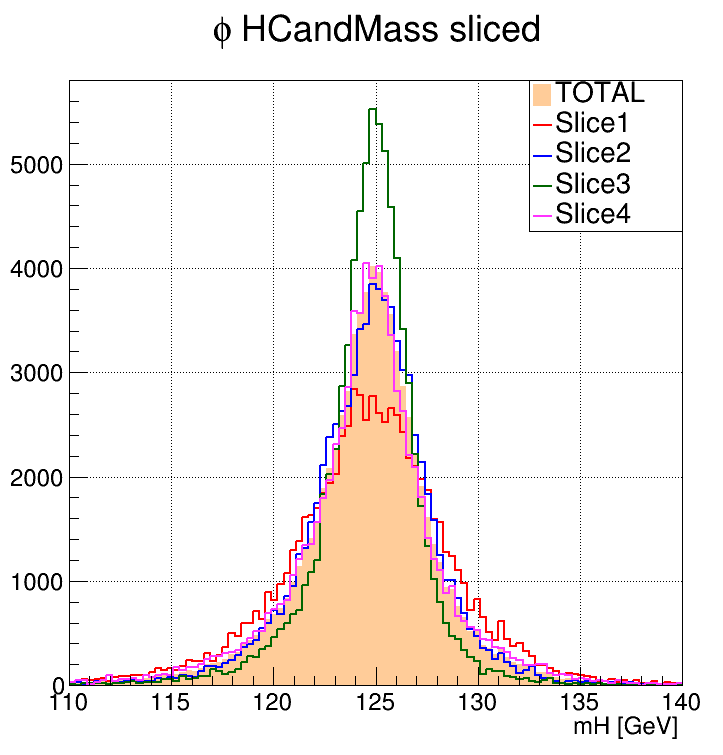
\includegraphics[width=0.49\mylength]{resources/plots/Phi3_fit_SGN_MH_sliced.png}
        \vspace*{-0.2cm}
        \caption{\footnotesize (a)}
    \end{subfigure}%
    \begin{subfigure}[t]{0.50\mylength}
        \centering
        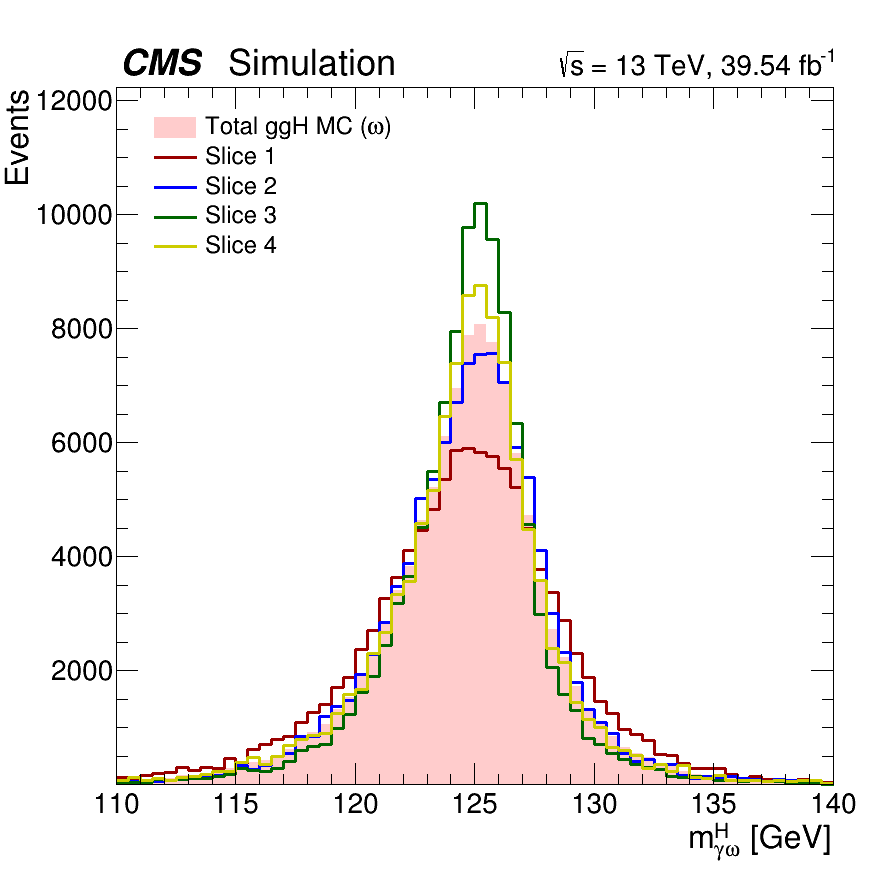
\includegraphics[width=0.49\mylength]{resources/plots/Omega_fit_SGN_MH_sliced.png}
        \vspace*{-0.2cm}
        \caption{\footnotesize (b)}
    \end{subfigure}%\begin{subfigure}[t]{0.50\mylength}\baselineskip
    \vskip\baselineskip
    \vspace*{-0.5cm}
    \begin{subfigure}[t]{0.50\mylength}
        \centering
        \includegraphics[width=0.49\mylength]{resources/plots/D0Star_2body_fit_SGN_MH_sliced.png}
        \vspace*{-0.2cm}
        \caption{\footnotesize (c)}
    \end{subfigure}%
    \begin{subfigure}[t]{0.50\mylength}
        \centering
        \includegraphics[width=0.49\mylength]{resources/plots/D0Star_3body_fit_SGN_MH_sliced.png}
        \vspace*{-0.2cm}
        \caption{\footnotesize (d)}
    \end{subfigure}%\begin{subfigure}[t]{0.50\mylength}\baselineskip
\caption{MC signal photon-meson invariant mass $m^{\text{H}}_{\gamma, M}$ for each decay channel, sliced for different meson mass intervals. (a) $\phi$ channel, (b) $\omega$ channel, (c) $\text{D}^{*0}$ 2-body channel, and (d) $\text{D}^{*0}$ 3-body channel.  The values for the selected slices are displayed in Table \ref{tab:slice_values}. The total photon-meson invariant mass is displayed in light red.}
\label{fig:sig_modelling_sliced}
    \vspace*{-0.0cm}
\end{figure}
Each slice includes events where the recovered meson mass is within a certain interval, normalized to the same area. The values for the selected slices shown in Figure \ref{fig:sig_modelling_sliced} are displayed in Table \ref{tab:slice_values}. In light red, the total photon-meson invariant mass is displayed. It can be observed that this approximation is reasonably good, particularly for the $\text{D}^{*0}$ 2-decay mode, given its precise mass reconstruction. For each channel, every slice has the same shape and the same maximum position, with only slight differences in width. To address this, in further iterations, one should either consider this as an uncertainty of the used model or account for this variation by modifying the 2D function, possibly by adding a correction factor. The 2D-PDF is then fitted to the MC signal, instead of doing two one-dimensional fits.
\begin{table}[!ht]
    \centering
    \begin{tabular}{|l|c|c|c|c|}
        \hline
        \cellcolor{lightgray}Decay channel &\cellcolor{lightgray}Slice 1 (MeV)&\cellcolor{lightgray}Slice 2 (MeV)&\cellcolor{lightgray}Slice 3 (MeV)&\cellcolor{lightgray}Slice 4 (MeV)\\ \hline
        $\phi$                  &$[800, 920]$&$[920, 990]$&$[990, 1030]$&$[1030, 1150]$  \\
        $\omega$                &$[600, 720]$&$[720, 760]$&$[760, 800]$&$[800, 900]$  \\
        $\text{D}^{*0}$ 2-body  &$[1805, 1854]$&$[1854, 1865]$&$[1865, 1876]$&$[1876, 1925]$  \\
        $\text{D}^{*0}$ 3-body  &$[1500, 1710]$&$[1710, 1800]$&$[1800, 1870]$&$[1870, 2100]$  \\
        \hline
        \end{tabular}
    \caption{Intervals selected to slice the mass of the meson, used in Figures \ref{fig:sig_modelling_sliced} and \ref{fig:bkg_modelling_sliced}.}
    \label{tab:slice_values}
\end{table}

The expected photon-meson mass candidate distribution in signal events, for each decay mode, is modelled using a double-sided Crystal Ball. This function, named after the Crystal Ball Collaboration \cite{A2:CB}, is a probability density function (PDF) commonly employed in high-energy physics (HEP). It consists of a Gaussian centre and two asymmetric tails modelled by power-law functions, and it is $\mathcal{C}^{1}$, i.e., continuous with a continuous derivative. This functional form simultaneously offers a robust description of the Higgs boson mass spectrum and a straightforward way to incorporate shape uncertainties, as it has only one parameter associated with the peak and two with the width of the lineshape. The tails are necessary to account for the non-Gaussian response of the photons and meson. Further information about this PDF and its implementation in \verb+ROOT+ is available in Ref. \cite{CERN:root_CB}. The full (ditrack) meson's mass is also modelled with a double-sided Crystal Ball for the same reasons.

\subsection{Background modelling}

The same independence assumption for the two variables has been applied to background modelling. Figure \ref{fig:bkg_modelling_sliced} displays the sliced Higgs invariant mass variables for the MC background for each decay channel. In this case, it is safe to conclude that the variables are entirely independent, and the assumption is well-founded.
\begin{figure}[!ht]
    \captionsetup[subfigure]{labelformat=empty}
    \vspace*{-0.2cm}
    \centering
    \setlength{\mylength}{\textwidth}
    \begin{subfigure}[t]{0.50\mylength}
        \centering
        \includegraphics[width=0.49\mylength]{resources/plots/Phi3_fit_BKG_MH_sliced.png}
        \vspace*{-0.2cm}
        \caption{\footnotesize (a)}
    \end{subfigure}%
    \begin{subfigure}[t]{0.50\mylength}
        \centering
        \includegraphics[width=0.49\mylength]{resources/plots/Omega_fit_BKG_MH_sliced.png}
        \vspace*{-0.2cm}
        \caption{\footnotesize (b)}
    \end{subfigure}%\begin{subfigure}[t]{0.50\mylength}\baselineskip
    \vskip\baselineskip
    \vspace*{-0.5cm}
    \begin{subfigure}[t]{0.50\mylength}
        \centering
        \includegraphics[width=0.49\mylength]{resources/plots/D0Star_2body_fit_BKG_MH_sliced.png}
        \vspace*{-0.2cm}
        \caption{\footnotesize (c)}
    \end{subfigure}%
    \begin{subfigure}[t]{0.50\mylength}
        \centering
        \includegraphics[width=0.49\mylength]{resources/plots/D0Star_3body_fit_BKG_MH_sliced.png}
        \vspace*{-0.2cm}
        \caption{\footnotesize (d)}
    \end{subfigure}%\begin{subfigure}[t]{0.50\mylength}\baselineskip
\caption{MC background photon-meson invariant mass $m^{\text{H}}_{\gamma, M}$ for each decay channel, sliced for different meson mass intervals. (a) $\phi$ channel, (b) $\omega$ channel, (c) $\text{D}^{*0}$ 2-body channel, and (d) $\text{D}^{*0}$ 3-body channel. The values for the selected slices are displayed in Table \ref{tab:slice_values}. The total photon-meson invariant mass is displayed in light orange.}
\label{fig:bkg_modelling_sliced}
    \vspace*{-0.0cm}
\end{figure}

\newpage
The monotonous $m^{\text{H}}_{\gamma, M}$ background distribution is estimated by fitting the photon-meson mass spectrum in the signal fit region ($100 < m^{\text{H}}_{\gamma, M} < 160\ \GeV$) using analytic functions. Two sidebands, $100 < m^{\text{H}}_{\gamma, M} < 115\ \GeV$ and $135 < m^{\text{H}}_{\gamma, M} < 160\ \GeV$, are used to constrain the background fit. Multiple functions are used to address the incomplete model knowledge. These will be part of the final fit to take into account the uncertainty in the background model choice and to estimate the bias from selecting a specific background parameterization. The same functions are also used to model the full (ditrack) meson's mass. The set of functions consists of degree 3 and 4 Bernstein and Chebyshev polynomials, resulting in four different combinations.

No prior knowledge of the parameters of the fit functions (in both shape and normalization) is assumed, i.e. they are allowed to vary freely in the data fit. Table \ref{tab:bkg_polynomials} reports the degrees of the used polynomials, as well as the $\chi^2$/dof for each decay mode and for both polynomial classes and variable modelled (integrated over the other variable). Polynomials that are of third (fourth) degree have four (five) degrees of freedom (dof).
\begin{table}[!ht]
    \centering
    \begin{tabular}{|l|cc|cc|cc|cc|}
        \hline
        \cellcolor{lightgray} & \multicolumn{2}{c|}{\cellcolor{lightgray}Bernstein ($m^{\text{H}}_{\gamma, M}$)} & \multicolumn{2}{c|}{\cellcolor{lightgray}Chebyshev ($m^{\text{H}}_{\gamma, M}$)}   & \multicolumn{2}{c|}{\cellcolor{lightgray}Bernstein ($m_{M}$)} & \multicolumn{2}{c|}{\cellcolor{lightgray}Chebyshev ($m_{M}$)} \\
        \multirow{2}{*}[15pt]{\cellcolor{lightgray}Decay mode} & \cellcolor{lightgray}Deg. & \cellcolor{lightgray}$\chi^2$/dof & \cellcolor{lightgray}Deg. & \cellcolor{lightgray}$\chi^2$/dof & \cellcolor{lightgray}Deg. & \cellcolor{lightgray}$\chi^2$/dof & \cellcolor{lightgray}Deg. & \cellcolor{lightgray}$\chi^2$/dof \\ \hline
        $\phi$                  &4&5.64   &4&4.86     &4&2.42   &4&2.40   \\
        $\omega$                &4&2.14   &4&3.61     &4&3.93   &4&3.51   \\
        $\text{D}^{*0}$ 2-body  &3&0.90   &3&0.81     &3&2.33   &3&1.43   \\
        $\text{D}^{*0}$ 3-body  &3&0.95   &3&0.91     &3&1.41   &3&1.37   \\
        \hline
        \end{tabular}
    \caption{Degrees of the used polynomials and quality of the background fit in terms of $\chi^2$/dof for each decay mode and polynomial type used for each of the two variables modelled ($m^{\text{H}}_{\gamma, M}$ and $m_{M}$). When reporting the $\chi^2$/dof of a polynomial used to model a variable, the other has been integrated out.}
    \label{tab:bkg_polynomials}
\end{table}
It is worth noting that, for instance, a model Bernstein-Bernstein and a model Bernstein-Chebyshev (where the first polynomial models $m^{\text{H}}_{\gamma, M}$ and the second models $m_{M}$) have the same $\chi^2$/dof for the first variable since integrating out the second variable projects the model to one dimension.

Figures \ref{fig:sig_bkg_modelling_phi}, \ref{fig:sig_bkg_modelling_omega}, \ref{fig:sig_bkg_modelling_d0star_2body} and \ref{fig:sig_bkg_modelling_d0star_3body} show the invariant photon-meson mass $m^{\text{H}}_{\gamma, M}$ and the meson mass $m_{M}$, for both MC signal and data (for the background estimation) for each channel, with the projection of the fitted models. The data is blinded in the region $115 < m^{\text{H}}_{\gamma, M} < 135\ \GeV$ for the Higgs boson invariant mass in all decays. All background subfigures show the projection of the two fitted polynomials. Recall that the signal is scaled so that $\mathcal{B}(\text{H}\protect\decaysto \phi\gamma)$ = $\mathcal{B}(\text{H}\protect\decaysto \omega\gamma)$ = $\mathcal{B}(\text{H}\protect\decaysto \text{D}^{*0}\gamma)$ $=1$.

\newpage

Figure \ref{fig:sig_bkg_modelling_phi} displays the models used for the $\phi$ decay channel. Figures \ref{fig:sig_bkg_modelling_phi} (a) and (b) exhibit pronounced peaks for the signal, and the Crystal Ball fit effectively describes both kinematic variables. Additionally, the polynomials used to fit the background accurately model the data. Figures \ref{fig:sig_bkg_modelling_phi} (b) and (d) clearly motivate the two-dimensional fit, as the difference in behaviour between signal and background will contribute to enhance signal extraction.
\begin{figure}[!ht]
    \captionsetup[subfigure]{labelformat=empty}
    \vspace*{-0.2cm}
    \centering
    \setlength{\mylength}{\textwidth}
    \begin{subfigure}[t]{0.50\mylength}
        \centering
        \includegraphics[width=0.49\mylength]{resources/plots/Phi3_fit_SGN_MH.png}
        \vspace*{-0.2cm}
        \caption{\footnotesize (a)}
    \end{subfigure}%
    \begin{subfigure}[t]{0.50\mylength}
        \centering
        \includegraphics[width=0.49\mylength]{resources/plots/Phi3_fit_SGN_MM.png}
        \vspace*{-0.2cm}
        \caption{\footnotesize (b)}
    \end{subfigure}%\begin{subfigure}[t]{0.50\mylength}\baselineskip
    \vskip\baselineskip
    \vspace*{-0.5cm}
    \begin{subfigure}[t]{0.50\mylength}
        \centering
        \includegraphics[width=0.49\mylength]{resources/plots/Phi3_fit_BKG_MH.png}
        \vspace*{-0.2cm}
        \caption{\footnotesize (c)}
    \end{subfigure}%
    \begin{subfigure}[t]{0.50\mylength}
        \centering
        \includegraphics[width=0.49\mylength]{resources/plots/Phi3_fit_BKG_MM.png}
        \vspace*{-0.2cm}
        \caption{\footnotesize (d)}
    \end{subfigure}%\begin{subfigure}[t]{0.50\mylength}\baselineskip
\caption{Signal and background fit projections for the $\phi$ decay channel. (a) signal, $m^{\text{H}}_{\gamma, \phi}$ projection, (b) signal, $m_{\phi}$ projection, (c) background, $m^{\text{H}}_{\gamma, \phi}$ projection, (d) background, $m_{\phi}$ projection. The data is blinded in the region of interest.}
\label{fig:sig_bkg_modelling_phi}
    \vspace*{-0.0cm}
\end{figure}

\newpage

A similar situation occurs with the $\omega$ decay mode, as seen in Figure \ref{fig:sig_bkg_modelling_omega}. Both Figure \ref{fig:sig_bkg_modelling_omega} (a) and (b) display distinct peaks for the signal, and the Crystal Ball fit effectively models both kinematic variables. The polynomials used to model the background accurately fit the data, although the meson's mass polynomials could be improved. Figure \ref{fig:sig_bkg_modelling_omega} (d) presents a maximum around the real mass of the $\omega$ meson, $m_\omega = 783$ MeV \cite{PDG}, coming from real $\omega$ mesons in the background. This will in turn make the improvement of the two-dimensional fit not as good as in the $\phi$ decay channel, where the meson's mass distribution was flatter (see Figure \ref{fig:sig_bkg_modelling_phi} (d)).
\begin{figure}[!ht]
    \captionsetup[subfigure]{labelformat=empty}
    \vspace*{-0.2cm}
    \centering
    \setlength{\mylength}{\textwidth}
    \begin{subfigure}[t]{0.50\mylength}
        \centering
        \includegraphics[width=0.49\mylength]{resources/plots/Omega_fit_SGN_MH.png}
        \vspace*{-0.2cm}
        \caption{\footnotesize (a)}
    \end{subfigure}%
    \begin{subfigure}[t]{0.50\mylength}
        \centering
        \includegraphics[width=0.49\mylength]{resources/plots/Omega_fit_SGN_MM.png}
        \vspace*{-0.2cm}
        \caption{\footnotesize (b)}
    \end{subfigure}%\begin{subfigure}[t]{0.50\mylength}\baselineskip
    \vskip\baselineskip
    \vspace*{-0.5cm}
    \begin{subfigure}[t]{0.50\mylength}
        \centering
        \includegraphics[width=0.49\mylength]{resources/plots/Omega_fit_BKG_MH.png}
        \vspace*{-0.2cm}
        \caption{\footnotesize (c)}
    \end{subfigure}%
    \begin{subfigure}[t]{0.50\mylength}
        \centering
        \includegraphics[width=0.49\mylength]{resources/plots/Omega_fit_BKG_MM.png}
        \vspace*{-0.2cm}
        \caption{\footnotesize (d)}
    \end{subfigure}%\begin{subfigure}[t]{0.50\mylength}\baselineskip
\caption{Signal and background fit projections for the $\omega$ decay channel. (a) signal, $m^{\text{H}}_{\gamma, \omega}$ projection, (b) signal, $m_{\omega}$ projection, (c) background, $m^{\text{H}}_{\gamma, \omega}$ projection, (d) background, $m_{\omega}$ projection. The data is blinded in the region of interest.}
\label{fig:sig_bkg_modelling_omega}
    \vspace*{-0.0cm}
\end{figure}

\newpage

Figure \ref{fig:sig_bkg_modelling_d0star_2body} shows the models used for the D$^{*0}$ two-body decay channel. Figure \ref{fig:sig_bkg_modelling_d0star_2body} (a) presents the narrowest photon-meson invariant mass peak among all the studied decay modes, as it is the one with the best reconstructed transverse momentum (see Table \ref{tab:models_pt_RMSE}). Additionally, the addition of the sharp ditrack's mass from the real D$^{0}$ meson in the two-dimensional fit will enhance the final results significantly. The background polynomials for the photon-meson invariant mass appear to successfully model the data, in contrast to the meson's mass (Figures \ref{fig:sig_bkg_modelling_d0star_2body} (c) and (d)). The clear peak around the real mass of the D$^{0}$, $m_{\text{D}^{0}} = 1865$ MeV \cite{PDG}, in Figure \ref{fig:sig_bkg_modelling_d0star_2body} (d) comes from real D$^{0}$ mesons in the background.
\begin{figure}[!ht]
    \captionsetup[subfigure]{labelformat=empty}
    \vspace*{-0.2cm}
    \centering
    \setlength{\mylength}{\textwidth}
    \begin{subfigure}[t]{0.50\mylength}
        \centering
        \includegraphics[width=0.49\mylength]{resources/plots/D0Star_2body_fit_SGN_MH.png}
        \vspace*{-0.2cm}
        \caption{\footnotesize (a)}
    \end{subfigure}%
    \begin{subfigure}[t]{0.50\mylength}
        \centering
        \includegraphics[width=0.49\mylength]{resources/plots/D0Star_2body_fit_SGN_MM.png}
        \vspace*{-0.2cm}
        \caption{\footnotesize (b)}
    \end{subfigure}%\begin{subfigure}[t]{0.50\mylength}\baselineskip
    \vskip\baselineskip
    \vspace*{-0.5cm}
    \begin{subfigure}[t]{0.50\mylength}
        \centering
        \includegraphics[width=0.49\mylength]{resources/plots/D0Star_2body_fit_BKG_MH.png}
        \vspace*{-0.2cm}
        \caption{\footnotesize (c)}
    \end{subfigure}%
    \begin{subfigure}[t]{0.50\mylength}
        \centering
        \includegraphics[width=0.49\mylength]{resources/plots/D0Star_2body_fit_BKG_MM.png}
        \vspace*{-0.2cm}
        \caption{\footnotesize (d)}
    \end{subfigure}%\begin{subfigure}[t]{0.50\mylength}\baselineskip
\caption{Signal and background fit projections for the $\text{D}^{*0}$ 2-body decay channel. (a) signal, $m^{\text{H}}_{\gamma, \text{D}^{*0}}$ projection, (b) signal, $m_{\text{D}^{0}}$ projection, (c) background, $m^{\text{H}}_{\gamma, \text{D}^{*0}}$ projection, (d) background, $m_{\text{D}^{0}}$ projection. The data is blinded in the region of interest.}
\label{fig:sig_bkg_modelling_d0star_2body}
    \vspace*{-0.0cm}
\end{figure}

\newpage

Finally, Figure \ref{fig:sig_bkg_modelling_d0star_3body} displays the models used for the D$^{*0}$ three-body decay channel. Both Crystal Ball functions fitted to $m^{\text{H}}_{\gamma, \text{D}^{*0}}$ and $m_{\text{D}^{*0}}$ correctly describe the signal, as shown in Figures \ref{fig:sig_bkg_modelling_d0star_3body} (a) and (b). Furthermore, the background polynomials accurately model both kinematic variables depicted in Figures \ref{fig:sig_bkg_modelling_d0star_3body} (c) and (d). The falling, almost linear behaviour of the $m_{\text{D}^{*0}}$ distribution in Figure \ref{fig:sig_bkg_modelling_d0star_3body} (d) will provide an important improvement to the final result compared to the one-dimensional fit.
\begin{figure}[!ht]
    \captionsetup[subfigure]{labelformat=empty}
    \vspace*{-0.2cm}
    \centering
    \setlength{\mylength}{\textwidth}
    \begin{subfigure}[t]{0.50\mylength}
        \centering
        \includegraphics[width=0.49\mylength]{resources/plots/D0Star_3body_fit_SGN_MH.png}
        \vspace*{-0.2cm}
        \caption{\footnotesize (a)}
    \end{subfigure}%
    \begin{subfigure}[t]{0.50\mylength}
        \centering
        \includegraphics[width=0.49\mylength]{resources/plots/D0Star_3body_fit_SGN_MM.png}
        \vspace*{-0.2cm}
        \caption{\footnotesize (b)}
    \end{subfigure}%\begin{subfigure}[t]{0.50\mylength}\baselineskip
    \vskip\baselineskip
    \vspace*{-0.5cm}
    \begin{subfigure}[t]{0.50\mylength}
        \centering
        \includegraphics[width=0.49\mylength]{resources/plots/D0Star_3body_fit_BKG_MH.png}
        \vspace*{-0.2cm}
        \caption{\footnotesize (c)}
    \end{subfigure}%
    \begin{subfigure}[t]{0.50\mylength}
        \centering
        \includegraphics[width=0.49\mylength]{resources/plots/D0Star_3body_fit_BKG_MM.png}
        \vspace*{-0.2cm}
        \caption{\footnotesize (d)}
    \end{subfigure}%\begin{subfigure}[t]{0.50\mylength}\baselineskip
\caption{Signal and background fit projections for the $\text{D}^{*0}$ 3-body decay channel. (a) signal, $m^{\text{H}}_{\gamma, \text{D}^{*0}}$ projection, (b) signal, $m_{\text{D}^{*0}}$ projection, (c) background, $m^{\text{H}}_{\gamma, \text{D}^{*0}}$ projection, (d) background, $m_{\text{D}^{*0}}$ projection. The data is blinded in the region of interest.}
\label{fig:sig_bkg_modelling_d0star_3body}
    \vspace*{-0.0cm}
\end{figure}

\section{Estimated results}\label{sec:results}

The upper limit is computed by performing a statistical test. Two hypotheses are defined: the null hypothesis $H_0$ describes the model with signal plus background, while the alternative hypothesis $H_1$ represents the background-only hypothesis. Maximum-likelihood 2D-fits to the photon-meson invariant mass $m^{\text{H}}_{\gamma, M}$ and the meson mass $m_{M}$ of the signal plus background MC (or to the data, after unblinding) are done for both hypotheses. The upper limit is then defined as the value of the branching fraction at which we can reject the alternative hypothesis with a certain $p$-value. The modified frequentist construction CL$_\text{s}$ \cite{Read:2002hq, Junk:1999kv} is used with the asymptotic approximation \cite{Cowan:2010js} to compute 95\% confidence level (CL) upper limits on the branching fractions. The statistic CL$_\text{s}$ is determined from the ratio
\begin{equation*}
    \text{CL}_{\text{s}} = \frac{p_0}{1-p_1}\ ,
\end{equation*}
where $p_0$ and $p_1$ are the $p$-values of the signal-plus-background and background-only hypotheses, respectively \cite{PDG}. For this computation, the Combine tool is employed with the \verb+AsymptoticLimits+ method \cite{CMS:Combine}.

The shape of the signal model is determined beforehand, as explained in Section \ref{sec:modelling}, and in this new combined fit, only the normalization constant is allowed to vary. Intuitively, the value of the limit is related to the area under the fitted curves, making it approximately inversely proportional to the significance, $S/\sqrt{S+B}$, where $S$ and $B$ are the areas under the signal and background modelled curves, respectively. Additional information can be found in Ref. \cite{Cowan:2010js}.

Table \ref{tab:results} reports the expected upper limits on the branching ratios for each studied decay mode.
\begin{table}[!ht]
    \centering
    \begin{tabular}{|l|C{3cm}|C{3cm}|c|}
        \hline
        \multicolumn{1}{|c|}{\cellcolor{lightgray}Decay channel} & \cellcolor{lightgray} Expected $\mathcal{B}$ & \cellcolor{lightgray} ATLAS $\mathcal{B}$ & \cellcolor{lightgray} SM $\mathcal{B}$ \\ \hline
        $\text{H}\decaysto \phi\gamma$                  &$1.969 \times 10^{-2}$ &$4.2 \times 10^{-4}$     & $(2.31 \pm 0.11)\times 10^{-6}$  \\
        $\text{H}\decaysto \omega\gamma$                &$2.867 \times 10^{-3}$ &$3.0 \times 10^{-4}$     & $(1.48 \pm 0.08)\times 10^{-6}$  \\
        $\text{H}\decaysto \text{D}^{*0}\gamma$ 2-body  &$7.403 \times 10^{-3}$ &\multirow{2}{*}{-}       &\multirow{2}{*}{-}  \\
        $\text{H}\decaysto \text{D}^{*0}\gamma$ 3-body  &$1.268 \times 10^{-2}$ &                         &  \\
        \hline
    \end{tabular}
    \caption{The expected upper limit on the branching fractions for the four studied decay channels is shown in the first column. The second column presents the corresponding expected upper limits measured by the ATLAS collaboration, when available \cite{ATLAS:2017gko, ATLAS:2023alf}. The third column displays the Standard Model predictions of the branching fractions, when available \cite{Konig:2015qat}.}
    \label{tab:results}
\end{table}
There are several points worth mentioning when comparing the obtained results to existent measurements by the ATLAS collaboration.

As mentioned previously, it is important to note that the results obtained are preliminary estimates, not actual measurements, which should be conducted after unblinding. This analysis serves as an initial approach, and many optimization techniques can and must be used in the future to enhance these results. Some of them are addressed in the following section.

For the $\text{H}\decaysto \phi\gamma$ decay, for which an estimated result of $\mathcal{B}(\text{H}\decaysto \phi\gamma) < 1.969 \times 10^{-2}$ at 95\% CL was obtained, the further three-body decay $\phi\decaysto \pi^+\pi^-\pi^0$ was used. The presence of a neutral pion here is differential, as it makes the reconstruction of the $\phi$ meson more challenging than in the two-body decay $\phi\decaysto \text{K}^+\text{K}^-$, thus worsening the resolution of photon-meson invariant mass $m^{\text{H}}_{\gamma, \phi}$.

The upper limit on the $\text{H}\decaysto \phi\gamma$ decay by the ATLAS collaboration used the subsequent two-body decay $\phi\decaysto \text{K}^+\text{K}^-$ \cite{ATLAS:2017gko}, with a branching ratio of $49.1\pm0.5$\%, more than three times larger than the three-body decay $\phi\decaysto \pi^+\pi^-\pi^0$, which is $15.4\pm0.4$\% \cite{PDG}. Integrated luminosities are similar, with 35.6 fb$^{-1}$ for ATLAS and 39.54 fb$^{-1}$ in this analysis. Therefore, the differences in both results mainly lie in the meson decay mode used. Utilizing a meson decay with a higher branching fraction and the absence of neutral particles results in a better upper limit. This three-body decay mode is useful as it can be combined with existing results, like the ones in Ref. \cite{ATLAS:2017gko}, to further constrain the total branching fraction upper limits.

For the $\text{H}\decaysto \omega\gamma$ decay, for which an estimated result of $\mathcal{B}(\text{H}\decaysto \phi\gamma) < 2.867 \times 10^{-3}$ at 95\% CL was obtained, the further three-body decay $\phi\decaysto \pi^+\pi^-\pi^0$ was studied. The upper limit on the $\text{H}\decaysto \omega\gamma$ decay by the ATLAS collaboration also relied on the same subsequent three-body decay, reporting expected and measured upper limits of $3.0 \times 10^{-4}$ and $1.5 \times 10^{-4}$, respectively \cite{ATLAS:2023alf}. However, the integrated luminosities available for both analyses differ significantly, with 89.5 fb$^{-1}$ for ATLAS and 39.54 fb$^{-1}$ in this analysis. The disparity in both results lies on the difference in available luminosities, and could be reduced optimizing the used techniques, as discussed in Section \ref{sec:future_improvements}.

For the $\text{H}\decaysto \text{D}^{*0}\gamma$ decays, two different subsequent $\text{D}^{*0}$ meson decays were explored. Although the analysis explicitly targets only $\text{H}\decaysto \text{D}^{*0}\gamma$, the charge conjugate is implicit, as the analysis is entirely symmetric under charge conjugation. Therefore, accounting for both $\text{D}^{*0}$ and $\overline{\text{D}^{*0}}$ implies reconstructing twice the number of signal and background events. Since the upper limit is approximately inversely proportional to the significance, including the $\overline{\text{D}^{*0}}$ decay introduces a factor of $\frac{1}{\sqrt{2}}$ to the final result. Note that this is only valid under SM assumptions and for the expected upper limits, as for the actual measurement no prior SM assumptions must be made.

For the $\text{H}\decaysto \text{D}^{*0}\gamma$ decay with subsequent meson decays $\text{D}^{*0}\decaysto \text{D}^{0}\pi^{0}/\gamma$ and $\text{D}^{0}\decaysto \text{K}^{-}\pi^{+}$, an estimated result of $\mathcal{B}(\text{H}\decaysto \text{D}^{*0}\gamma) < 7.403 \times 10^{-3}$ at 95\% CL was obtained. For the other channel, the $\text{H}\decaysto \text{D}^{*0}\gamma$ decay with subsequent meson decays $\text{D}^{*0}\decaysto \text{D}^{0}\pi^{0}/\gamma$ and \linebreak$\text{D}^{0}\decaysto \text{K}^{-}\pi^{+}\pi^{0}$ an estimated result of $\mathcal{B}(\text{H}\decaysto \text{D}^{*0}\gamma) < 1.268 \times 10^{-2}$ at 95\% CL was obtained.

It is worth emphasizing that, even though $\mathcal{B}(\text{D}^{0}\decaysto \text{K}^{-}\pi^{+}\pi^{0}) = 14.4\pm0.5$\% is over three times greater than $\mathcal{B}(\text{D}^{0}\decaysto \text{K}^{-}\pi^{+}) = 3.947\pm0.030$\% \cite{PDG}, the upper limit obtained in the first case is higher. This is because in the two-body subsequent decay, although less frequent, it consists only of a ditrack charged system, which can be reconstructed with a better resolution. This, in turn, allows for more background event rejection, thus enhancing the final result.

Table \ref{tab:results_1d_2d_comparison} compares the expected upper limit on the branching fractions for the four studied decay channels, using a one or two-dimensional fit.
\begin{table}[!ht]
    \centering
    \begin{tabular}{|l|C{3.5cm}|C{2.5cm}@{}c|}
        \hline
        \cellcolor{lightgray}Decay channel & \cellcolor{lightgray}$\mathcal{B}$ with 1D fit & \multicolumn{2}{c|}{\cellcolor{lightgray}$\mathcal{B}$ with 2D fit} \\ \hline
        $\text{H}\decaysto \phi\gamma$                  &$2.281 \times 10^{-2}$&$1.969 \times 10^{-2}$ & (-14\%)  \\
        $\text{H}\decaysto \omega\gamma$                &$3.234 \times 10^{-3}$&$2.867 \times 10^{-3}$ & (-11\%)  \\
        $\text{H}\decaysto \text{D}^{*0}\gamma$ 2-body  &$1.008 \times 10^{-2}$&$7.403 \times 10^{-3}$ & (-27\%)  \\%BDTG_df7_dl3684_v0_v1_opt30002	14.2500 BDTG_df7_dl3684_v0_v1_opt30002_2D	10.4688
        $\text{H}\decaysto \text{D}^{*0}\gamma$ 3-body  &$1.697 \times 10^{-2}$&$1.268 \times 10^{-2}$ & (-25\%)  \\%BDTG_df15_dl3684_v0_v1_opt30003	24.0000 BDTG_df15_dl3684_v0_v1_opt30003_2D	17.9375
        \hline
        \end{tabular}
    \caption{The expected upper limit on the branching fractions for the four studied decay channels using the 1D fit is shown in the first column. The second column shows the final results using the 2D fit, along with the improvement compared to the 1D fit.}
    \label{tab:results_1d_2d_comparison}
\end{table}
In all decay modes, the expected upper limit is improved using the two-dimensional fit by around 20\%.

\section{Future potential improvements}\label{sec:future_improvements}

This analysis provides an initial estimation of the upper limits on the branching ratios of the selected Higgs boson rare decays. Before unblinding and obtaining actual measurements, several improvements, corrections, and cross-checks are necessary. This section will briefly address some of these, although the list is not exhaustive.
\vspace*{-6pt}
\begin{myitemlist}
    \item[Multivariate analysis signal/background discriminant:] The most important discriminating variable between signal and background processes in this search is the photon-meson invariant mass, which forms a sharp peak around 125 GeV for the signal, as opposed to the background in which it decreases monotonically within the same mass range. Nonetheless, additional kinematic variables can enhance the signal-to-background separation.
    
    To improve the sensitivity, a multivariate discriminant (using BDTs, for example) can be constructed, taking as input several variables that capture the distinct kinematic characteristics of both the signal and the background. To better isolate the Higgs boson signal from the SM background, MVA discriminants should be individually trained for each decay mode.

    These MVA discriminants have shown to improve the exclusion limits by around 44\% - 49\% in similar analyses, like the one the CMS collaboration is currently conducting on similar Higgs rare decays.

    \item[Additional Higgs boson production modes:] The Higgs boson is produced through various processes, as discussed in Section \ref{subsec:higgs_production}. This analysis does not target any specific production mode of the Higgs boson, and thus works with the dominant channels, which are ggH and VBF. However, it may be interesting to explicitly and exclusively study other production channels such as VBF, WH, ZH, or even associated production with heavy quarks. While some of these channels may be more pure than ggH due to the presence of leptons (that might help reduce background contamination), they would be less restrictive in the upper limit of the branching fraction due to lower cross sections. A non-trivial combination of results from all production modes could further reduce the branching fraction's upper limit.
    
    \item[Study both $\text{D}^{*0}$ and $\overline{\text{D}^{*0}}$ decay channels separately:] Before unblinding, it is necessary to categorize $\text{H}\decaysto \text{D}^{*0}\gamma$ and $\text{H}\decaysto \overline{\text{D}^{*0}}\gamma$ exclusively. Analysing both samples separately may increase the signal acceptance and enhance the final results. Furthermore, no Standard Model assumptions should be made, as there might be asymmetries in the conjugate decay not previously expected.
    
    \item[Polarization of the meson:] Pythia generates the samples with no polarization, assuming a flat distribution of the meson's polarization. In reality, mesons are produced with a certain transverse polarization, resulting in some helicities being preferred over others. This leads to a correlation between the transverse polarization of the meson candidate and the daughter's helicity. These discrepancies can be addressed by either generating the samples correctly at generation-level with Pythia or by reweighting the events to account for these relationships. This may ultimately increase the signal acceptance.
    
    \item[Improve meson candidate reconstruction:] As mentioned earlier, the quality of the result \linebreak strong\-ly depends on the resolution of the photon-meson invariant mass $m^{\text{H}}_{\gamma, M}$, which, in turn, relies mainly on the accuracy of the transverse momenta of both particles. Since $\gamma_{\text{H}}$ already undergoes a reconstruction algorithm developed by CMS (as discussed in Section \ref{subsec:photons}), the efforts should focus on improving the meson reconstruction efficiency. This analysis has used BDTs, but exploring other machine learning techniques may further enhance the reconstructed meson's transverse momentum.
    
    Additionally, accurately reconstructing neutral particles will, in turn, improve the resolution of the meson's $\pT$. When reconstructing the neutral particles, certain photons collimated with the ditrack system are considered (see Section \ref{subsec:photons_neutral}). These photons, which typically carry very low momentum, are difficult to detect. This could be improved using their conversion to e$^+$e$^-$ pairs in the silicon tracker, as demonstrated in \cite{CMS:2018vgf}. This technique is already applied by default to the photons originating from the Higgs boson decay $\gamma_{\text{H}}$. Additionally, an mvaID like the one applied in the reconstruction of $\gamma_{\text{H}}$ could also be developed.
    
    \item[Data - MC corrections:] Simulated signal and background samples should be adjusted for various effects to closely match real data. Some corrections have already been applied in this analysis --- scaling and resolution corrections for the photon originating from the Higgs boson decay $\gamma_{\text{H}}$ ---, but additional corrections should be considered. These include trigger, pileup, meson identification and neutral meson correction factors. This is relevant because the signal is used in the final fit estimation, while the background MC can be used to train the previously mentioned MVA discriminant.
    
    \item[Improve background models:] Figures \ref{fig:sig_bkg_modelling_phi} (d), \ref{fig:sig_bkg_modelling_omega} (d), and \ref{fig:sig_bkg_modelling_d0star_2body} (d) show subtle peaks in the same position as the signal, arising from real mesons present in the background. In fact, the background consists of two contributions: on the one hand, there are purely combinatorial pairs of ditracks that coincidentally form the meson's mass, and on the other hand, there are real mesons being detected. A more complex model would involve the sum of two analytical functions to account for both contributions: one polynomial for the combinatorial and one Gaussian-like function to model the real mesons.

    \item[Bias study of the background polynomials:] The potential bias arising from the background parametrization choice can be estimated by fitting alternative functions to the $m^{\text{H}}_{\gamma, M}$ sidebands and analysing the differences between them. The resulting uncertainties from this study must be included as systematic uncertainties.

    \item[Systematics:] Every analysis must consider uncertainties, such as those arising from incomplete knowledge of the models or experimental resolutions. In this analysis, the true model of the QCD background is unknown, representing one of the main sources of systematic uncertainties. Additionally, the low number of background events in the signal regions implies that a small fluctuation can lead to a significant variation in the upper limit computation. Both of these aspects need to be accounted for.
    
    There are also theoretical and experimental uncertainties related to the signal. The theoretical uncertainties include the QCD scale and PDF variations (which can be taken from Ref. \cite{LHCHiggsCrossSectionWorkingGroup:2016ypw}). Experimental uncertainties, on the other hand, may include photon energy scale, jet energy scale, tracking efficiency, luminosity uncertainty and pileup uncertainty, among others.
    

\end{myitemlist}
